%%
%% cap3.tex
%% 
%% Made by Carlos Calcaneo Roldan
%% Login   <calcaneo@jogrant>
%% 
%% Started on  Mon Jul 22 15:03:25 2019 Carlos Calcaneo Roldan
%% Last update Time-stamp: <2020-jul-29.miércoles 19:05:05 ()>
%%
%%%%%%%%EL TExto Comienza abajo de aquí! 
\chapter{Halos de Materia Oscura}
\setcounter{equation}{0}

\noindent Con la intención de conocer y diferenciar diferentes cosmologías, en nuestro estudio de los halos, optamos por realizar una variedad de simulaciones de materia oscura. Desde simulaciones con cosmologías de Universos planos ($\Omega = 1$), asi como cosmologías  de universos con densidades sub-críticas ($\Omega < 1$) y super-críticas ($\Omega > 1$). Las simulaciones que realizamos tienen $256^3$ partículas en una caja de $50$ Mpc y se empezaron en un corrimiento al rojo de $z=63$ hasta un $z=0$ con un número mínimo de partículas para los grupos (DesLinkNgb) de 20. Los parámetros específicos se referencian en la tabla \ref{tab:Resumen_Sim}. Mas información respecto a las condiciones en las que se corrieron las simulaciones, ver apéndice \ref{appendix:Ser-Sim-INFO}.


\begin{table}[H]
    \centering
    \begin{tabular}{|c|c|c|c|}
    
        \hline
        $\Omega$ & $\Omega_0$ & $\Omega_\lambda$ & Masa por partícula (M$_\odot$) \\ \hline
        \multirow{3}{*}{$\Omega = 1$} & 0.309 & 0.691 & $6.39 \times 10^8$ \\ \cline{2-4} 
         & 0.691 & 0.309 & $1.43 \times 10^9$ \\ \cline{2-4} 
         & 0.500 & 0.500 & $1.03 \times 10^9$ \\ \hline
        \multirow{3}{*}{$\Omega < 1$} & 0.309 & 0.000 & $6.39 \times 10^8$ \\ \cline{2-4} 
         & 0.1545 & 0.691 & $3.19 \times 10^8$ \\ \cline{2-4} 
         & 0.309 & 0.3455 & $6.39 \times 10^8$ \\ \hline
        \multirow{2}{*}{$\Omega > 1$} & 0.409 & 0.691 & $8.46 \times 10^8$ \\ \cline{2-4} 
         & 0.309 & 0.791 & $6.39 \times 10^8$ \\ \hline
    
    \end{tabular}
    
    \caption{Se muestra un resumen de las simulaciones que se realizaron y que parámetros fueron lo que se usaron para correr GADGET-4. Son Simulaciones que corren de un redshift $z=63$ a $z=0$ con $16,777,216$ ren una caja de 50 Mpc.}
    
    \label{tab:Resumen_Sim}

\end{table}


%====================================================================================================================
%======================================  COSMO PLANA  ===============================================================
%====================================================================================================================
\section[Cosmología Plana \texorpdfstring{$\Omega = 1$}{Omega = 1}]{Cosmología Plana \texorpdfstring{$\Omega = 1$}{Omega = 1}}

\noindent Comenzaremos con un estudio de las cosmologías planas (aquellas donde las densidades sean $\Omega = 1$). Estudiaremos 3 cosmologías planas, empezando con las que tienen las densidades más aceptadas de nuestro Universo ($\Omega_\lambda = 0.691$, $\Omega_0 = 0.309$  \cite{2020A&A...641A...1P}). Luego pasaremos nuestra atención a estudiar los efectos que hay con las densidades invertidas ($\Omega_\lambda = 0.309$, $\Omega_0 = 0.691$) y para terminar con las cosmologías planas veremos los efectos en un Universo con densidades iguales ($\Omega_\lambda = 0.5$, $\Omega_0 = 0.5$).

%====================================================================================================================
%======================================  CANON RUN  =================================================================
%====================================================================================================================
\subsection{Universo con cosmología  \texorpdfstring{$\Omega_\lambda = 0.691$, $\Omega_0 = 0.309$ }{Omega lambda = 0.691, Omega 0 = 0.309}  }

 En la evolución de este Universo, la materia comienza a agruparse lentamente en lo que llamamos halos. En un principio la materia parece una nube difusa sin estructuras internas, después de un tiempo en el que se está agrupando, pequeñas estructuras de materia se empiezan a formar. Las primeras estructuras son pocas como se aprecia en la figura \ref{fig:Canon_TotalHalos}. Las estructuras tardan tiempo en aparecer y eventualmente hay un aumento acelerado en la cantidad halos que se forman y más hacia al presente vemos un pico donde empiezan a disminuir el total de halos.

\begin{figure}[H]
    \centering
    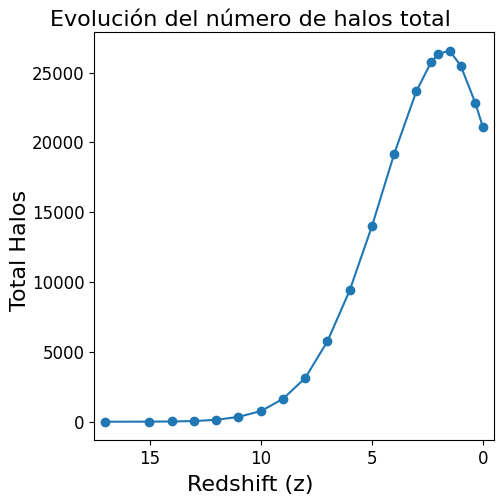
\includegraphics[scale = 0.5]{RunCanonica/TotalHalos_RunCanonica.png}
    \caption[Evolución del número de halos en un Universo $\Omega_\lambda = 0.691 $, $\Omega_0 = 0.309$]{\footnotesize Se muestra el número de halos según el redshift y podemos observar como evoluciona el Universo en una cosmología $\Omega_\lambda = 0.691 $ y $\Omega_0 = 0.309$.}
    \label{fig:Canon_TotalHalos}
\end{figure}

La distribución de la masa para esta cosmología se observa en las figuras \ref{fig:Canon-MassDistSep} y \ref{fig:Canon-MassDist}, donde ajustamos una distribución ex-Gaussian. Los rangos de la masa se encuentran entre las $10^{10.11}$ $M_\odot$ a $10^{14.32}$ $M_\odot$ a lo largo de de la evolución del sistema. Las primeras estructuras, las que tienen $z$ altos, tenían masas menores a $10^{10.65}$ $M_\odot$ en $z=15$ y las estructuras en $z$ pequeños, la mayor parte de los halos tenían masas entre $10^{10.25}$ $M_\odot$ y $10^{11.25}$ $M_\odot$ con estructuras que alcanzan $10^{14.32}$ $M_\odot$ en $z=0$. Mientras, la figura \ref{fig:Canon-MassStats} nos muestra el comportamiento medio durante la evolución donde observamos que la masa media incrementa desde $10^{10.41}$ $M_\odot$ con una desviación de $10^{0.09}$ $M_\odot$ en $z=15$ hasta $10^{10.75}$ $M_\odot$ con una desviación de $10^{0.5}$ $M_\odot$ en $z=0$.

\begin{figure}[H]
    \centering
    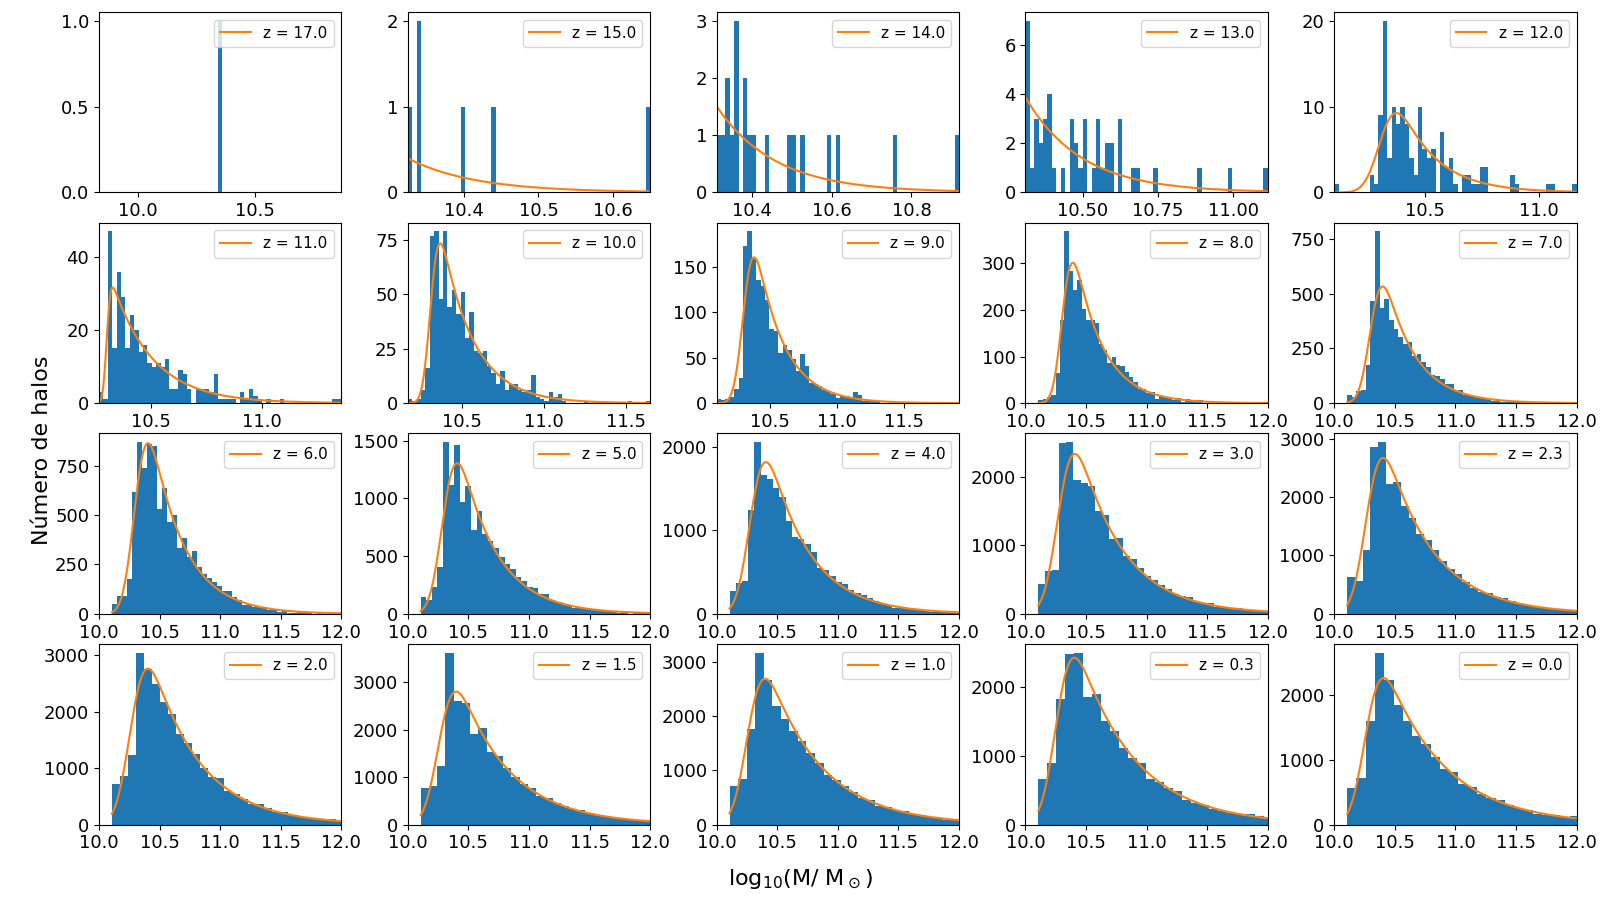
\includegraphics[width = \linewidth]{RunCanonica/Mass_Dist_RunCanonicaSep.png}
    \caption[Distribución de masa]{\footnotesize Mostramos la cantidad de halos en los diferentes rangos de masa y su ajuste conforme evoluciona el Universo en una cosmología $\Omega_\lambda = 0.691 $ y $\Omega_0 = 0.309$. Se muestran las distribuciones en los diferentes redshifts empezando en $z=17$ en la parte superior izquierda y terminado en $z=0$ en la parte inferior derecha. Se observa como aumentan la cantidad de halos cada vez más masivos.}
    \label{fig:Canon-MassDistSep}
\end{figure}

\begin{figure}[H]
    \centering
    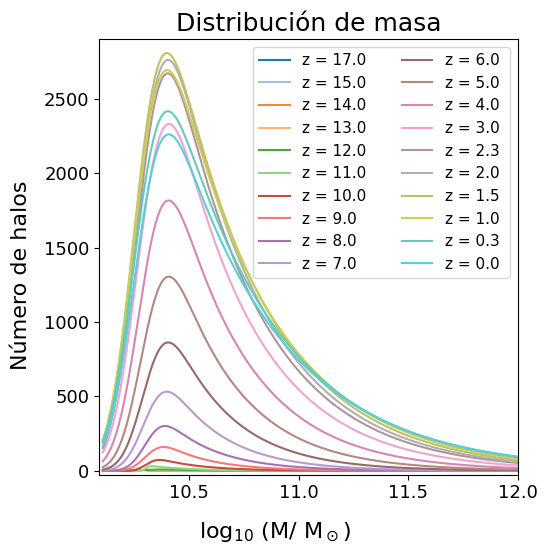
\includegraphics[width = 0.5\linewidth]{RunCanonica/Mass_Dist_RunCanonica.png}
    \caption[Comparación de distribución de masa]{\footnotesize  Mostramos los ajustes de la figura \ref{fig:Canon-MassDistSep} para destacar la evolución de la distribución de masa del Universo $\Omega_\lambda = 0.691 $, $\Omega_0 = 0.309$ desde un $z=17$ hasta un $z=0$.}
    \label{fig:Canon-MassDist}
\end{figure}

\begin{figure}[H]
    \centering
    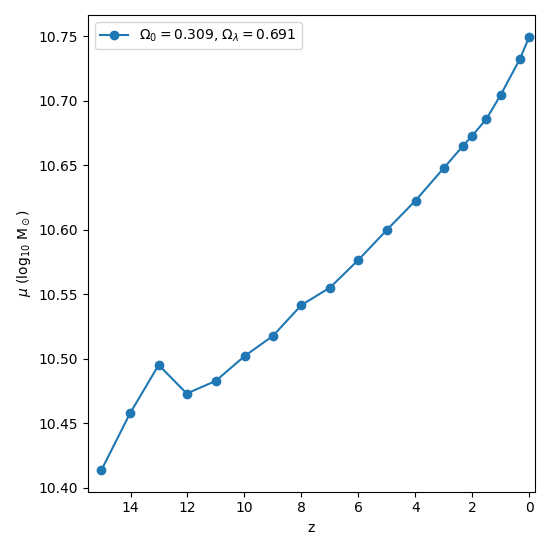
\includegraphics[width = 0.4\linewidth]{RunCanonica/MassMean_RunCanonica.png}
    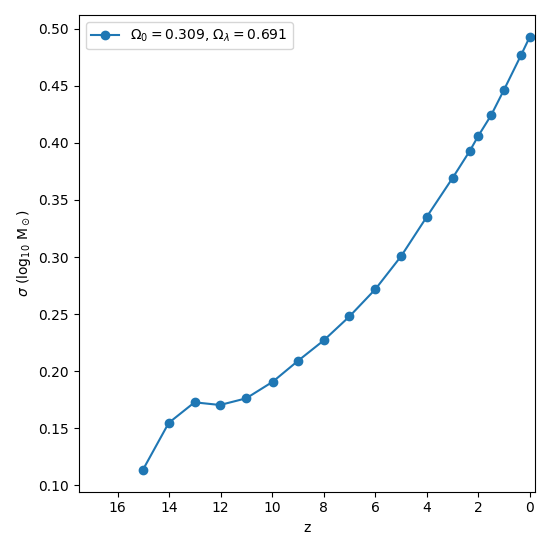
\includegraphics[width = 0.4\linewidth]{RunCanonica/MassStd_RunCanonica.png}
    \caption[Media y desviación estándar de la distribución de masa]{\footnotesize En la izquierda se muestra la masa media de los halos de materia oscura donde observamos como cambian durante la evolución del Universo. En la derecha se muestra la desviación estándar de la masa, la cual nos muestra la variedad de los halos que hay durante la evolución del Universo, desde un $z=17$ hasta un $z=0$.}
    \label{fig:Canon-MassStats}
\end{figure}

En las figuras \ref{fig:Canon-HalfMassRadDistSep} y \ref{fig:Canon-HalfMassRadDist}, donde ajustamos una distribución normal, podemos ver el radio que contiene la mitad de la masa de los halos a lo largo de la evolución del Universo. Vemos que los radios se encuentran entre los $10^{0.33}$ kpc y $10^{2.69}$ kpc a lo largo de la simulación, donde en los redshifts altos, los halos tienen radios entre los $10^{0.33}$ kpc y los $10^{0.51}$ en $z=15$ y las estructuras más recientes tienen la mayor parte de los halos en el rango de $10^{1.28}$ kpc y los $10^{1.66}$ kpc con halos que alcanzan hasta los $10^{2.69}$ kpc en $z=0$. En la figura \ref{fig:Canon-HalfMassRadStats} vemos el crecimiento del radio medio desde $10^{0.44}$ kpc con una desviación de $10^{0.06}$ kpc en $z=15$ hasta un radio de $10^{1.47}$ kpc con una desviación de $10^{0.19}$ kpc en $z=0$.

\begin{figure}[H]
    \centering
    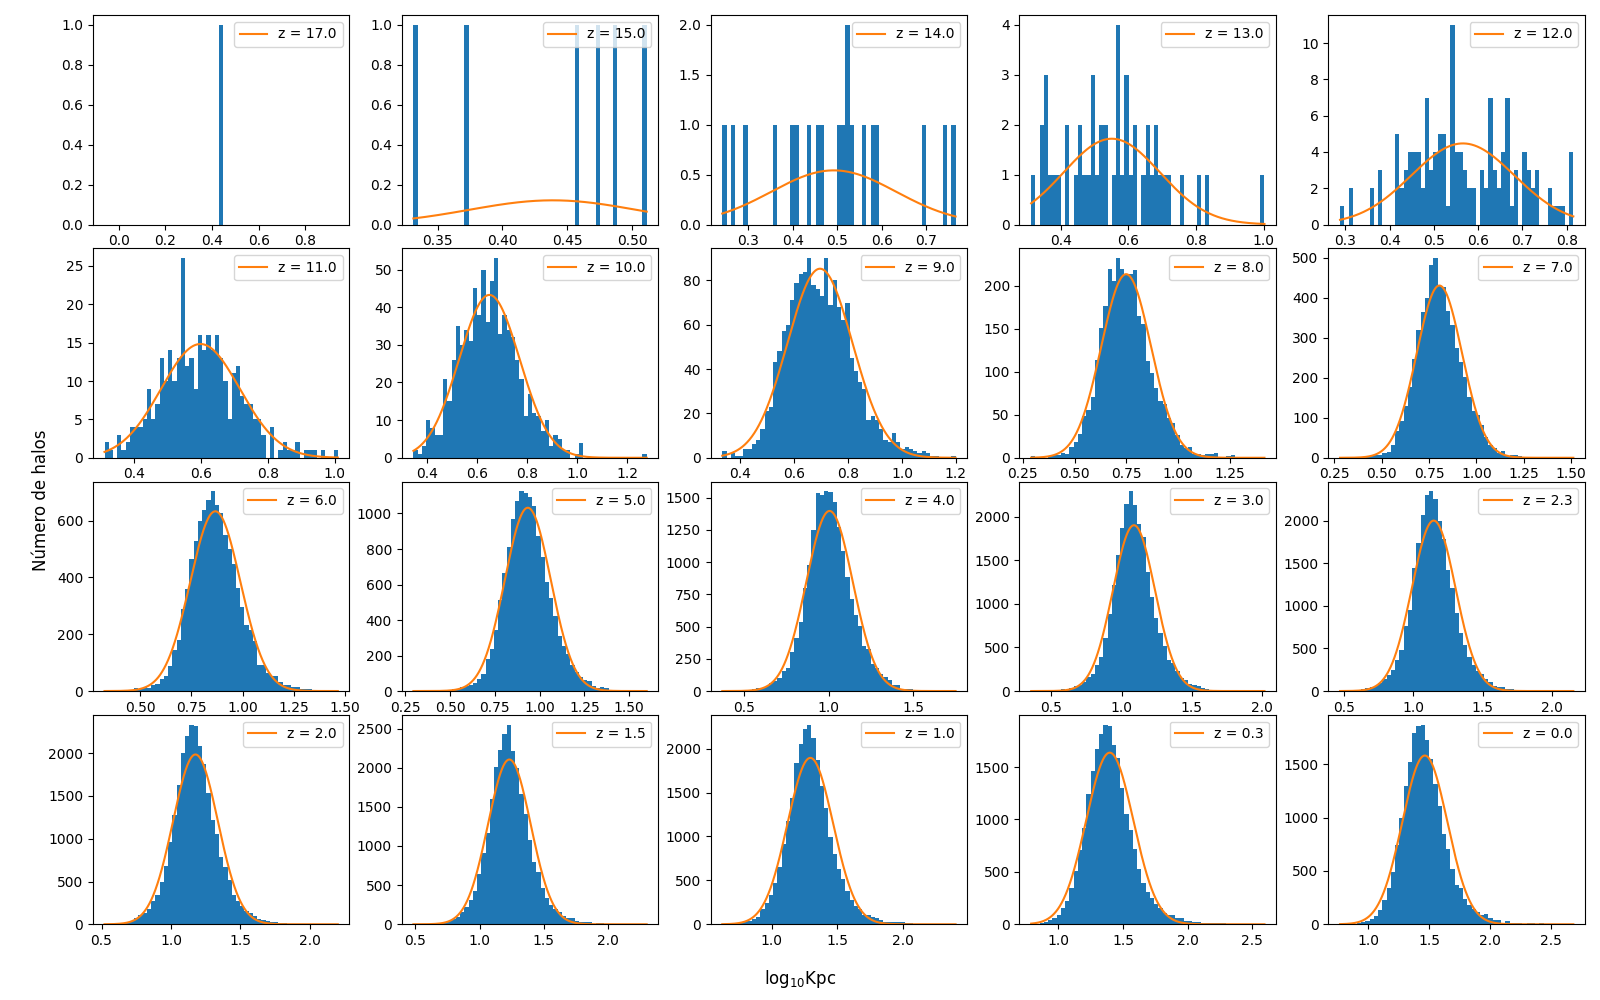
\includegraphics[width = 0.75\linewidth]{RunCanonica/HalfMassRad_Dist_RunCanonicaSep.png}
    \caption[Radio que contiene la mitad de la masa]{\footnotesize Mostramos la cantidad de halos de materia oscura en los diferentes rangos del radio que contiene la mitad de la masa y su ajuste conforme evoluciona en el Universo $\Omega_\lambda = 0.691 $, $\Omega_0 = 0.309$. Se muestran las distribuciones empezando en $z=17$ en la parte superior izquierda y terminado en $z=0$ en la parte inferior derecha.} 
    \label{fig:Canon-HalfMassRadDistSep}
\end{figure}

\begin{figure}[H]
    \centering
    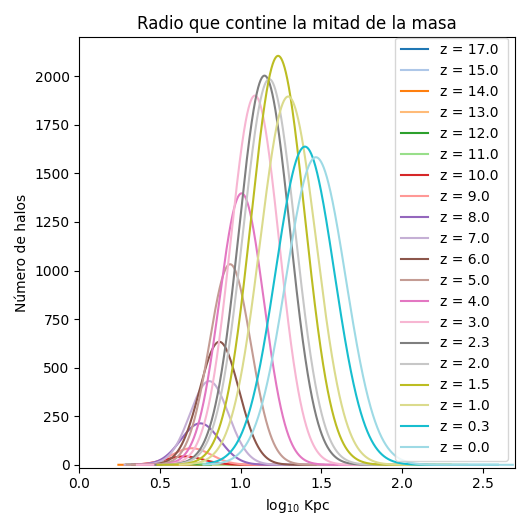
\includegraphics[width = 0.5\linewidth]{RunCanonica/HalfMassRad_Dist_RunCanonica.png}
    \caption[Distribución del radio que contiene la mitad de la masa]{\footnotesize Mostramos los ajustes de la figura \ref{fig:Canon-HalfMassRadDistSep} para destacar la evolución de la distribución del radio que contiene la mitad de la masa del Universo $\Omega_\lambda = 0.691 $, $\Omega_0 = 0.309$ desde un $z=17$ hasta un $z=0$.}
    \label{fig:Canon-HalfMassRadDist}
\end{figure}

\begin{figure}[H]
    \centering
    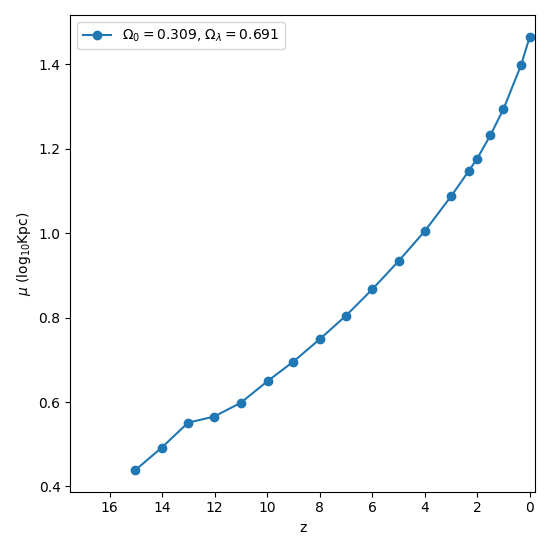
\includegraphics[width = 0.4\linewidth]{RunCanonica/HalfMassRad_Mean_RunCanonica.png}
    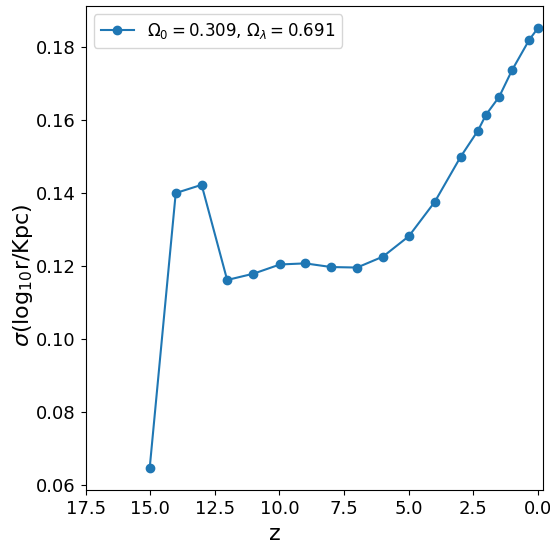
\includegraphics[width = 0.4\linewidth]{RunCanonica/HalfMassRad_Std_RunCanonica.png}
    \caption[Media y desviación estándar del radio de la mitad de la masa]{\footnotesize En la izquierda mostramos la media del radio que contiene la mitad de la masa de los halos de materia oscura donde observamos como cambian durante la evolución del Universo. En la derecha se muestra la desviación estándar del radio que contiene la mitad de la masa que nos muestra la variedad de halos que hay durante la evolución del Universo, desde un $z=17$ hasta un $z=0$.}
    \label{fig:Canon-HalfMassRadStats}
\end{figure}

Otra medida que utilizamos para dar una idea en el tamaño que tienen los halos es usando el radio donde tenemos la mayor velocidad circular. En las figuras \ref{fig:Canon-VMaxRadDistSep} y \ref{fig:Canon-VMaxRadDist}, donde ajustamos una distribución normal, observamos que a lo largo de la evolución de las estructuras, tenemos halos con radios que van desde los $1.44$ kpc hasta los $411.48$ kpc. Vemos que la gran mayoría de los halos tienen tamaños entre $11.91$ kpc y $43.29$ kpc con halos que alcanzan hasta los $411.48$ kpc en $z=0$ y en $z=15$ tenemos halos menores a $3.61$ kpc. En la figura \ref{fig:Canon-VMaxRadStats} vemos que la media va desde los $2.45$ kpc con una desviación de $0.88$ kpc en $z=15$ hasta $27.60$ kpc con una desviación de $15.69$ kpc en $z=0$.

\begin{figure}[H]
    \centering
    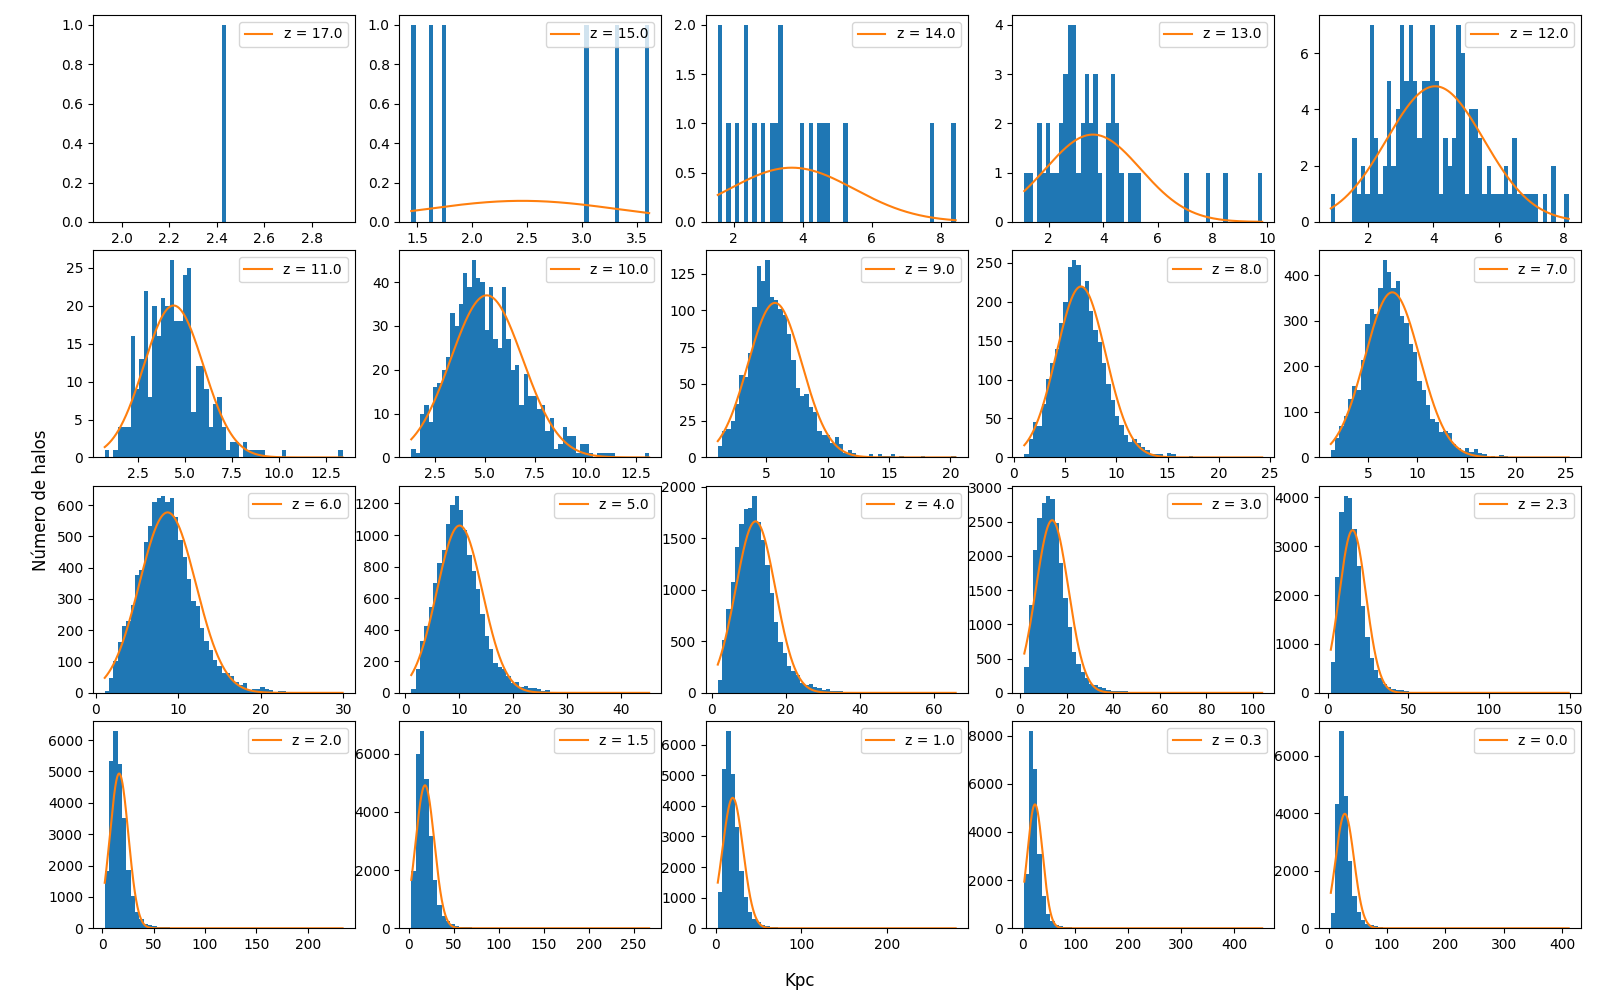
\includegraphics[width = 0.75\linewidth]{RunCanonica/VMaxRad_Dist_RunCanonicaSep.png}
    \caption[Radio donde se alcanza la velocidad máxima circular]{\footnotesize Mostramos la cantidad de halos de materia oscura en los diferentes rangos del radio donde alcanza su velocidad máxima circular y su ajuste conforme evoluciona en el Universo $\Omega_\lambda = 0.691 $, $\Omega_0 = 0.309$. Se muestran las distribuciones empezando en $z=17$ en la parte superior izquierda y terminado en $z=0$ en la parte inferior derecha.}
    \label{fig:Canon-VMaxRadDistSep}
\end{figure}

\begin{figure}[H]
    \centering
    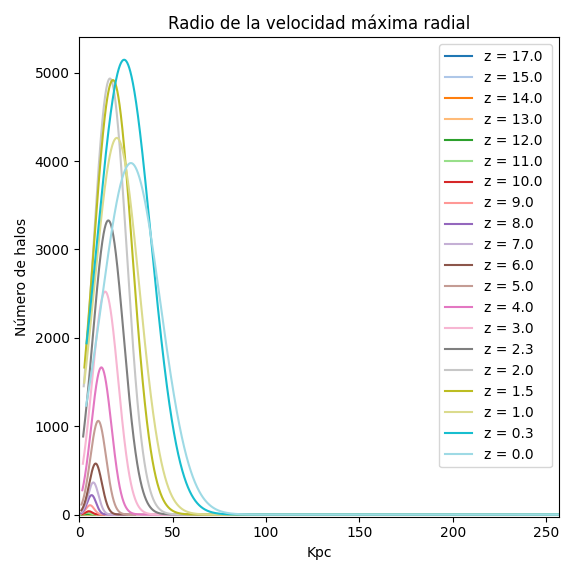
\includegraphics[width = 0.5\linewidth]{RunCanonica/VMaxRad_Dist_RunCanonica.png}
    \caption[Distribución del radio donde se alcanza la velocidad máxima circular]{\footnotesize Mostramos los ajustes de la figura \ref{fig:Canon-VMaxRadDistSep} para destacar la evolución de la distribución del radio donde alcanza su velocidad máxima circular del Universo $\Omega_\lambda = 0.691 $, $\Omega_0 = 0.309$ desde un $z=17$ hasta un $z=0$.}
    \label{fig:Canon-VMaxRadDist}
\end{figure}

\begin{figure}[H]
    \centering
    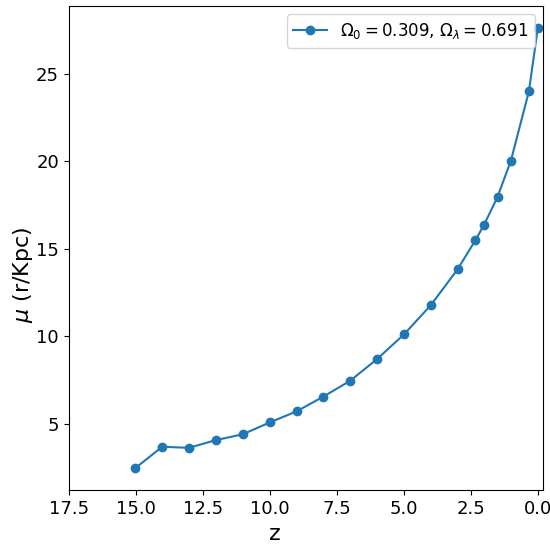
\includegraphics[width = 0.4\linewidth]{RunCanonica/VMaxRad_Mean_RunCanonica.png}
    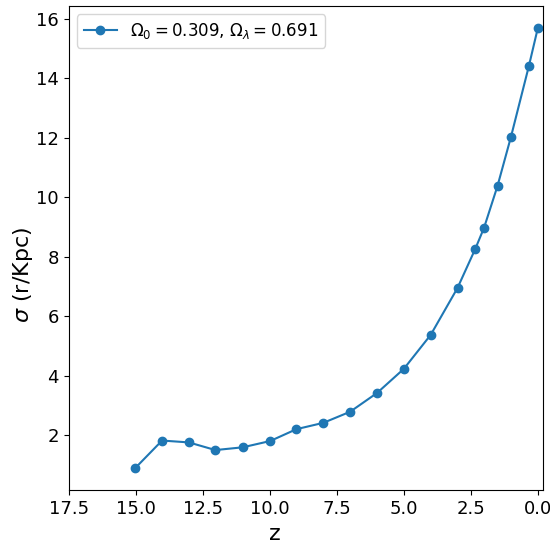
\includegraphics[width = 0.4\linewidth]{RunCanonica/VMaxRad_Std_RunCanonica.png}
    \caption[Media y desviación estándar del Radio donde se alcanza la velocidad máxima circular]{\footnotesize En la izquierda mostramos la media del radio donde alcanza su velocidad máxima circular en los halos de materia oscura donde observamos como cambian durante la evolución del Universo. En la derecha se muestra la desviación estándar del radio donde alcanza su velocidad máxima circular que nos muestra la variedad de halos que hay durante la evolución del Universo, desde un $z=17$ hasta un $z=0$.}
    \label{fig:Canon-VMaxRadStats}
\end{figure}

Continuando con las velocidades, empezamos con la velocidad circular máxima, donde ajustamos una distribución ex-Gaussian. Podemos apreciar que las velocidades circulares van de los rangos de los $22.82$ kms$^{-1}$ hasta los $992.53$ kms$^{-1}$ donde vemos la gran mayoría de los halos entre los $123.37$ kms$^{-1}$ y $176.89$ kms$^{-1}$ en $z=15$ y entre los $40.87$ kms$^{-1}$ y $108.67$ kms$^{-1}$ en $z=0$, como se muestra en las figuras \ref{fig:Canon-VelMaxDistSep} y \ref{fig:Canon-VelMaxDist}. Lo que podemos ver en la figura \ref{fig:Canon-VelMaxStats} es que la velocidad media disminuye rápidamente desde $150.13$ kms$^{-1}$ con una desviación de $26.76$ kms$^{-1}$ en $z=15$ hasta que alcanza $74.77$ kms$^{-1}$ con una desviación de $33.90$ kms$^{-1}$ en $z=0$.

\begin{figure}[H]
    \centering
    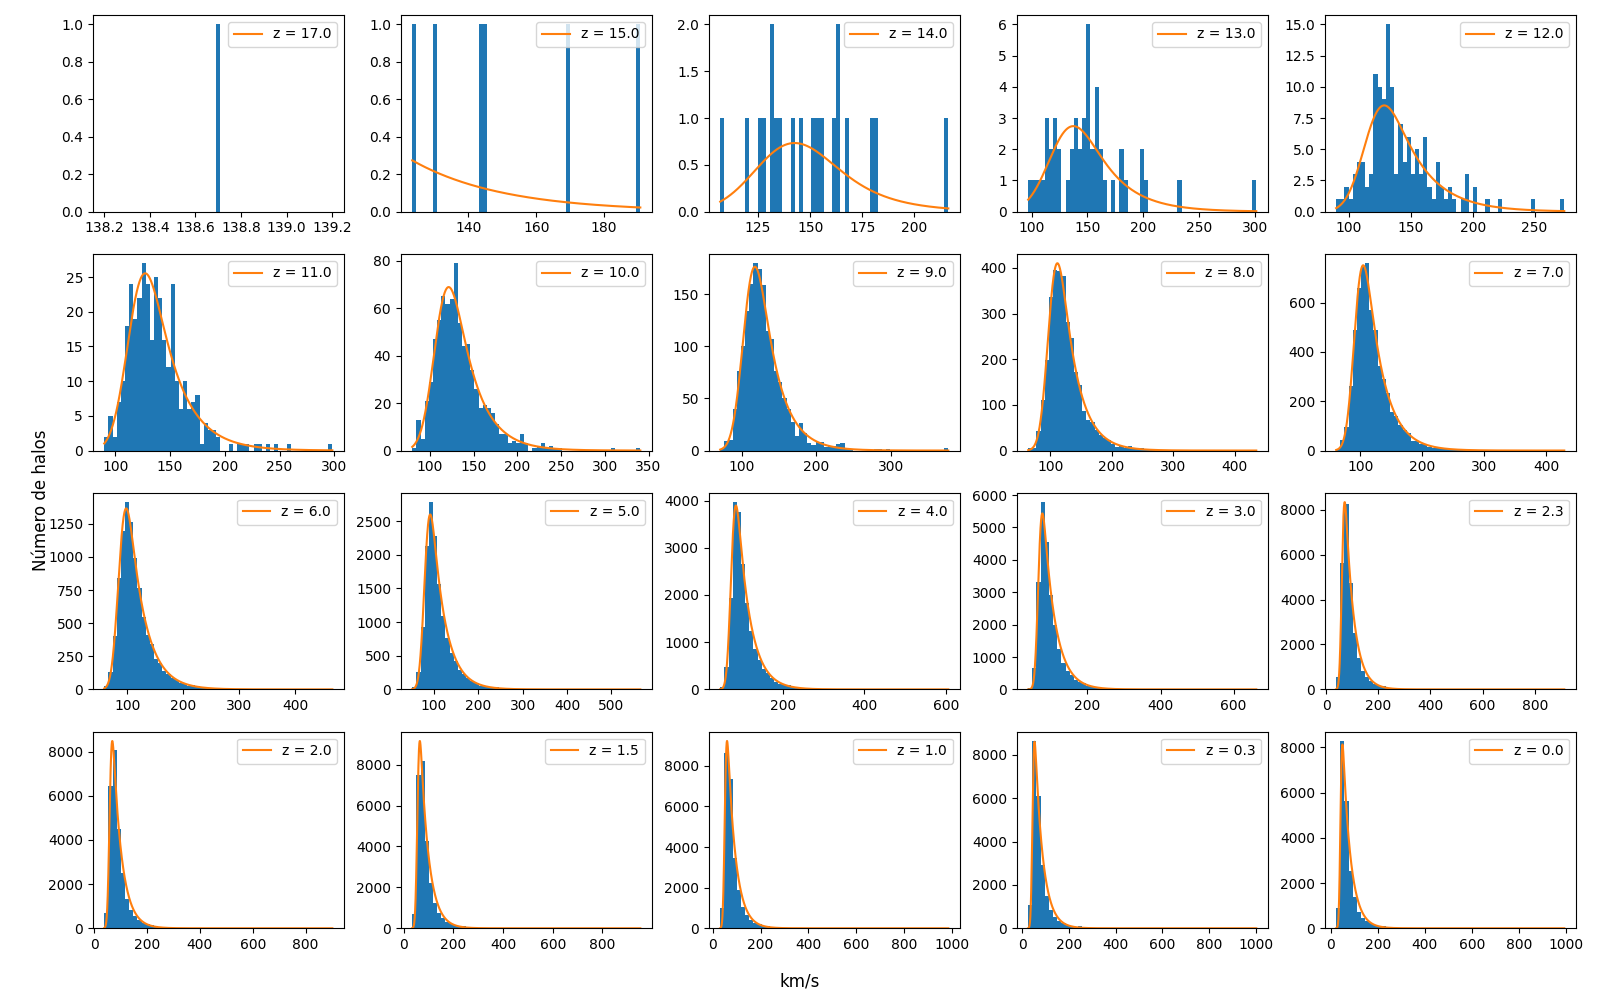
\includegraphics[width = 0.75\linewidth]{RunCanonica/VelMax_Dist_RunCanonicaSep.png}
    \caption[Velocidad circular máxima]{\footnotesize Mostramos la cantidad de halos de materia oscura en los diferentes rangos de la velocidad circular máxima y su ajuste conforme evoluciona en el Universo $\Omega_\lambda = 0.691 $, $\Omega_0 = 0.309$. Se muestran las distribuciones empezando en $z=17$ en la parte superior izquierda y terminado en $z=0$ en la parte inferior derecha.}
    \label{fig:Canon-VelMaxDistSep}
\end{figure}

\begin{figure}[H]
    \centering
    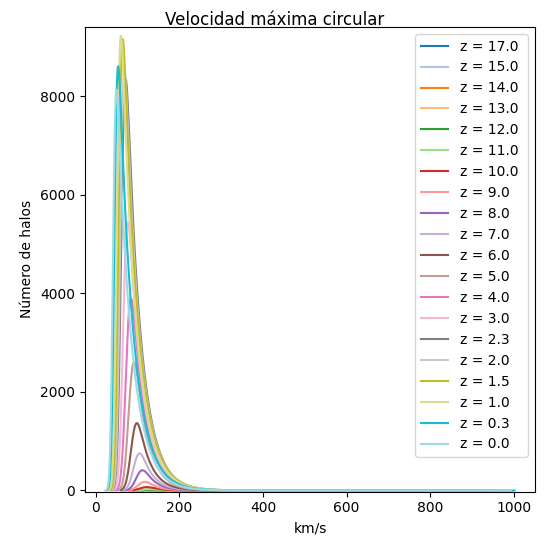
\includegraphics[width = 0.5\linewidth]{RunCanonica/VelMax_Dist_RunCanonica.png}
    \caption[Distribución de la velocidad circular máxima]{\footnotesize Mostramos los ajustes de la figura \ref{fig:Canon-VelMaxDistSep} para destacar la evolución de la distribución de la velocidad circular máxima del Universo $\Omega_\lambda = 0.691 $, $\Omega_0 = 0.309$ desde un $z=17$ hasta un $z=0$.}
    \label{fig:Canon-VelMaxDist}
\end{figure}

\begin{figure}[H]
    \centering
    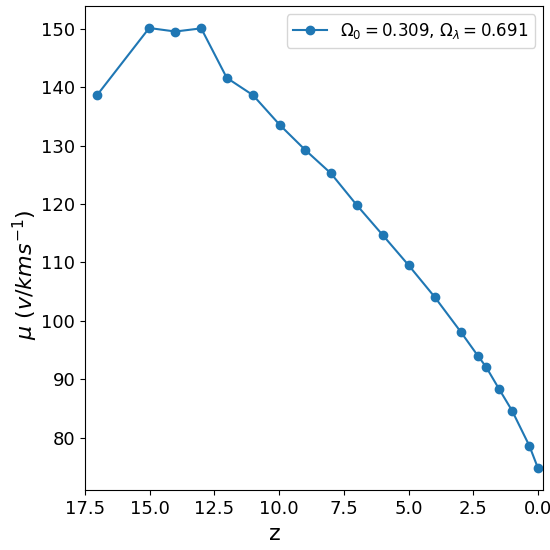
\includegraphics[width = 0.4\linewidth]{RunCanonica/VelMax_Mean_RunCanonica.png}
    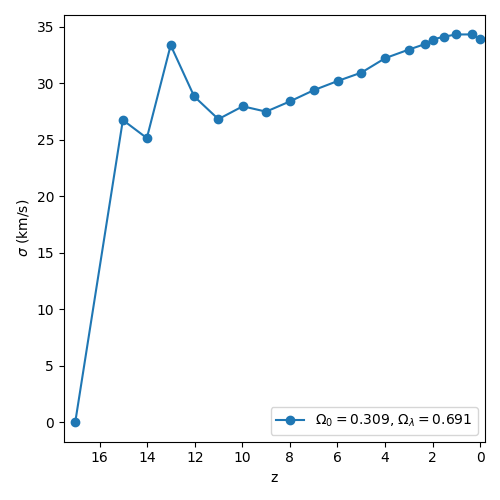
\includegraphics[width = 0.4\linewidth]{RunCanonica/VelMax_Std_RunCanonica.png}
    \caption[Media y desviación estándar de la velocidad circular máxima]{\footnotesize En la izquierda mostramos la media de la velocidad circular máxima en los halos de materia oscura donde observamos como cambian durante la evolución del Universo. En la derecha se muestra la desviación estándar de la velocidad circular máxima que nos muestra la variedad de halos que hay durante la evolución del Universo, desde un $z=17$ hasta un $z=0$.}
    \label{fig:Canon-VelMaxStats}
\end{figure}

Ahora hablemos de la dispersión de las velocidades de los halos de materia oscura. La dispersión de velocidades de estos halos esta entre $12.78$ kms$^{-1}$ a los $572.55$ kms$^{-1}$ a lo largo de la evolución de los halos. Vemos en las figuras \ref{fig:Canon-VelDispDistSep} y \ref{fig:Canon-VelDispDist}, donde ajustamos una distribución ex-Gaussian}, que en $z=15$ la mayor parte de los halos se encuentran en el rango de los $72.16$ kms$^{-1}$ a los $98.34$ kms$^{-1}$ con picos en los $107.89$ kms$^{-1}$, mientras que en $z=0$ vemos la mayor parte de los halos con velocidades que van entre $18.39$ kms$^{-1}$ y $55.77$ kms$^{-1}$ con picos en $572.55$ kms$^{-1}$. En la figura \ref{fig:Canon-VelDispStats} observamos que la dispersión de velocidades media disminuye desde los $85.25$ kms$^{-1}$ con una desviación de $13.09$ kms$^{-1}$ en $z=15$ a $37.08$ kms$^{-1}$ con una desviación de $18.69$ kms$^{-1}$ en $z=0$.

\begin{figure}[H]
    \centering
    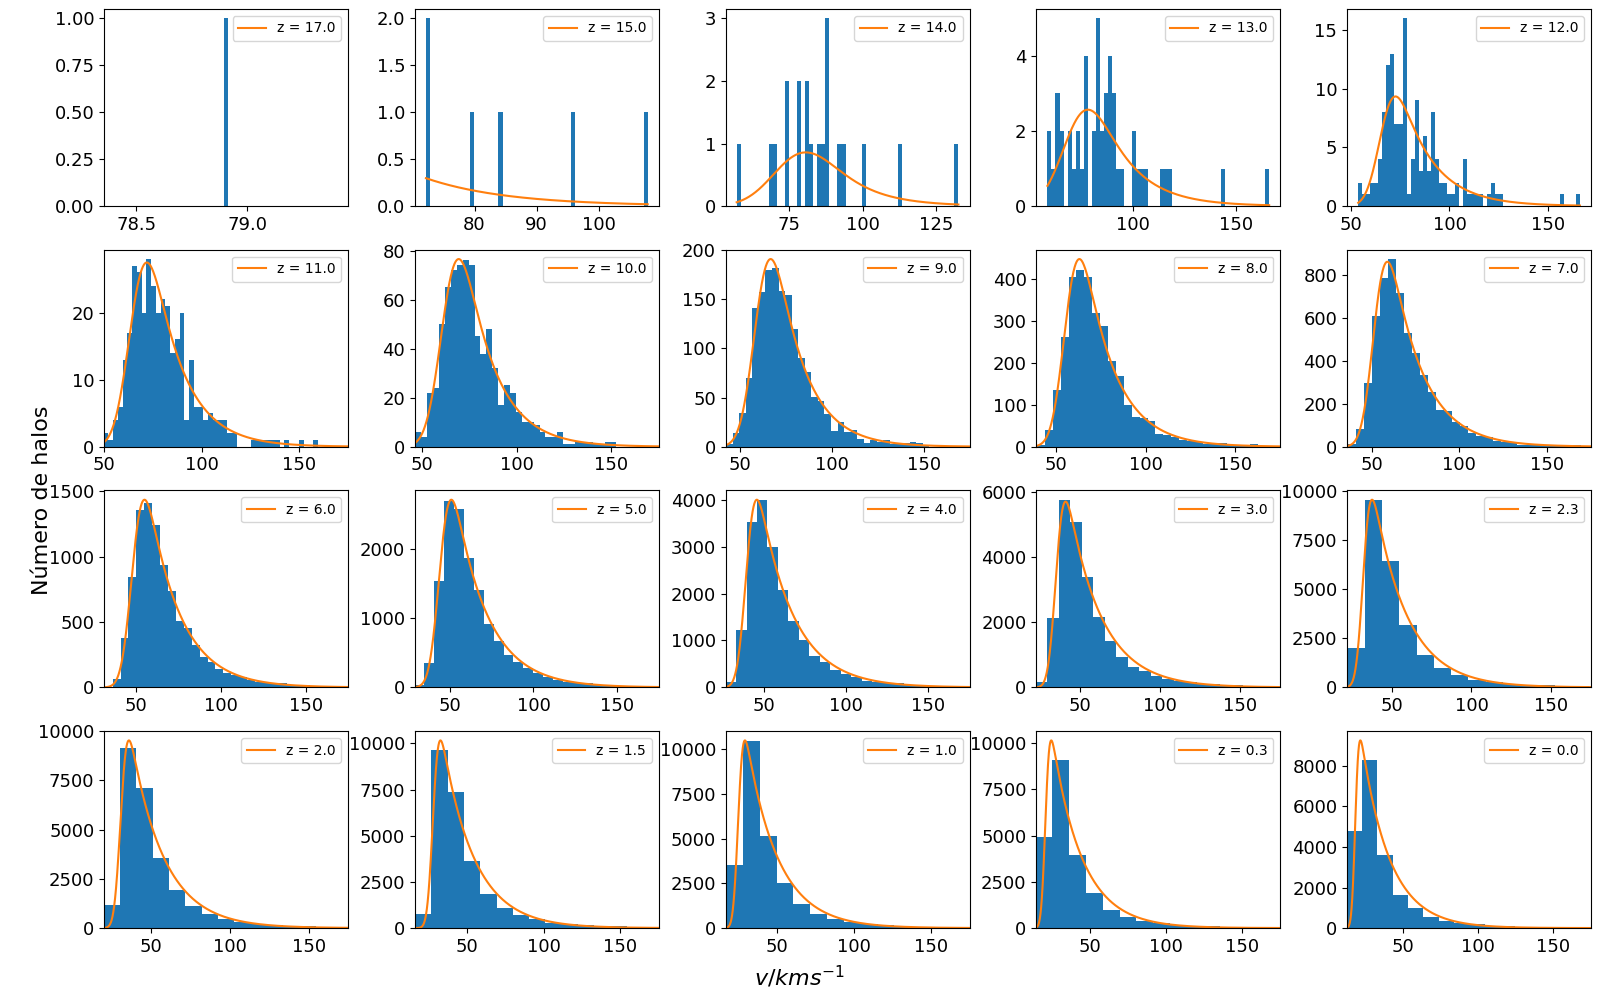
\includegraphics[width = 0.75\linewidth]{RunCanonica/VelDisp_Dist_RunCanonicaSep.png}
    \caption[Dispersión de velocidades]{\footnotesize Mostramos la cantidad de halos en los diferentes rangos de la dispersión de velocidades y su ajuste conforme evoluciona el Universo $\Omega_\lambda = 0.691 $, $\Omega_0 = 0.309$. Se muestran las distribuciones empezando en $z=17$ en la parte superior izquierda y terminando en $z=0$ en la parte inferior derecha.}
    \label{fig:Canon-VelDispDistSep}
\end{figure}

\begin{figure}[H]
    \centering
    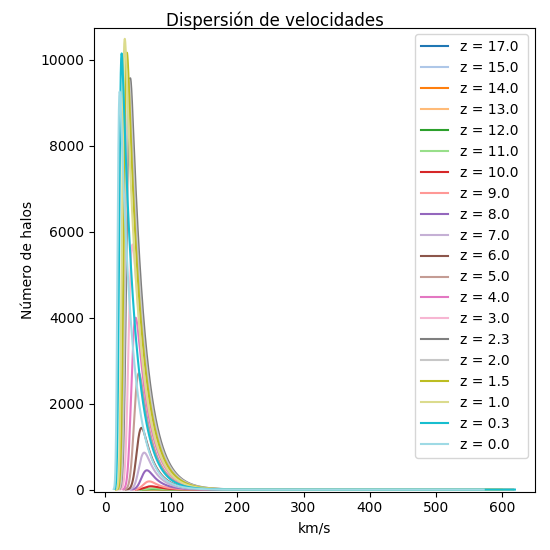
\includegraphics[width = 0.5\linewidth]{RunCanonica/VelDisp_Dist_RunCanonica.png}
    \caption[Distribución de la dispersión de velocidades]{\footnotesize Mostramos los ajustes de la figura \ref{fig:Canon-VelDispDistSep} para destacar la evolución de la distribución de la dispersión de velocidades del Universo $\Omega_\lambda = 0.691 $, $\Omega_0 = 0.309$ desde un $z=17$ hasta un $z=0$.}
    \label{fig:Canon-VelDispDist}
\end{figure}

\begin{figure}[H]
    \centering
    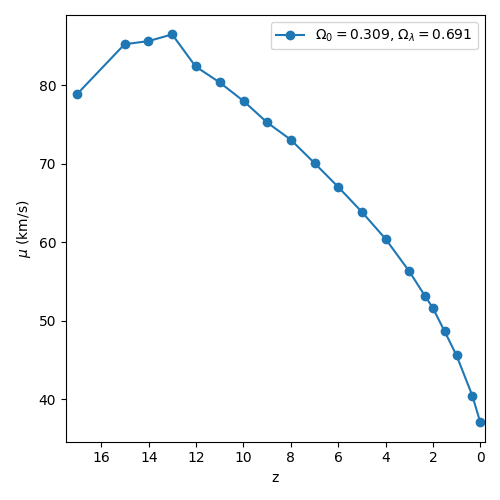
\includegraphics[width = 0.4\linewidth]{RunCanonica/VelDisp_Mean_RunCanonica.png}
    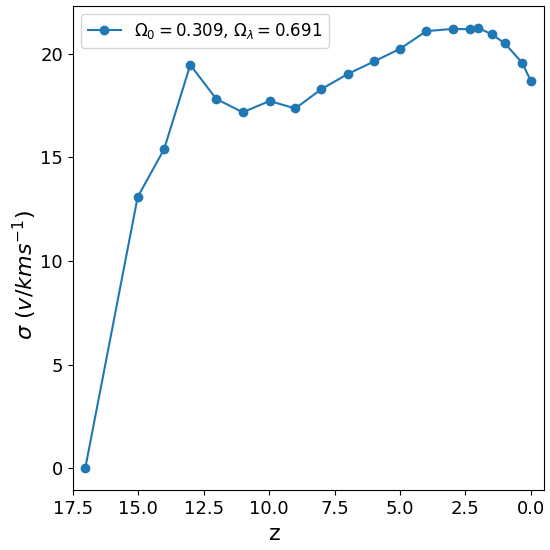
\includegraphics[width = 0.4\linewidth]{RunCanonica/VelDisp_Std_RunCanonica.png}
    \caption[Media y desviación estándar de la dispersión de velocidades]{\footnotesize En la izquierda mostramos la media de la dispersión de velocidades en los halos de materia oscura donde observamos como cambian durante la evolución del Universo. En la derecha se muestra la desviación estándar de la dispersión de velocidades que nos muestra la variedad de halos que hay durante la evolución del Universo, desde un $z=17$ hasta un $z=0$.}
    \label{fig:Canon-VelDispStats}
\end{figure}

Finalmente, la figura \ref{fig:CanonRunDensityMap} muestra a lo que conocemos como la \emph{Cosmic Web} vista desde un plano. Se ve el mapa de densidad de la simulación del Universo en diferentes redshifts. En los redshift altos (viendo más al pasado) se observan nubes difusas donde no hay una estructura, mientras que los redshift bajos (más al presente) se observan estructuras mejor definidas y con el tiempo vemos que hay un aumento en la cantidad de estructura que se observa.

\begin{figure}[H]
    \centering

    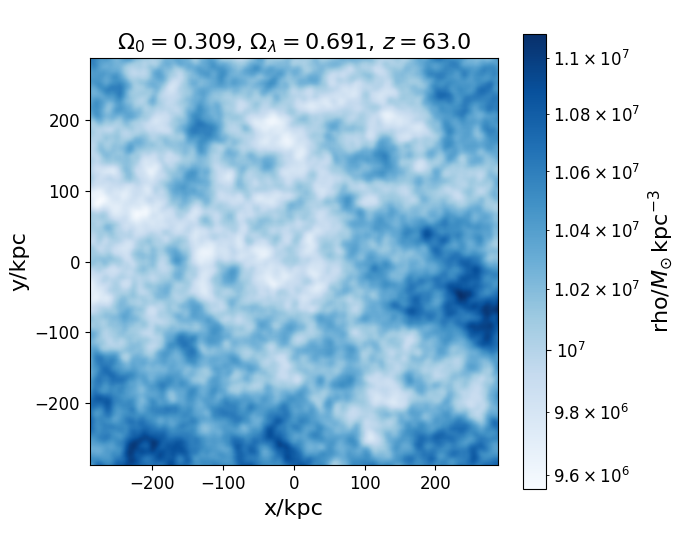
\includegraphics[width = 0.33\linewidth]{RunCanonica/RunCanonicaZ63.png}   %snap 000 z=63
    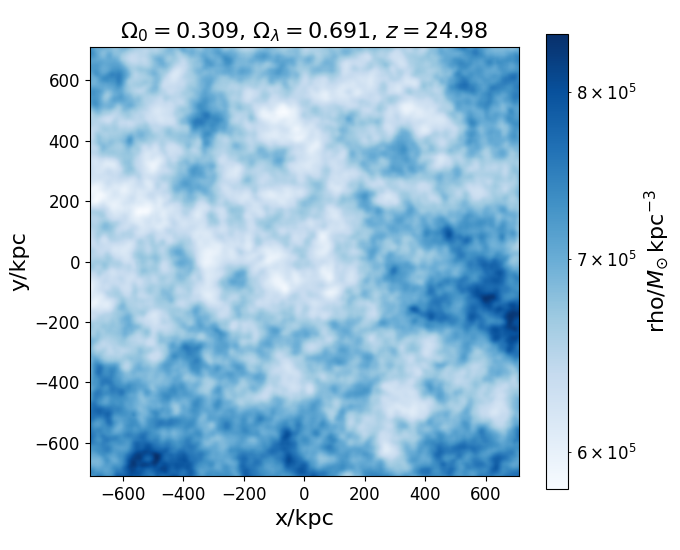
\includegraphics[width = 0.33\linewidth]{RunCanonica/RunCanonicaZ25.png}   %snap 005 z=25
    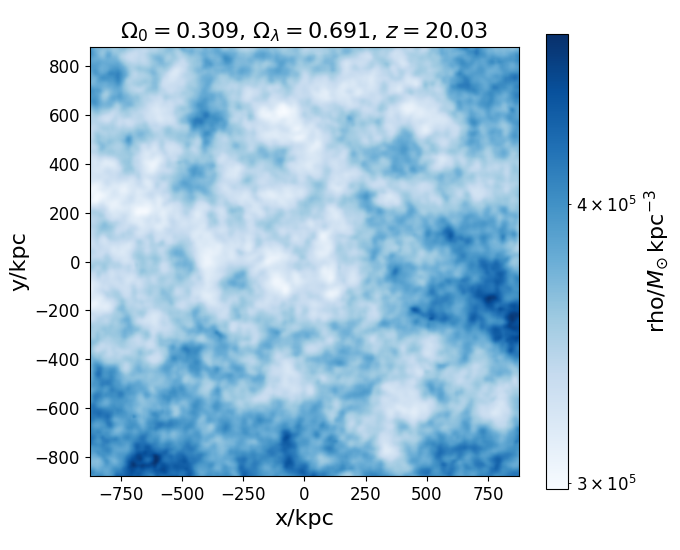
\includegraphics[width = 0.32\linewidth]{RunCanonica/RunCanonicaZ20.png}   %snap 010 z=20
    \\
    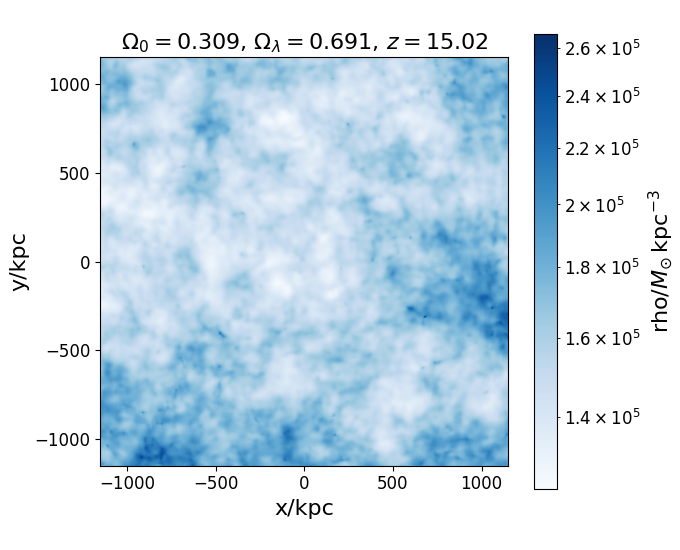
\includegraphics[width = 0.33\linewidth]{RunCanonica/RunCanonicaZ15.png}   %snap 015 z=15
    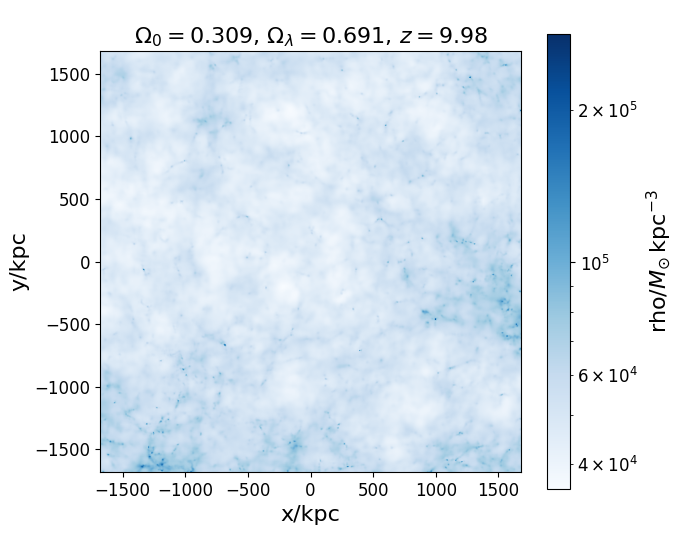
\includegraphics[width = 0.33\linewidth]{RunCanonica/RunCanonicaZ10.png}   %snap 020 z=10
    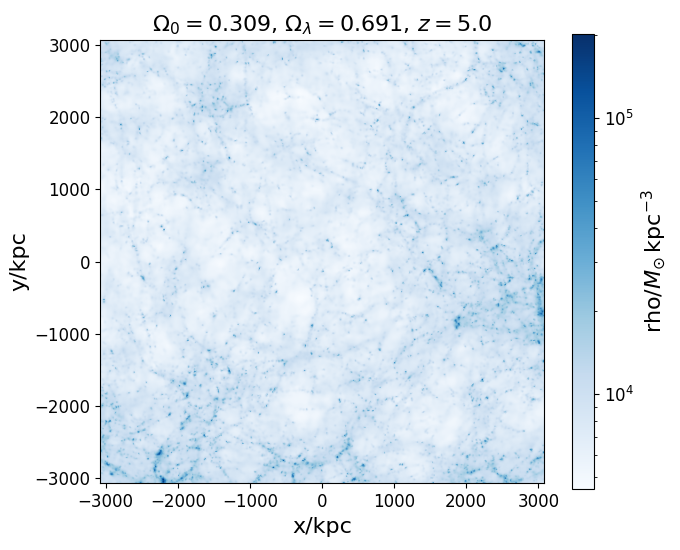
\includegraphics[width = 0.32\linewidth]{RunCanonica/RunCanonicaZ5.png}    %snap 025 z=5
    \\
    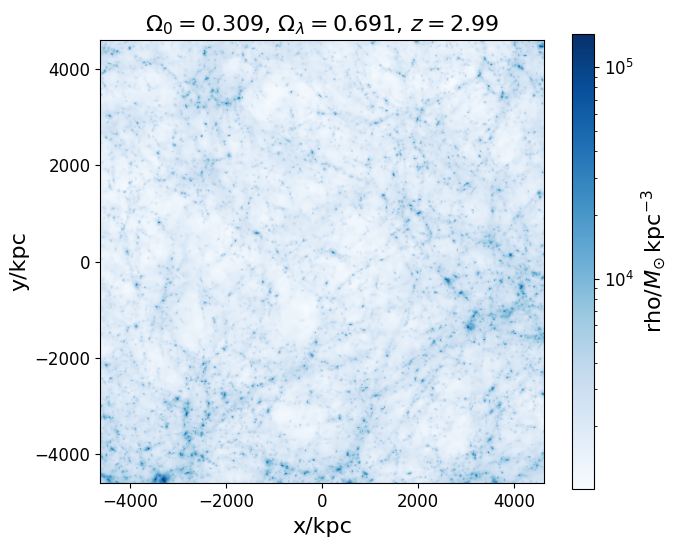
\includegraphics[width = 0.33\linewidth]{RunCanonica/RunCanonicaZ3.png}    %snap 027 z=3
    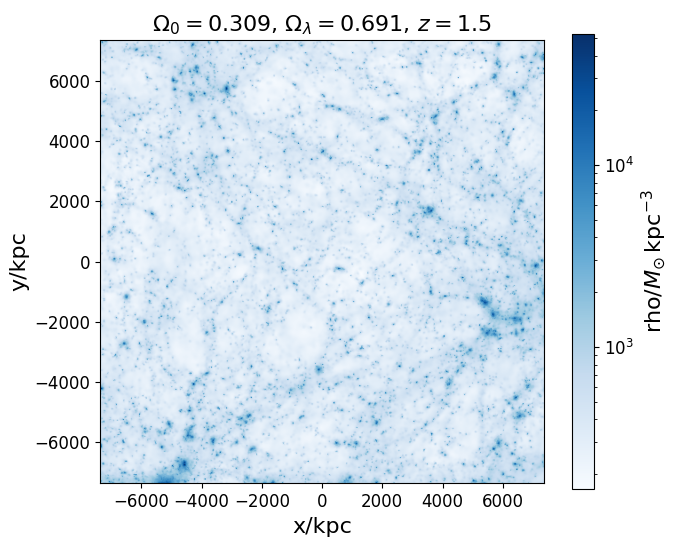
\includegraphics[width = 0.33\linewidth]{RunCanonica/RunCanonicaZ1_5.png}  %snap 030 z=1.5
    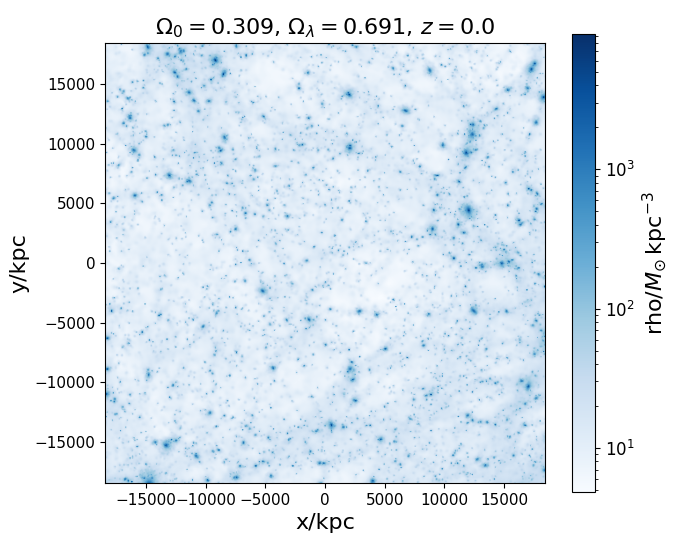
\includegraphics[width = 0.32\linewidth]{RunCanonica/RunCanonicaZ0.png}    %snap 033 z=0
    \caption[Mapa de densidad de un Universo en en diferentes redshift]{ \footnotesize Mapa de densidad de la simulación en diferentes redshifts de una cosmología $\Omega_\lambda = 0.691 $, $\Omega_0 = 0.309$. }
    \label{fig:CanonRunDensityMap}
\end{figure}

%====================================================================================================================
%=====================================  RUN INVERTIDA  ==============================================================
%====================================================================================================================
\subsection{Universo con cosmología  \texorpdfstring{$\Omega_\lambda = 0.309$, $\Omega_0 = 0.691$ }{Omega lambda = 0.309, Omega 0 = 0.691} }
Hemos estudiado un Universo con las densidades más aceptadas, pero como cambia si las densidades cambian, para este caso que sucede si invertimos las densidades pero dejamos el Universo plano. Primeramente podemos apreciar en la figura \ref{fig:Invertida-TotalHalos} que los halos se empiezan a formar en redshift $z=14$ pero tiene un comportamiento similar a la cosmología anterior, teniendo el pico en la cantidad de halos alrededor del redshift $z=2$. 

\begin{figure}[H]
    \centering
    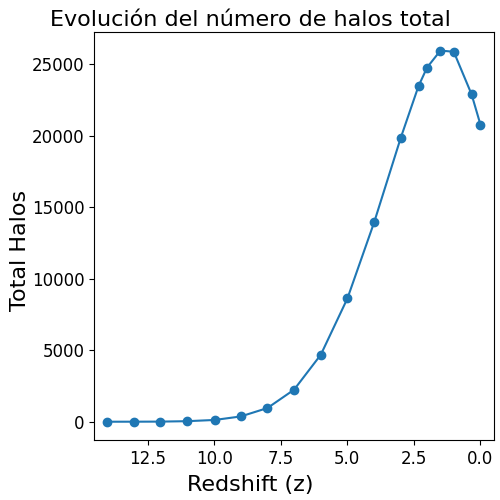
\includegraphics[scale = 0.5]{RunInvertida/TotalHalos_RunInvertida.png}
    \caption[Evolución del número de halos en un Universo $\Omega_\lambda = 0.309 $, $\Omega_0 = 0.691$]{\footnotesize Se muestra el número de halos y como cambia la cantidad conforme evoluciona el Universo en una cosmología $\Omega_\lambda = 0.309 $ y $\Omega_0 = 0.691$.}    
    \label{fig:Invertida-TotalHalos}
\end{figure}

La distribución de masa de este Universo en los diferentes redshifts, se observa en la figura \ref{fig:Invertida-MassDist}. En este Universo los halos tienen una masa de entre $10^{10.46}$ $M_\odot$ y $10^{14.65}$ $M_\odot$ a lo largo de la simulación. En $z=13$ se forman estructuras con masa entre $10^{10.67}$ $M_\odot$ y $10^{10.90}$ $M_\odot$ , mientras que $z=0$ la mayor parte de los halos tienen entre $10^{10.60}$ $M_\odot$ y $10^{11.58}$ $M_\odot$. Además en la figura \ref{fig:Invertida-MassStats} vemos que la media muestra un incremento en la masa de los halos, el que va de $10^{10.79}$ $M\odot$ con una desviación $10^{0.09}$ $M\odot$ en $z=13$ hasta $10^{11.09}$ $M_\odot$ con una desviación de $10^{0.49}$ $M_\odot$ en $z=0$. 

\begin{figure}[H]
    \centering
    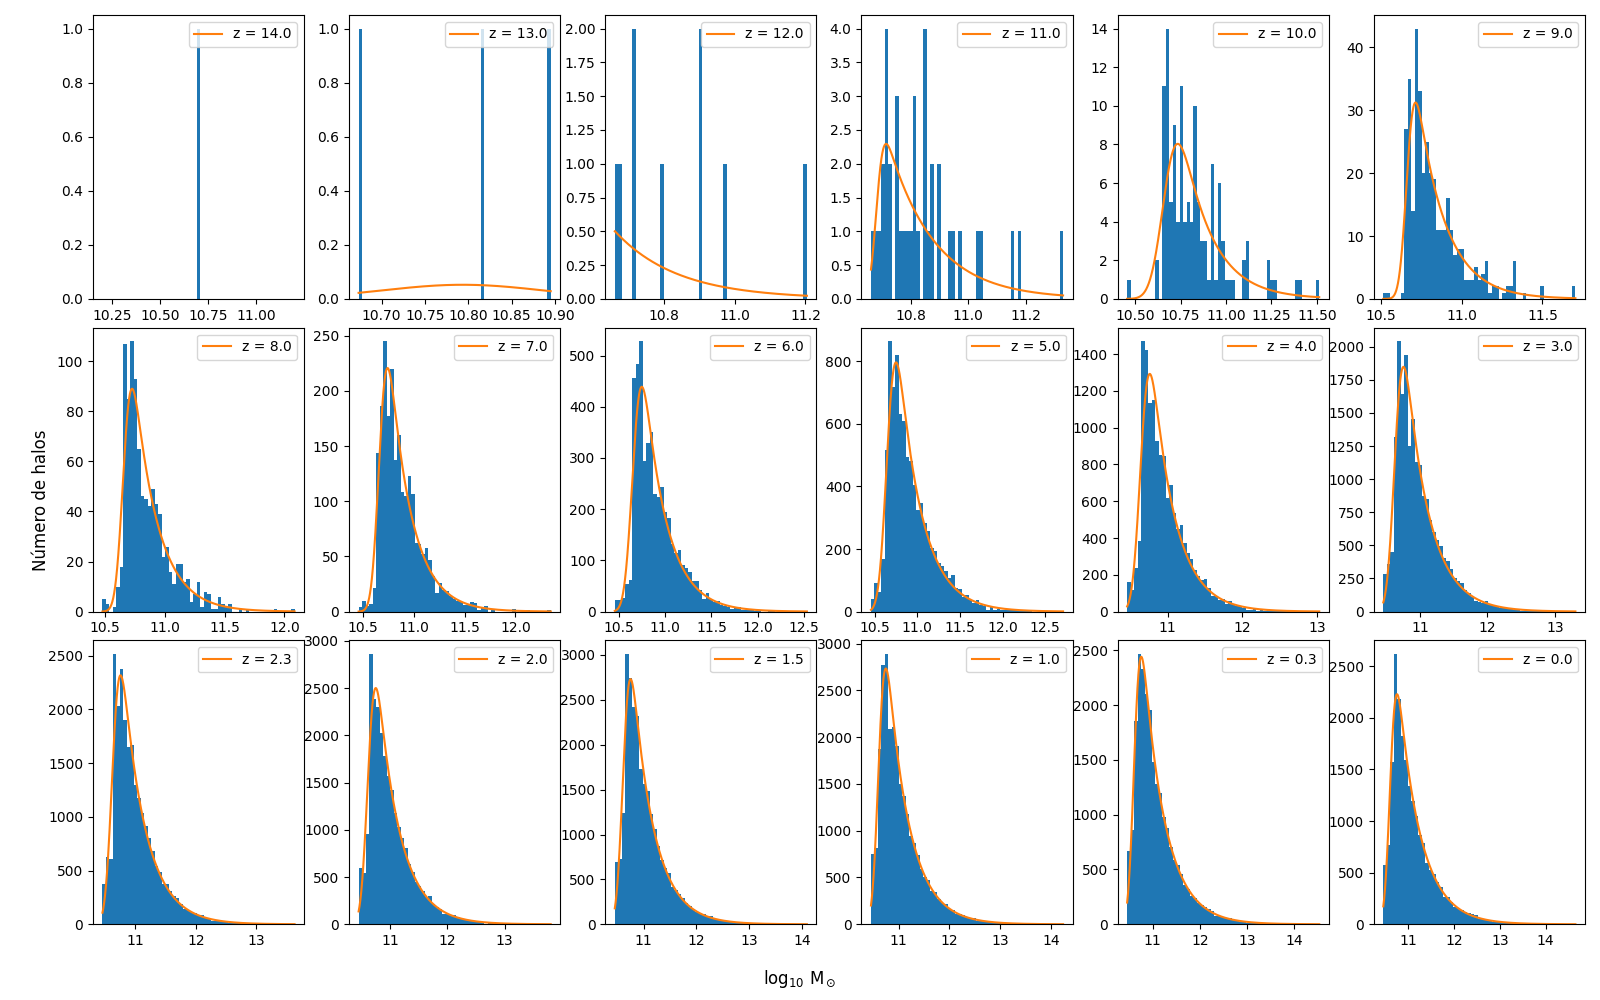
\includegraphics[width = 0.8\linewidth]{RunInvertida/Mass_Dist_RunInvertidaSep.png}
    \caption[Distribución de masa]{\footnotesize Mostramos la cantidad de halos en los diferentes rangos de masa y su ajuste conforme evoluciona el Universo en una cosmología $\Omega_\lambda = 0.309 $ y $\Omega_0 = 0.691$. Se muestran las distribuciones en los diferentes redshifts empezando en $z=14$ en la parte superior izquierda y terminado en $z=0$ en la parte inferior derecha. Se observa como aumentan la cantidad de halos cada vez más masivos.}
    \label{fig:Invertida-MassDistSep}
\end{figure}

\begin{figure}[H]
    \centering
    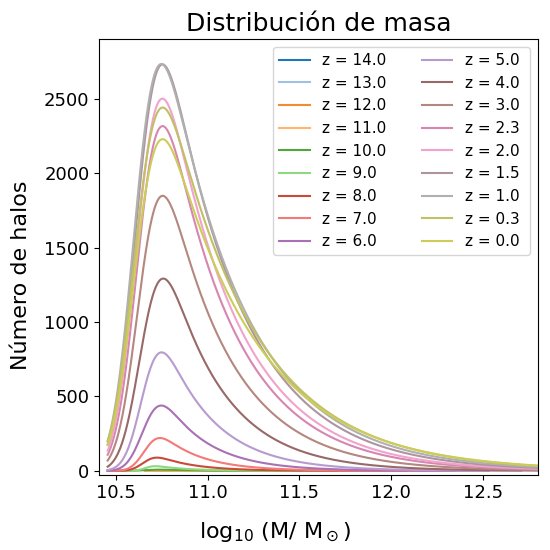
\includegraphics[width = 0.5\linewidth]{RunInvertida/Mass_Dist_RunInvertida.png}
    \caption[Comparación de distribución de masa]{\footnotesize Mostramos los ajustes de la figura \ref{fig:Invertida-MassDistSep} para destacar la evolución de la distribución de masa del Universo $\Omega_\lambda = 0.309 $, $\Omega_0 = 0.691$ desde un $z=14$ hasta un $z=0$.}
    \label{fig:Invertida-MassDist}
\end{figure}

\begin{figure}[H]
    \centering
    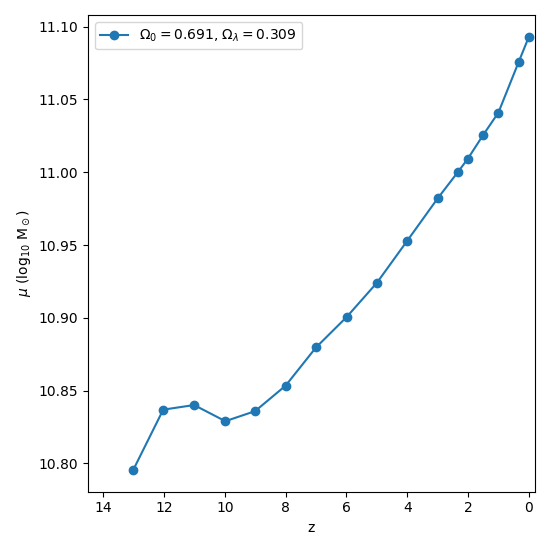
\includegraphics[width = 0.4\linewidth]{RunInvertida/MassMean_RunInvertida.png}
    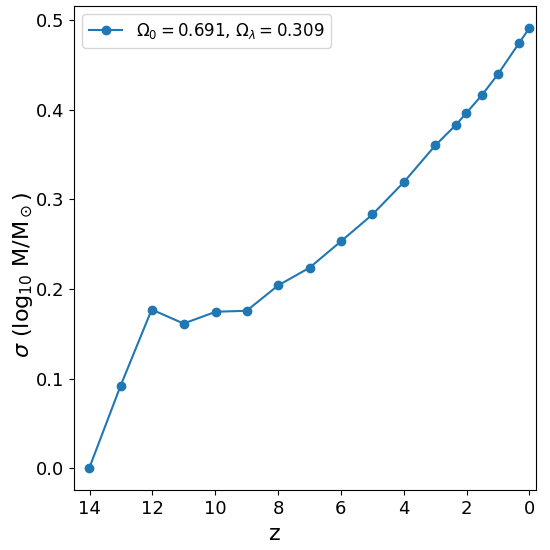
\includegraphics[width = 0.4\linewidth]{RunInvertida/MassStd_RunInvertida.png}
    \caption[Media y desviación estándar de la distribución de masa]{\footnotesize En la izquierda se muestra la masa media de los halos de materia oscura donde observamos como cambian durante la evolución del Universo. En la derecha se muestra la desviación estándar de la masa, la cual nos muestra la variedad de los halos que hay durante la evolución del Universo, desde un $z=14$ hasta un $z=0$.}
    \label{fig:Invertida-MassStats}
\end{figure}

En cuanto al radio que contiene la mitad de la masa, en la figura \ref{fig:Invertida-HalfMassRadDistSep} y \ref{fig:Invertida-HalfMassRadDist} vemos que tenemos halos que tienen radios desde $10^{0.42}$ kpc hasta $10^{2.74}$ kpc a lo largo de la evolución del Universo, donde en $z=13$ tenemos radios entre $10^{0.42}$ kpc y $10^{0.60}$ kpc y en $z=0$ tenemos la mayor parte de los halos entre $10^{1.31}$ kpc y $10^{1.69}$ kpc. En la figura \ref{fig:Invertida-HalfMassRadStats} tenemos que el radio crece con el tiempo, donde el crecimiento va desde $10^{0.53}$ kpc con una desviación de $10^{0.08}$ kpc en $z=13$ hasta $10^{1.5}$ kpc con una desviación de $10^{0.19}$ kpc en $z=0$.

\begin{figure}[H]
    \centering
    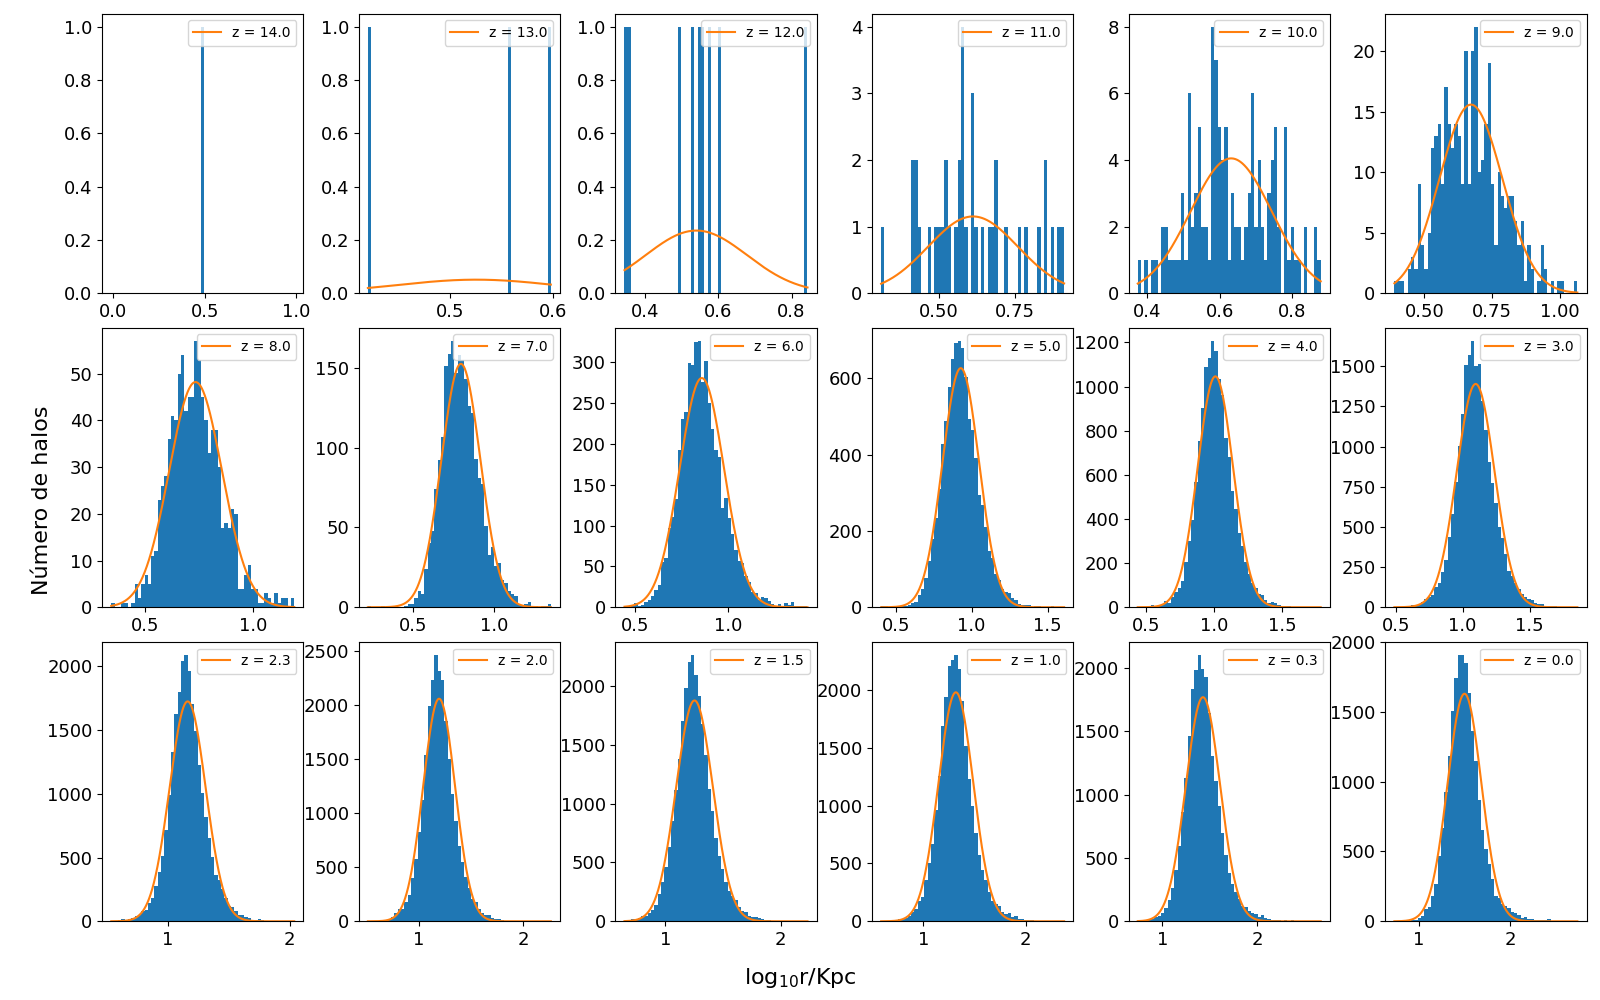
\includegraphics[width = 0.75\linewidth]{RunInvertida/HalfMassRad_Dist_RunInvertidaSep.png}
    \caption[Radio que contiene la mitad de la masa]{\footnotesize Mostramos la cantidad de halos de materia oscura en los diferentes rangos del radio que contiene la mitad de la masa y su ajuste conforme evoluciona en el Universo $\Omega_\lambda = 0.309 $, $\Omega_0 = 0.691$. Se muestran las distribuciones empezando en $z=14$ en la parte superior izquierda y terminado en $z=0$ en la parte inferior derecha.}
    \label{fig:Invertida-HalfMassRadDistSep}
\end{figure}

\begin{figure}[H]
    \centering
    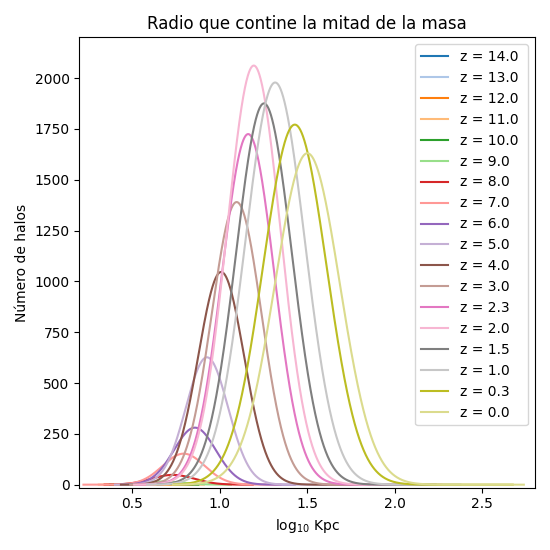
\includegraphics[width = 0.5\linewidth]{RunInvertida/HalfMassRad_Dist_RunInvertida.png}
    \caption[Distribución del Radio que contiene la mitad de la masa]{\footnotesize Mostramos los ajustes de la figura \ref{fig:Invertida-HalfMassRadDistSep} para destacar la evolución de la distribución del radio que contiene la mitad de la masa del Universo $\Omega_\lambda = 0.309 $, $\Omega_0 = 0.691$ desde un $z=14$ hasta un $z=0$.}
    \label{fig:Invertida-HalfMassRadDist}
\end{figure}

\begin{figure}[H]
    \centering
    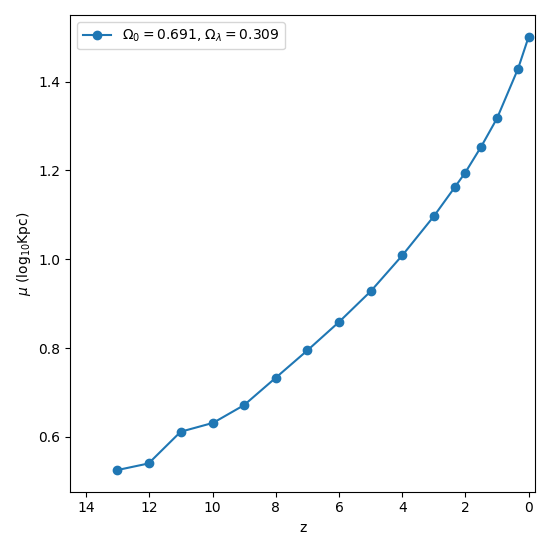
\includegraphics[width = 0.4\linewidth]{RunInvertida/HalfMassRad_Mean_RunInvertida.png}
    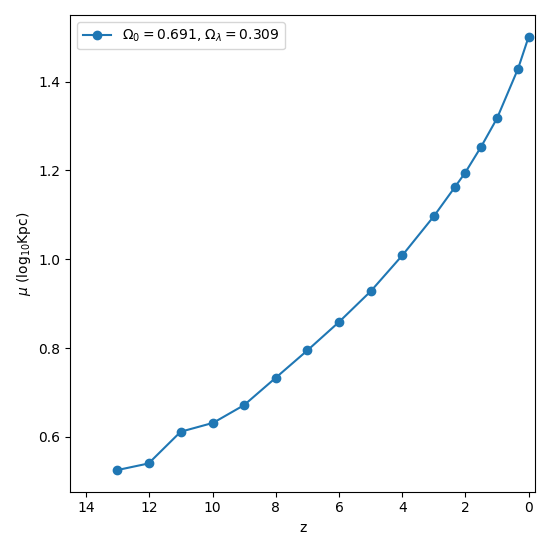
\includegraphics[width = 0.4\linewidth]{RunInvertida/HalfMassRad_Std_RunInvertida.png}
    \caption[Media y desviación estándar del radio de la mitad de la masa]{\footnotesize En la izquierda mostramos la media del radio que contiene la mitad de la masa de los halos de materia oscura donde observamos como cambian durante la evolución del Universo. En la derecha se muestra la desviación estándar del radio que contiene la mitad de la masa que nos muestra la variedad de halos que hay durante la evolución del Universo, desde un $z=14$ hasta un $z=0$.}
    \label{fig:Invertida-HalfMassRadStats}
\end{figure}

Ahora veamos el comportamiento del radio asociado con la velocidades circular. En las figuras \ref{fig:Invertida-VMaxRadDistSep} y \ref{fig:Invertida-VMaxRadDist} observamos que a lo largo de la evolución de las estructuras tenemos halos con radios que van desde los $4.29$ kpc hasta los $568.53$ kpc. Vemos que la gran mayoría de los halos con tamaños entre $11.79$ kpc y $49.25$ kpc en $z=0$ y entre $4.29$ kpc y $4.31$ kpc en $z=13$. En la figura \ref{fig:Invertida-VMaxRadStats} vemos que la media va desde los $4.28$ kpc con una desviación de $0.03$ kpc en $z=13$ hasta $30.52$ kpc con una desviación de $18.73$ kpc en $z=0$.

\begin{figure}[H]
    \centering
    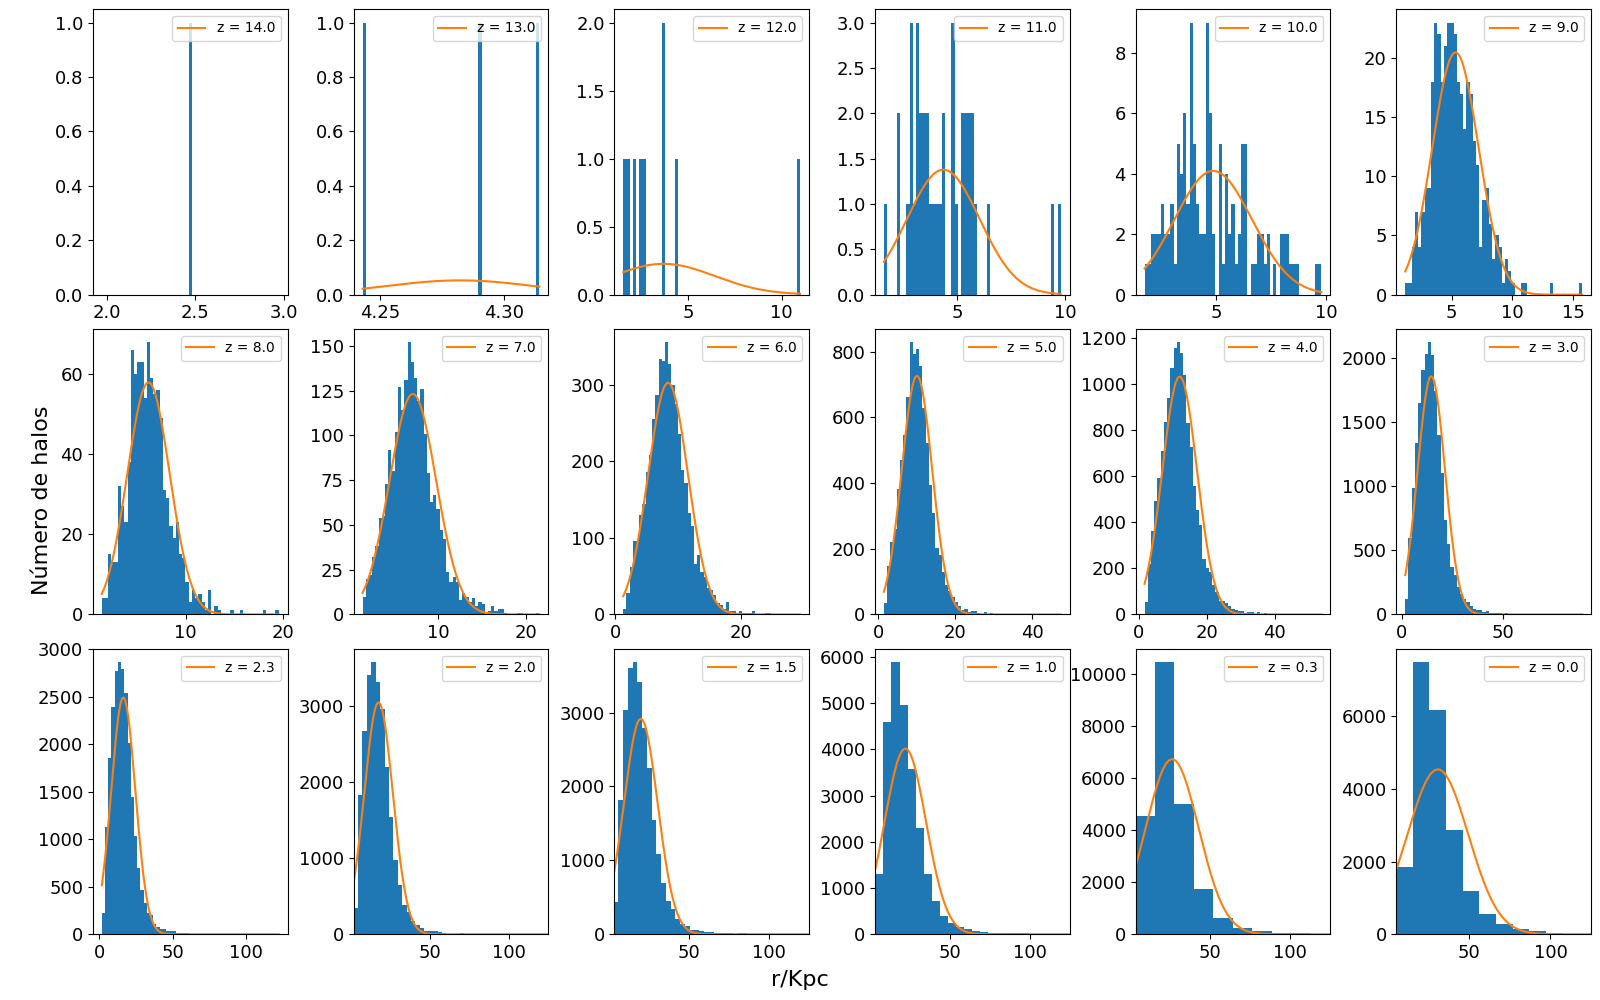
\includegraphics[width = 0.75\linewidth]{RunInvertida/VMaxRad_Dist_RunInvertidaSep.png}
    \caption[Radio donde se alcanza la velocidad máxima circular]{\footnotesize Mostramos la cantidad de halos de materia oscura en los diferentes rangos del radio donde alcanza su velocidad máxima circular y su ajuste conforme evoluciona en el Universo $\Omega_\lambda = 0.309 $, $\Omega_0 = 0.691$. Se muestran las distribuciones empezando en $z=14$ en la parte superior izquierda y terminado en $z=0$ en la parte inferior derecha.}
    \label{fig:Invertida-VMaxRadDistSep}
\end{figure}

\begin{figure}[H]
    \centering
    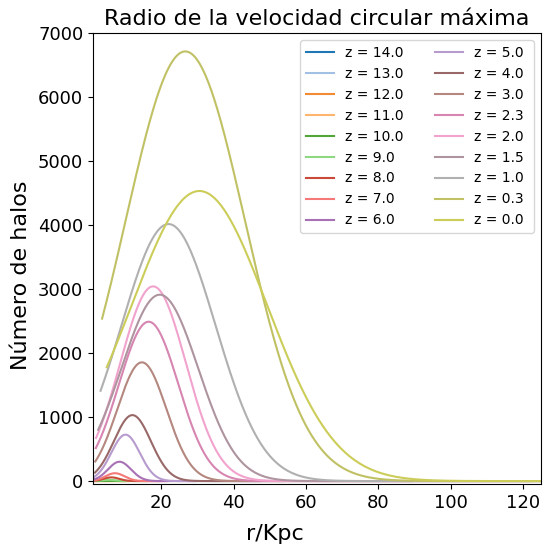
\includegraphics[width = 0.5\linewidth]{RunInvertida/VMaxRad_Dist_RunInvertida.png}
    \caption[Distribución del radio donde se alcanza la velocidad máxima circular]{\footnotesize Mostramos los ajustes de la figura \ref{fig:Invertida-VMaxRadDistSep} para destacar la evolución de la distribución del radio donde alcanza su velocidad máxima circular del Universo $\Omega_\lambda = 0.309 $, $\Omega_0 = 0.691$ desde un $z=14$ hasta un $z=0$.}
    \label{fig:Invertida-VMaxRadDist}
\end{figure}

\begin{figure}[H]
    \centering
    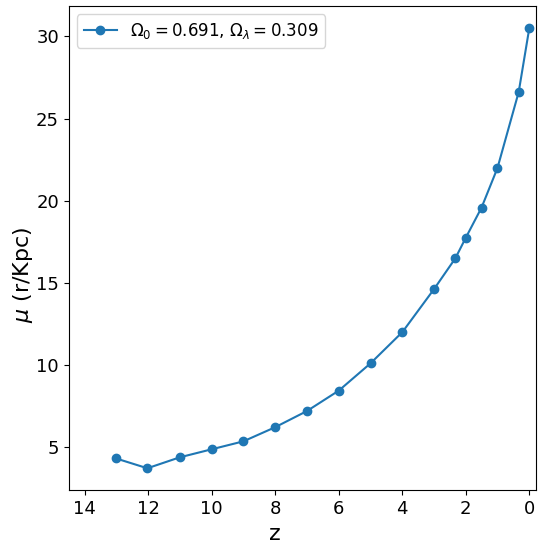
\includegraphics[width = 0.4\linewidth]{RunInvertida/VMaxRad_Mean_RunInvertida.png}
    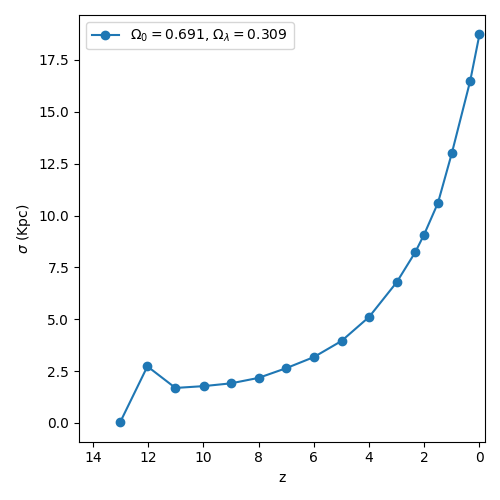
\includegraphics[width = 0.4\linewidth]{RunInvertida/VMaxRad_Std_RunInvertida.png}
    \caption[Media y desviación estándar del Radio donde se alcanza la velocidad máxima circular]{\footnotesize En la izquierda mostramos la media del radio donde alcanza su velocidad máxima circular en los halos de materia oscura donde observamos como cambian durante la evolución del Universo. En la derecha se muestra la desviación estándar del radio donde alcanza su velocidad máxima circular que nos muestra la variedad de halos que hay durante la evolución del Universo, desde un $z=14$ hasta un $z=0$.}
    \label{fig:Invertida-VMaxRadStats}
\end{figure}

Seguimos con la velocidad circular máxima. De las figuras \ref{fig:Invertida-VelMaxDistSep} y \ref{fig:Invertida-VelMaxDist} apreciamos que las velocidades circulares están en el rangos de $33.10$ kms$^{-1}$ hasta los $1370.96$ kms$^{-1}$ donde vemos la gran mayoría de los halos en los rangos de $58.72$ kms$^{-1}$ y $153.42$ kms$^{-1}$ en $z=0$, mientras que en $z=13$ estos se encuentran entre $190.29$ kms$^{-1}$ y $223.92$ kms$^{-1}$. En la figura \ref{fig:Invertida-VelMaxStats} apreciamos como la velocidad media disminuye rápidamente desde $207.02$ kms$^{-1}$ con una desviación de $13.72$ kms$^{-1}$ en $z=13$ hasta que alcanza $106.07$ kms$^{-1}$ con una desviación de $47.35$ kms$^{-1}$ en $z=0$. 

\begin{figure}[H]
    \centering
    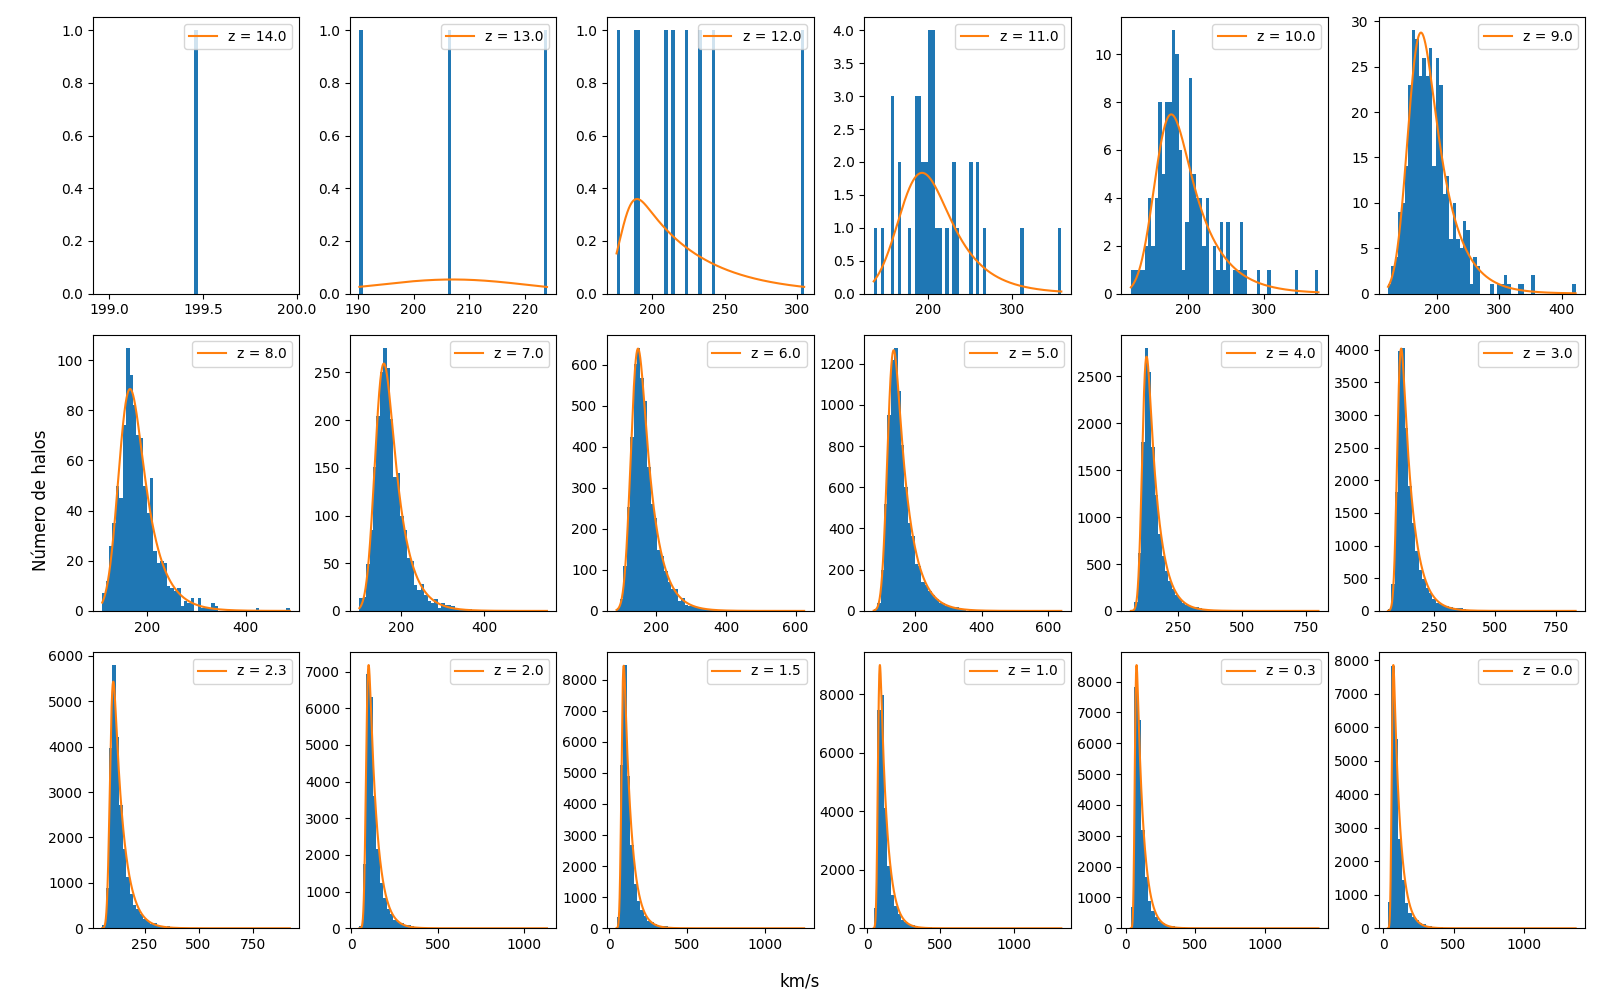
\includegraphics[width = 0.75\linewidth]{RunInvertida/VelMax_Dist_RunInvertidaSep.png}
    \caption[Velocidad circular máxima]{\footnotesize Mostramos la cantidad de halos de materia oscura en los diferentes rangos de la velocidad circular máxima y su ajuste conforme evoluciona en el Universo $\Omega_\lambda = 0.309 $, $\Omega_0 = 0.691$. Se muestran las distribuciones empezando en $z=14$ en la parte superior izquierda y terminado en $z=0$ en la parte inferior derecha.}
    \label{fig:Invertida-VelMaxDistSep}
\end{figure}

\begin{figure}[H]
    \centering
    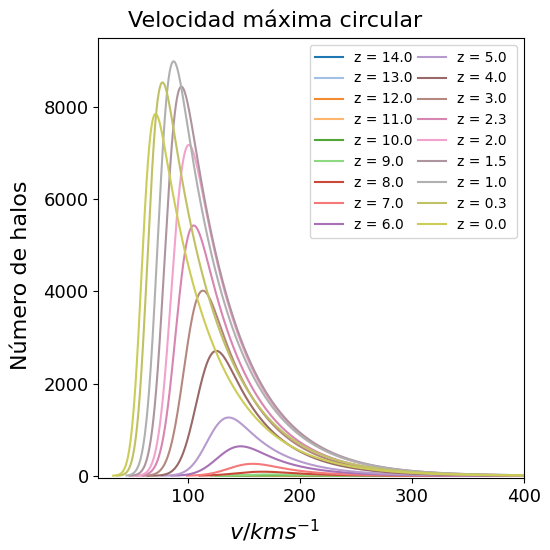
\includegraphics[width = 0.5\linewidth]{RunInvertida/VelMax_Dist_RunInvertida.png}
    \caption[Distribución de la velocidad circular máxima]{\footnotesize Mostramos los ajustes de la figura \ref{fig:Invertida-VelMaxDistSep} para destacar la evolución de la distribución de la velocidad circular máxima del Universo $\Omega_\lambda = 0.309 $, $\Omega_0 = 0.691$ desde un $z=14$ hasta un $z=0$.}
    \label{fig:Invertida-VelMaxDist}
\end{figure}

\begin{figure}[H]
    \centering
    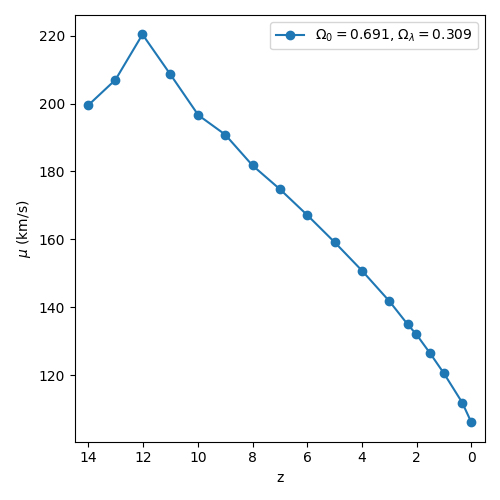
\includegraphics[width = 0.4\linewidth]{RunInvertida/VelMax_Mean_RunInvertida.png}
    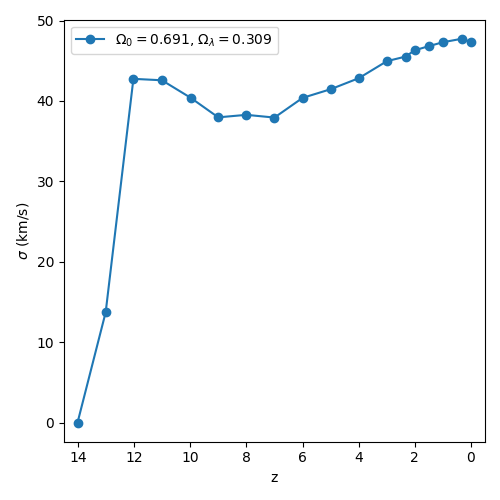
\includegraphics[width = 0.4\linewidth]{RunInvertida/VelMax_Std_RunInvertida.png}
    \caption[Media y desviación estándar de la velocidad circular máxima]{\footnotesize En la izquierda mostramos la media de la velocidad circular máxima en los halos de materia oscura donde observamos como cambian durante la evolución del Universo. En la derecha se muestra la desviación estándar de la velocidad circular máxima que nos muestra la variedad de halos que hay durante la evolución del Universo, desde un $z=14$ hasta un $z=0$.}
    \label{fig:Invertida-VelMaxStats}
\end{figure}

Continuando con la dispersión de velocidades. De las figuras \ref{fig:Invertida-VelDispDistSep} y \ref{fig:Invertida-VelDispDist} vemos que las velocidades varían entre $17.06$ kms$^{-1}$ y $810.69$ kms$^{-1}$ a lo largo del Universo, donde en $z=13$ tenemos que las velocidades alcanzan entre $102.23$ kms$^{-1}$ y $126.98$ kms$^{-1}$ y en $z=0$ la mayoría de los tienen velocidades entre $27.32$ kms$^{-1}$ y $80.74$ kms$^{-1}$ con un máximo en $810.69$ kms$^{-1}$. En la figura \ref{fig:Invertida-VelDispStats} observamos que la dispersión de velocidades media disminuye desde los $116.20$ kms$^{-1}$ con una desviación de $10.35$ kms$^{-1}$ en $z=13$ a $54.03$ kms$^{-1}$ con una desviación de $26.71$ kms$^{-1}$ en $z=0$.

\begin{figure}[H]
    \centering
    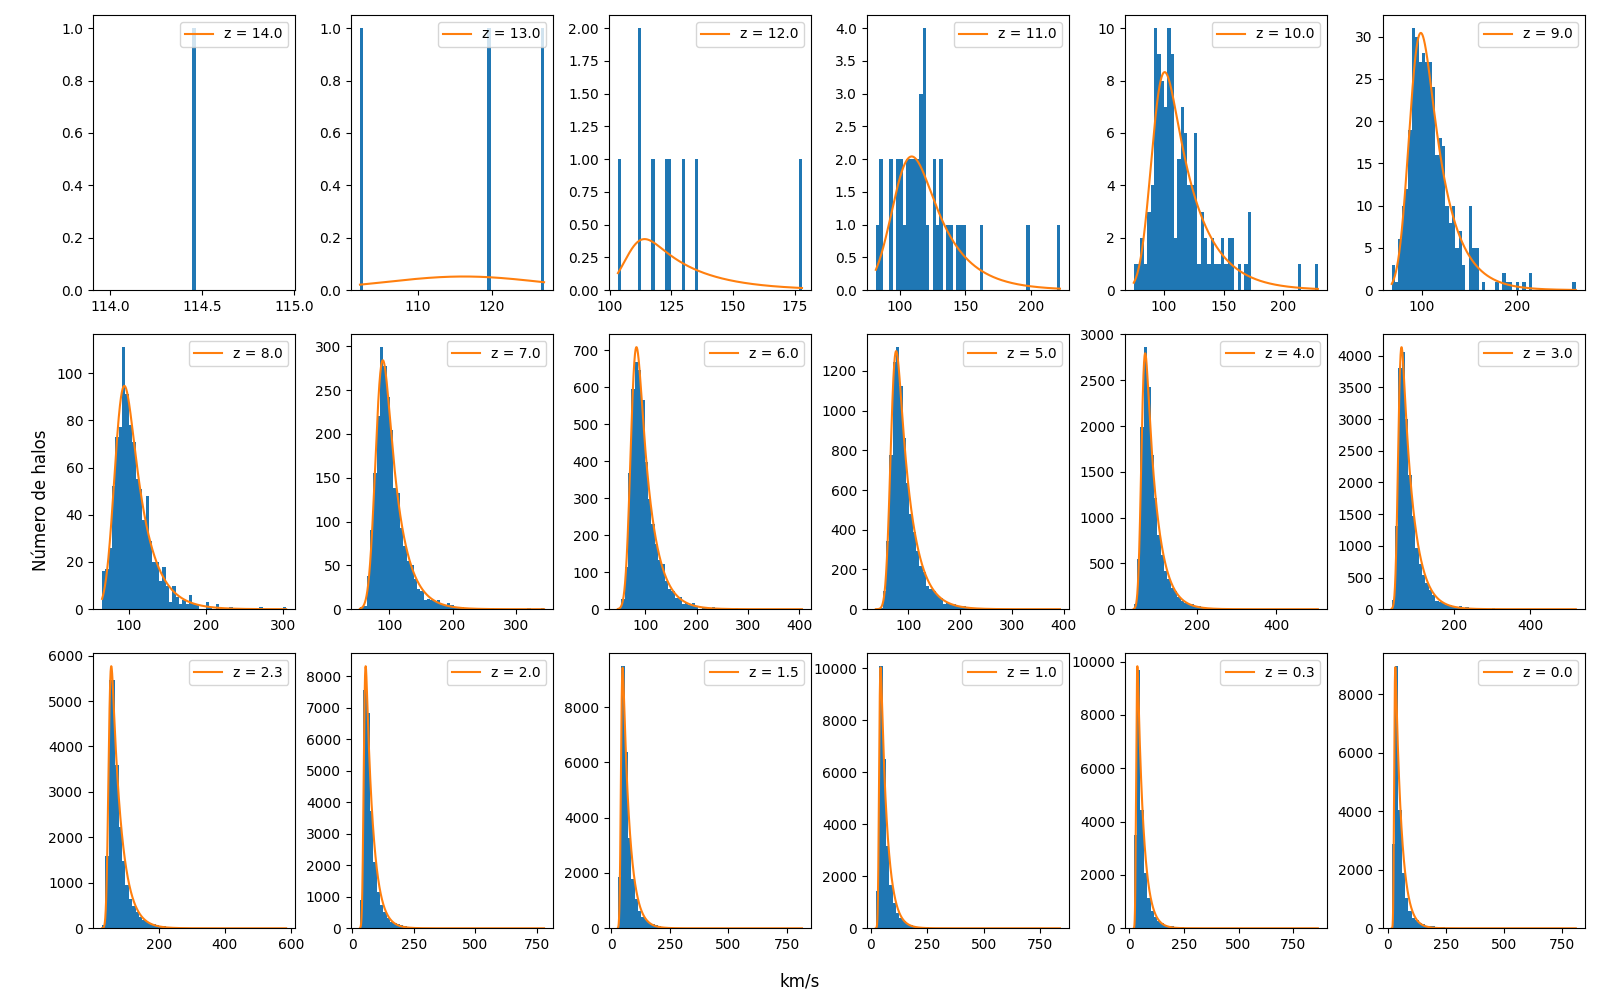
\includegraphics[width = 0.75\linewidth]{RunInvertida/VelDisp_Dist_RunInvertidaSep.png}
    \caption[Dispersión de velocidades]{\footnotesize Mostramos la cantidad de halos en los diferentes rangos de la dispersión de velocidades y su ajuste conforme evoluciona el Universo $\Omega_\lambda = 0.309 $, $\Omega_0 = 0.691$. Se muestran las distribuciones empezando en $z=14$ en la parte superior izquierda y terminando en $z=0$ en la parte inferior derecha.}
    \label{fig:Invertida-VelDispDistSep}
\end{figure}

\begin{figure}[H]
    \centering
    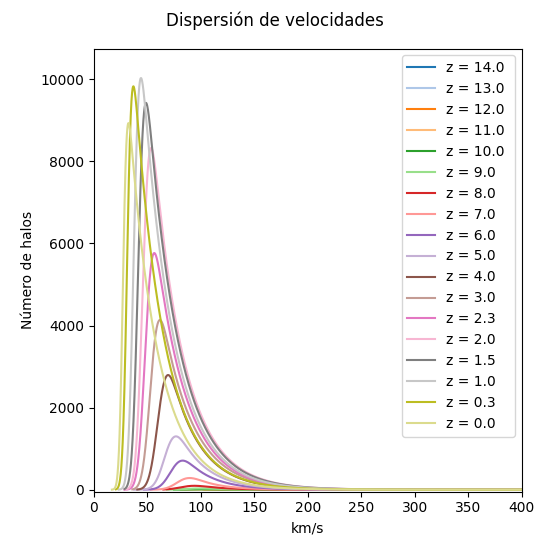
\includegraphics[width = 0.5\linewidth]{RunInvertida/VelDisp_Dist_RunInvertida.png}
    \caption[Distribución de la dispersión de velocidades]{\footnotesize Mostramos los ajustes de la figura \ref{fig:Invertida-VelDispDistSep} para destacar la evolución de la distribución de la dispersión de velocidades del Universo $\Omega_\lambda = 0.309 $, $\Omega_0 = 0.691$ desde un $z=14$ hasta un $z=0$.}
    \label{fig:Invertida-VelDispDist}
\end{figure}

\begin{figure}[H]
    \centering
    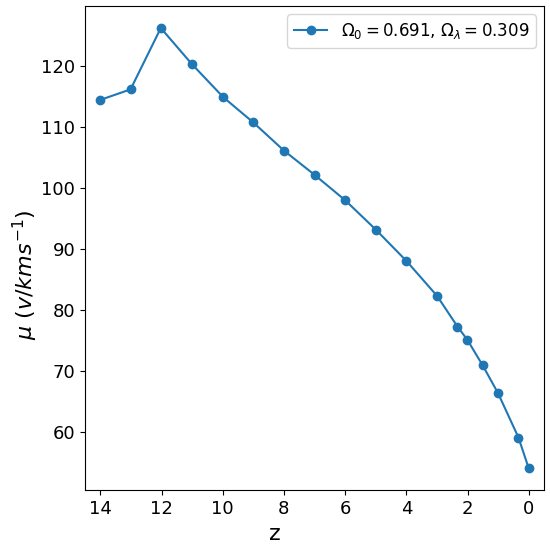
\includegraphics[width = 0.4\linewidth]{RunInvertida/VelDisp_Mean_RunInvertida.png}
    \includegraphics[width = 0.4\linewidth]{RunInvertida/VelDisp_Std_RunInvertida.png}
    \caption[Media y desviación estándar de la dispersión de velocidades]{\footnotesize En la izquierda mostramos la media de la dispersión de velocidades en los halos de materia oscura donde observamos como cambian durante la evolución del Universo. En la derecha se muestra la desviación estándar de la dispersión de velocidades que nos muestra la variedad de halos que hay durante la evolución del Universo, desde un $z=14$ hasta un $z=0$.}
    \label{fig:Invertida-VelDispStats}
\end{figure}

La figura \ref{fig:Invertida-DensityMap} muestra el mapa de densidad de un Universo $\Omega_\lambda = 0.309 $ $\Omega_0 = 0.691$, donde podemos ver la estructura que describimos en los diferentes puntos de su evolución vista desde un plano.

\begin{figure}[H]
    \centering

    \includegraphics[width = 0.33\linewidth]{RunInvertida/RunInvertidaZ63.png}   %snap 000 z=63
    \includegraphics[width = 0.33\linewidth]{RunInvertida/RunInvertidaZ25.png}   %snap 005 z=25
    \includegraphics[width = 0.32\linewidth]{RunInvertida/RunInvertidaZ20.png}   %snap 010 z=20
    \\
    \includegraphics[width = 0.33\linewidth]{RunInvertida/RunInvertidaZ15.png}   %snap 015 z=15
    \includegraphics[width = 0.33\linewidth]{RunInvertida/RunInvertidaZ10.png}   %snap 020 z=10
    \includegraphics[width = 0.32\linewidth]{RunInvertida/RunInvertidaZ5.png}    %snap 025 z=5
    \\
    \includegraphics[width = 0.33\linewidth]{RunInvertida/RunInvertidaZ3.png}    %snap 027 z=3
    \includegraphics[width = 0.33\linewidth]{RunInvertida/RunInvertidaZ1_5.png}  %snap 030 z=1.5
    \includegraphics[width = 0.32\linewidth]{RunInvertida/RunInvertidaZ0.png}    %snap 033 z=0
    \caption[Mapa de densidad en en diferentes redshift]{ \footnotesize Mapa de densidad de la simulación en diferentes redshifts de una cosmología $\Omega_\lambda = 0.309 $, $\Omega_0 = 0.691$. }
    \label{fig:Invertida-DensityMap}
\end{figure}

%====================================================================================================================
%=====================================  RUN HALF COSMO  =============================================================
%====================================================================================================================
\subsection{Universo con cosmología \texorpdfstring{$\Omega_\lambda = 0.5$, $\Omega_0 = 0.5$ }{Omega lambda = 0.5, Omega 0 = 0.5} }

Hemos visto que como se comporta un Universo con las densidades más aceptadas y cuando estas se invierten. Ahora veamos un Universo con las densidades iguales ($\Omega_\lambda = 0.5$, $\Omega_0 = 0.5$). Comencemos viendo como se afecta la cantidad de halos. La figura \ref{fig:HalfCosmo-TotalHalos} muestra que los primeros halos aparecen en $z=15$, además vemos que el máximo de halos se alcanza fue de $26242$ halos en $z=1.5$. Apreciamos un comportamiento similar a las cosmologías anteriores donde vemos un crecimiento rápido hasta que alcanza un máximo y después empieza a disminuir.

\begin{figure}[H]
    \centering
    \includegraphics[scale = 0.5]{RunHalfCosmo/TotalHalos_RunHalfCosmo.png}
    \caption[Evolución del número de halos en un Universo $\Omega_\lambda = 0.5 $, $\Omega_0 = 0.5$]{\footnotesize Se muestra el número de halos y como cambia la cantidad conforme evoluciona el Universo en una cosmología $\Omega_\lambda = 0.5 $ y $\Omega_0 = 0.5$.}    
    \label{fig:HalfCosmo-TotalHalos}
\end{figure}

La distribución de la masa para esta cosmología se observa en las figuras \ref{fig:HalfCosmo-MassDistSep} y \ref{fig:HalfCosmo-MassDist}. Los rangos de la masa se encuentran entre las $10^{10.32}$ $M_\odot$ a $10^{14.51}$ $M_\odot$ a lo largo de de la evolución del sistema. En $z=14$, los halos tenían masas menores a las $10^{10.75}$ $M_\odot$ y las estructuras en $z=0$ la mayor parte de los halos tenían masas entre $10^{10.47}$ $M_\odot$ y $10^{11.45}$ $M_\odot$. Mientras, la figura \ref{fig:HalfCosmo-MassStats} nos muestra el comportamiento medio durante la evolución, donde apreciamos que la masa media incrementa desde $10^{10.65}$ $M_\odot$ con una desviación de $10^{0.10}$ $M_\odot$ en $z=14$ hasta $10^{10.96}$ $M_\odot$ con una desviación de $10^{0.49}$ $M_\odot$ en $z=0$.

\begin{figure}[H]
    \centering
    \includegraphics[width = 0.8\linewidth]{RunHalfCosmo/Mass_Dist_RunHalfCosmoSep.png}
    \caption[Distribución de masa]{\footnotesize Mostramos la cantidad de halos en los diferentes rangos de masa y su ajuste conforme evoluciona el Universo en una cosmología $\Omega_\lambda = 0.5 $ y $\Omega_0 = 0.5$. Se muestran las distribuciones en los diferentes redshifts empezando en $z=15$ en la parte superior izquierda y terminado en $z=0$ en la parte inferior derecha. Se observa como aumentan la cantidad de halos cada vez más masivos.}
    \label{fig:HalfCosmo-MassDistSep}
\end{figure}

\begin{figure}[H]
    \centering
    \includegraphics[width = 0.5\linewidth]{RunHalfCosmo/Mass_Dist_RunHalfCosmo.png}
    \caption[Comparación de distribución de masa Universo]{\footnotesize Mostramos los ajustes de la figura \ref{fig:HalfCosmo-MassDistSep} para destacar la evolución de la distribución de masa del Universo $\Omega_\lambda = 0.5$, $\Omega_0 = 0.5$ desde un $z=15$ hasta un $z=0$.}
    \label{fig:HalfCosmo-MassDist}
\end{figure}

\begin{figure}[H]
    \centering
    \includegraphics[width = 0.4\linewidth]{RunHalfCosmo/MassMean_RunHalfCosmo.png}
    \includegraphics[width = 0.4\linewidth]{RunHalfCosmo/MassStd_RunHalfCosmo.png}
    \caption[Media y desviación estándar de la distribución de masa]{\footnotesize En la izquierda se muestra la masa media de los halos de materia oscura donde observamos como cambian durante la evolución del Universo. En la derecha se muestra la desviación estándar de la masa, la cual nos muestra la variedad de los halos que hay durante la evolución del Universo, desde un $z=15$ hasta un $z=0$.}
    \label{fig:HalfCosmo-MassStats}
\end{figure}

En las figuras \ref{fig:HalfCosmo-HalfMassRadDistSep} y \ref{fig:HalfCosmo-HalfMassRadDist} podemos ver el radio que contiene la mitad de la masa de los halos a lo largo de la evolución del Universo. Vemos que los radios se encuentran entre los $10^{0.40}$ kpc y $10^{2.72}$ kpc a lo largo de la evolución del sistema, donde los halos en $z=14$ tienen radios entre los $10^{0.40}$ kpc y los $10^{0.61}$ y las estructuras $z=0$ tienen la mayor parte de los halos en el rango de $10^{1.31}$ kpc y los $10^{1.67}$. En la figura \ref{fig:HalfCosmo-HalfMassRadStats} apreciamos que el radio medio tiene un crecimiento de $10^{0.53}$ kpc con una desviación de $10^{0.09}$ kpc en $z=14$ hasta un radio de $10^{1.49}$ kpc con una desviación de $10^{0.18}$ kpc en $z=0$.

\begin{figure}[H]
    \centering
    \includegraphics[width = 0.75\linewidth]{RunHalfCosmo/HalfMassRad_Dist_RunHalfCosmoSep.png}
    \caption[Radio que contiene la mitad de la masa]{\footnotesize Mostramos la cantidad de halos de materia oscura en los diferentes rangos del radio que contiene la mitad de la masa y su ajuste conforme evoluciona en el Universo $\Omega_\lambda = 0.5 $, $\Omega_0 = 0.5$. Se muestran las distribuciones empezando en $z=15$ en la parte superior izquierda y terminado en $z=0$ en la parte inferior derecha.}
    \label{fig:HalfCosmo-HalfMassRadDistSep}
\end{figure}

\begin{figure}[H]
    \centering
    \includegraphics[width = 0.5\linewidth]{RunHalfCosmo/HalfMassRad_Dist_RunHalfCosmo.png}
    \caption[Distribución del Radio que contiene la mitad de la masa]{\footnotesize Mostramos los ajustes de la figura \ref{fig:HalfCosmo-HalfMassRadDistSep} para destacar la evolución de la distribución del radio que contiene la mitad de la masa del Universo $\Omega_\lambda = 0.5 $, $\Omega_0 = 0.5$ desde un $z=15$ hasta un $z=0$.}
    \label{fig:HalfCosmo-HalfMassRadDist}
\end{figure}

\begin{figure}[H]
    \centering
    \includegraphics[width = 0.4\linewidth]{RunHalfCosmo/HalfMassRad_Mean_RunHalfCosmo.png}
    \includegraphics[width = 0.4\linewidth]{RunHalfCosmo/HalfMassRad_Std_RunHalfCosmo.png}
    \caption[Media y desviación estándar del radio de la mitad de la masa]{\footnotesize En la izquierda mostramos la media del radio que contiene la mitad de la masa de los halos de materia oscura donde observamos como cambian durante la evolución del Universo. En la derecha se muestra la desviación estándar del radio que contiene la mitad de la masa que nos muestra la variedad de halos que hay durante la evolución del Universo, desde un $z=14$ hasta un $z=0$.}
    \label{fig:HalfCosmo-HalfMassRadStats}
\end{figure}

Ahora veamos el comportamiento del radio asociado con la velocidades circular. En las figuras \ref{fig:HalfCosmo-VMaxRadDistSep} y \ref{fig:HalfCosmo-VMaxRadDist} observamos que a lo largo de la evolución de las estructuras, tenemos halos con radios que van desde los $1.78$ kpc hasta los $593.77$ kpc. Vemos que los halos tienen radios menores a $4.61$ kpc en $z=14$ y en $z=0$ se encuentran entre $11.48$ kpc y $47.40$ kpc. En la figura \ref{fig:HalfCosmo-VMaxRadStats} vemos que la media va desde los $3.39$ kpc con una desviación de $1.19$ kpc en $z=14$ hasta $29.44$ kpc con una desviación de $17.96$ kpc en $z=0$.

\begin{figure}[H]
    \centering
    \includegraphics[width = 0.75\linewidth]{RunHalfCosmo/VMaxRad_Dist_RunHalfCosmoSep.png}
    \caption[Radio donde se alcanza la velocidad máxima circular]{\footnotesize Mostramos la cantidad de halos de materia oscura en los diferentes rangos del radio donde alcanza su velocidad máxima circular y su ajuste conforme evoluciona en el Universo $\Omega_\lambda = 0.5$, $\Omega_0 = 0.5$. Se muestran las distribuciones empezando en $z=15$ en la parte superior izquierda y terminado en $z=0$ en la parte inferior derecha.}
    \label{fig:HalfCosmo-VMaxRadDistSep}
\end{figure}

\begin{figure}[H]
    \centering
    \includegraphics[width = 0.5\linewidth]{RunHalfCosmo/VMaxRad_Dist_RunHalfCosmo.png}
    \caption[Distribución del radio donde se alcanza la velocidad máxima circular]{\footnotesize Mostramos los ajustes de la figura \ref{fig:HalfCosmo-VMaxRadDistSep} para destacar la evolución de la distribución del radio donde alcanza su velocidad máxima circular del Universo $\Omega_\lambda = 0.5$, $\Omega_0 = 0.5$ desde un $z=15$ hasta un $z=0$.}
    \label{fig:HalfCosmo-VMaxRadDist}
\end{figure}

\begin{figure}[H]
    \centering
    \includegraphics[width = 0.4\linewidth]{RunHalfCosmo/VMaxRad_Mean_RunHalfCosmo.png}
    \includegraphics[width = 0.4\linewidth]{RunHalfCosmo/VMaxRad_Std_RunHalfCosmo.png}
    \caption[Media y desviación estándar del Radio donde se alcanza la velocidad máxima circular]{\footnotesize En la izquierda mostramos la media del radio donde alcanza su velocidad máxima circular en los halos de materia oscura donde observamos como cambian durante la evolución del Universo. En la derecha se muestra la desviación estándar del radio donde alcanza su velocidad máxima circular que nos muestra la variedad de halos que hay durante la evolución del Universo, desde un $z=15$ hasta un $z=0$.}
    \label{fig:HalfCosmo-VMaxRadStats}
\end{figure}

Seguimos con la velocidad circular máxima que se alcanza en estos radios. De las figuras\ref{fig:HalfCosmo-VelDispDistSep} y \ref{fig:HalfCosmo-VelDispDist} apreciamos que las velocidades circulares están en el rangos de $26.01$ kms$^{-1}$ y $1196.36$ kms$^{-1}$ a lo largo de la evolución. En $z=14$ tenemos halos con velocidades entre $167.90$ kms$^{-1}$ y $183.73$ kms$^{-1}$ y en $z=0$ la mayoría se encuentran entre $50.85$ kms$^{-1}$ y $133.45$ kms$^{-1}$. En la figura \ref{fig:HalfCosmo-VelMaxStats} observamos que la velocidad media disminuye rápidamente desde $177.21$ kms$^{-1}$ con una desviación de $6.76$ kms$^{-1}$ en $z=14$ hasta que alcanza $92.15$ kms$^{-1}$ con una desviación de $41.30$ kms$^{-1}$ en $z=0$. 

\begin{figure}[H]
    \centering
    \includegraphics[width = 0.75\linewidth]{RunHalfCosmo/VelMax_Dist_RunHalfCosmoSep.png}
    \caption[Velocidad circular máxima]{\footnotesize Mostramos la cantidad de halos de materia oscura en los diferentes rangos de la velocidad circular máxima y su ajuste conforme evoluciona en el Universo $\Omega_\lambda = 0.5$, $\Omega_0 = 0.5$. Se muestran las distribuciones empezando en $z=15$ en la parte superior izquierda y terminado en $z=0$ en la parte inferior derecha.}
    \label{fig:HalfCosmo-VelMaxDistSep}
\end{figure}

\begin{figure}[H]
    \centering
    \includegraphics[width = 0.5\linewidth]{RunHalfCosmo/VelMax_Dist_RunHalfCosmo.png}
    \caption[Distribución de la velocidad circular máxima]{\footnotesize Mostramos los ajustes de la figura \ref{fig:HalfCosmo-VelMaxDistSep} para destacar la evolución de la distribución de la velocidad circular máxima del Universo $\Omega_\lambda = 0.5$, $\Omega_0 = 0.5$ desde un $z=15$ hasta un $z=0$.}
    \label{fig:HalfCosmo-VelMaxDist}
\end{figure}

\begin{figure}[H]
    \centering
    \includegraphics[width = 0.4\linewidth]{RunHalfCosmo/VelMax_Mean_RunHalfCosmo.png}
    \includegraphics[width = 0.4\linewidth]{RunHalfCosmo/VelMax_Std_RunHalfCosmo.png}
    \caption[Media y desviación estándar de la velocidad circular máxima]{\footnotesize En la izquierda mostramos la media de la velocidad circular máxima en los halos de materia oscura donde observamos como cambian durante la evolución del Universo. En la derecha se muestra la desviación estándar de la velocidad circular máxima que nos muestra la variedad de halos que hay durante la evolución del Universo, desde un $z=15$ hasta un $z=0$.}
    \label{fig:HalfCosmo-VelMaxStats}
\end{figure}

Continuando con la dispersión de velocidades, de las figuras \ref{fig:HalfCosmo-VelDispDistSep} y \ref{fig:HalfCosmo-VelDispDist} vemos que la dispersión se encentra entre $14.33$ kms$^{-1}$ y $702.94$ kms$^{-1}$ a lo largo de la evolución de los halos. En $z=14$ los halos tienen velocidades entre $89.36$ kms$^{-1}$ y $110.83$ kms$^{-1}$ y en $z=0$ la mayoría de las velocidades se encuentran entre $23.31$ kms$^{-1}$ y $69.57$ kms$^{-1}$ con halos que alcanzan los $702.94$ kms$^{-1}$. En la figura \ref{fig:HalfCosmo-VelDispStats} observamos que la dispersión de velocidades media disminuye desde los $102.29$ kms$^{-1}$ con una desviación de $9.32$ kms$^{-1}$ en $z=14$ a $46.44$ kms$^{-1}$ con una desviación de $23.13$ kms$^{-1}$ en $z=0$.

\begin{figure}[H]
    \centering
    \includegraphics[width = 0.75\linewidth]{RunHalfCosmo/VelDisp_Dist_RunHalfCosmoSep.png}
    \caption[Dispersión de velocidades]{\footnotesize Mostramos la cantidad de halos en los diferentes rangos de la dispersión de velocidades y su ajuste conforme evoluciona el Universo $\Omega_\lambda = 0.5$, $\Omega_0 = 0.5$. Se muestran las distribuciones empezando en $z=15$ en la parte superior izquierda y terminando en $z=0$ en la parte inferior derecha.}
    \label{fig:HalfCosmo-VelDispDistSep}
\end{figure}

\begin{figure}[H]
    \centering
    \includegraphics[width = 0.5\linewidth]{RunHalfCosmo/VelDisp_Dist_RunHalfCosmo.png}
    \caption[Distribución de la dispersión de velocidades]{\footnotesize Mostramos los ajustes de la figura \ref{fig:HalfCosmo-VelDispDistSep} para destacar la evolución de la distribución de la dispersión de velocidades del Universo $\Omega_\lambda = 0.5$, $\Omega_0 = 0.5$ desde un $z=15$ hasta un $z=0$.}
    \label{fig:HalfCosmo-VelDispDist}
\end{figure}

\begin{figure}[H]
    \centering
    \includegraphics[width = 0.4\linewidth]{RunHalfCosmo/VelDisp_Mean_RunHalfCosmo.png}
    \includegraphics[width = 0.4\linewidth]{RunHalfCosmo/VelDisp_Std_RunHalfCosmo.png}
    \caption[Media y desviación estándar de la dispersión de velocidades]{\footnotesize En la izquierda mostramos la media de la dispersión de velocidades en los halos de materia oscura donde observamos como cambian durante la evolución del Universo. En la derecha se muestra la desviación estándar de la dispersión de velocidades que nos muestra la variedad de halos que hay durante la evolución del Universo, desde un $z=15$ hasta un $z=0$.}
    \label{fig:HalfCosmo-VelDispStats}
\end{figure}

La figura \ref{fig:HalfCosmo-DensityMap} muestra el mapa de densidad de un Universo $\Omega_\lambda = 0.5 $ $\Omega_0 = 0.5$, donde podemos ver la estructura que describimos en los diferentes puntos de su evolución vista desde un plano.
\begin{figure}[H]
    \centering

    \includegraphics[width = 0.33\linewidth]{RunHalfCosmo/RunHalfCosmoZ63.png}   %snap 000 z=63
    \includegraphics[width = 0.33\linewidth]{RunHalfCosmo/RunHalfCosmoZ25.png}   %snap 005 z=25
    \includegraphics[width = 0.32\linewidth]{RunHalfCosmo/RunHalfCosmoZ20.png}   %snap 010 z=20
    \\
    \includegraphics[width = 0.33\linewidth]{RunHalfCosmo/RunHalfCosmoZ15.png}   %snap 015 z=15
    \includegraphics[width = 0.33\linewidth]{RunHalfCosmo/RunHalfCosmoZ10.png}   %snap 020 z=10
    \includegraphics[width = 0.32\linewidth]{RunHalfCosmo/RunHalfCosmoZ5.png}    %snap 025 z=5
    \\
    \includegraphics[width = 0.33\linewidth]{RunHalfCosmo/RunHalfCosmoZ3.png}    %snap 027 z=3
    \includegraphics[width = 0.33\linewidth]{RunHalfCosmo/RunHalfCosmoZ1_5.png}  %snap 030 z=1.5
    \includegraphics[width = 0.32\linewidth]{RunHalfCosmo/RunHalfCosmoZ0.png}    %snap 033 z=0
    \caption[Mapa de densidad en en diferentes redshift]{ \footnotesize Mapa de densidad de la simulación en diferentes redshifts de una cosmología $\Omega_\lambda = 0.5$, $\Omega_0 = 0.5$. }
    \label{fig:HalfCosmo-DensityMap}
\end{figure}

%====================================================================================================================
%=====================================  Run Sub-Crítica  ============================================================
%====================================================================================================================
\section[Cosmología Sub-Crítica \texorpdfstring{$\Omega < 1$}{Omega < 1}]{Cosmología Sub-Crítica \texorpdfstring{$\Omega < 1$}{Omega < 1}}

\noindent Hemos visto los efectos en un Universo plano, ahora veamos tres nuevas cosmologías pero ahora son Universos abiertos acelerados, o bien un Universo Sub-Crítico. Estas nuevas cosmologías se eligieron de manera de obtener una idea de los efectos en el Universo cuando se altera una de sus densidad como se realizo anteriormente. Empezando con una cosmología donde las densidades son $\Omega_\lambda = 0$, $\Omega_0 = 0.309$, en este universo veremos los efectos de un Universo sin presencia de energía oscura. Luego pasaremos nuestra atención a estudiar los efectos de un Universo donde quitamos la mitad de la densidad de energía ($\Omega_\lambda = 0.3455$, $\Omega_0 = 0.309$) y para terminar con las cosmologías sub-críticas veremos los efectos en un Universo donde consideramos la mitad de la densidad de materia ($\Omega_\lambda = 0.5$, $\Omega_0 = 0.5$).

%====================================================================================================================
%====================================  Run No Dark Energy ===========================================================
%====================================================================================================================

\subsection{Universo con cosmología \texorpdfstring{$\Omega_\lambda = 0$, $\Omega_0 = 0.309$ }{Omega lambda = 0, Omega 0 = 0.309}  }

La primera cosmología que estudiaremos es en la que no hay efectos de la energía oscura. Lo primero que podemos observar en la figura \ref{fig:NoDE_TotalHalos} es que las estructuras se empiezan a formar a partir del redshift $z=25$. En $z= 2.33$ es donde alcanzamos la mayor cantidad halos. Alrededor de $z = 16$ es cuando empezamos a ver un crecimiento apreciable en la cantidad de halos.

\begin{figure}[H]
    \centering
    \includegraphics[scale = 0.5]{RunNoDE/TotalHalos_RunNoDE.png}
    \caption[Evolución del número de halos en un Universo $\Omega_\lambda = 0$, $\Omega_0 = 0.309$]{\footnotesize Se muestra el número de halos según el redshift y podemos observar como evoluciona el Universo en una cosmología $\Omega_\lambda = 0$ y $\Omega_0 = 0.309$.}
    \label{fig:NoDE_TotalHalos}
\end{figure}

La distribución de la masa para esta cosmología se observa en las figuras \ref{fig:NoDE-MassDistSep} y \ref{fig:NoDE-MassDist}. Los rangos de la masa se encuentran entre las $10^{10.11}$ $M_\odot$ a $10^{14.33}$ $M_\odot$ a lo largo de de la evolución del sistema. Las estructuras en $z=25$ tienen masas entre $10^{10.32}$ $M_\odot$ y $10^{10.62}$ $M_\odot$, mientras la mayoría de las estructuras en $z=0$ tienen la masa entre $10^{10.27}$ $M_\odot$ y $10^{11.25}$ $M_\odot$ con estructuras que alcanzan $10^{14.33}$ $M_\odot$. Mientras, en la figura \ref{fig:NoDE-MassStats} vemos que el comportamiento de la masa media incrementa desde $10^{10.42}$ $M_\odot$ con una desviación de $10^{0.10}$ $M_\odot$ en $z=25$ hasta $10^{10.76}$ $M_\odot$ con una desviación de $10^{0.49}$ $M_\odot$ en $z=0$.

\begin{figure}[H]
    \centering
    \includegraphics[width = 0.8\linewidth]{RunNoDE/Mass_Dist_RunNoDESep.png}
    \caption[Distribución de masa]{\footnotesize Mostramos la cantidad de halos en los diferentes rangos de masa y su ajuste conforme evoluciona el Universo en una cosmología $\Omega_\lambda = 0$ y $\Omega_0 = 0.309$. Se muestran las distribuciones en los diferentes redshifts empezando en $z=25$ en la parte superior izquierda y terminado en $z=0$ en la parte inferior derecha. Se observa como aumentan la cantidad de halos cada vez más masivos.}
    \label{fig:NoDE-MassDistSep}
\end{figure}

\begin{figure}[H]
    \centering
    \includegraphics[width = 0.5\linewidth]{RunNoDE/Mass_Dist_RunNoDE.png}
    \caption[Comparación de distribución de masa]{\footnotesize Mostramos los ajustes de la figura \ref{fig:NoDE-MassDistSep} para destacar la evolución de la distribución de masa del Universo $\Omega_\lambda = 0$, $\Omega_0 = 0.309$ desde un $z=25$ hasta un $z=0$.}
    \label{fig:NoDE-MassDist}
\end{figure}

\begin{figure}[H]
    \centering
    \includegraphics[width = 0.4\linewidth]{RunNoDE/MassMean_RunNoDE.png}
    \includegraphics[width = 0.4\linewidth]{RunNoDE/MassStd_RunNoDE.png}
    \caption[Media y desviación estándar de la distribución de masa]{\footnotesize En la izquierda se muestra la masa media de los halos de materia oscura donde observamos como cambian durante la evolución del Universo. En la derecha se muestra la desviación estándar de la masa, la cual nos muestra la variedad de los halos que hay durante la evolución del Universo, desde un $z=25$ hasta un $z=0$.}
    \label{fig:NoDE-MassStats}
\end{figure}

En las figuras \ref{fig:NoDE-HalfMassRadDistSep} y \ref{fig:NoDE-HalfMassRadDist} podemos ver el radio que contiene la mitad de la masa de los halos a lo largo de la evolución del Universo. Apreciamos que los radios se encuentran entre los $10^{0.09}$ kpc y $10^{2.57}$ kpc a lo largo de la evolución del sistema, donde los halos en $z=25$ tienen radios entre $10^{0.09}$ kpc y los $10^{0.43}$ y las estructuras en $z=0$ tienen la mayor parte de los halos en el rango de $10^{1.21}$ kpc y los $10^{1.57}$ kpc con halos que alcanzan hasta los $10^{2.57}$ kpc. En la figura \ref{fig:NoDE-HalfMassRadStats} vemos el crecimiento del radio medio desde $10^{0.32}$ kpc con una desviación de $10^{0.12}$ kpc en $z=25$ hasta un radio de $10^{1.39}$ kpc con una desviación de $10^{0.18}$ kpc en $z=0$.

\begin{figure}[H]
    \centering
    \includegraphics[width = 0.75\linewidth]{RunNoDE/HalfMassRad_Dist_RunNoDESep.png}
    \caption[Radio que contiene la mitad de la masa]{\footnotesize Mostramos la cantidad de halos de materia oscura en los diferentes rangos del radio que contiene la mitad de la masa y su ajuste conforme evoluciona en el Universo $\Omega_\lambda = 0$, $\Omega_0 = 0.309$. Se muestran las distribuciones empezando en $z=25$ en la parte superior izquierda y terminado en $z=0$ en la parte inferior derecha.}
    \label{fig:NoDE-HalfMassRadDistSep}
\end{figure}

\begin{figure}[H]
    \centering
    \includegraphics[width = 0.5\linewidth]{RunNoDE/HalfMassRad_Dist_RunNoDE.png}
    \caption[Distribución del radio que contiene la mitad de la masa]{\footnotesize Mostramos los ajustes de la figura \ref{fig:NoDE-HalfMassRadDistSep} para destacar la evolución de la distribución del radio que contiene la mitad de la masa del Universo $\Omega_\lambda = 0$, $\Omega_0 = 0.309$ desde un $z=25$ hasta un $z=0$.}
    \label{fig:NoDE-HalfMassRadDist}
\end{figure}

\begin{figure}[H]
    \centering
    \includegraphics[width = 0.4\linewidth]{RunNoDE/HalfMassRad_Mean_RunNoDE.png}
    \includegraphics[width = 0.4\linewidth]{RunNoDE/HalfMassRad_Std_RunNoDE.png}
    \caption[Media y desviación estándar del radio de la mitad de la masa]{\footnotesize En la izquierda mostramos la media del radio que contiene la mitad de la masa de los halos de materia oscura donde observamos como cambian durante la evolución del Universo. En la derecha se muestra la desviación estándar del radio que contiene la mitad de la masa que nos muestra la variedad de halos que hay durante la evolución del Universo, desde un $z=25$ hasta un $z=0$.}
    \label{fig:NoDE-HalfMassRadStats}
\end{figure}

Ahora veamos el comportamiento del radio asociado con la velocidades circular. En las figuras \ref{fig:NoDE-VMaxRadDistSep} y \ref{fig:NoDE-VMaxRadDist} observamos que a lo largo de la evolución de las estructuras, tenemos halos con radios que van desde los $1.28$ kpc hasta los $271.91$ kpc. Vemos que los halos tienen radios menores a $2.40$ kpc en $z=25$ y en $z=0$ la mayoría tienen radios entre $11.21$ kpc y $32.77$ kpc con algunos que alcanzan hasta $271.91$ kpc. En la figura \ref{fig:NoDE-VMaxRadStats} vemos que la media va desde los $1.76$ kpc con una desviación de $0.40$ kpc en $z=25$ hasta $21.99$ kpc con una desviación de $10.78$ kpc en $z=0$.

\begin{figure}[H]
    \centering
    \includegraphics[width = 0.75\linewidth]{RunNoDE/VMaxRad_Dist_RunNoDESep.png}
    \caption[Radio donde se alcanza la velocidad máxima circular]{\footnotesize Mostramos la cantidad de halos de materia oscura en los diferentes rangos del radio donde alcanza su velocidad máxima circular y su ajuste conforme evoluciona en el Universo $\Omega_\lambda = 0$, $\Omega_0 = 0.309$. Se muestran las distribuciones empezando en $z=25$ en la parte superior izquierda y terminado en $z=0$ en la parte inferior derecha.}
    \label{fig:NoDE-VMaxRadDistSep}
\end{figure}

\begin{figure}[H]
    \centering
    \includegraphics[width = 0.5\linewidth]{RunNoDE/VMaxRad_Dist_RunNoDE.png}
    \caption[Distribución del radio donde se alcanza la velocidad máxima circular]{\footnotesize Mostramos los ajustes de la figura \ref{fig:NoDE-VMaxRadDistSep} para destacar la evolución de la distribución del radio donde alcanza su velocidad máxima circular del Universo $\Omega_\lambda = 0$, $\Omega_0 = 0.309$ desde un $z=25$ hasta un $z=0$.}
    \label{fig:NoDE-VMaxRadDist}
\end{figure}

\begin{figure}[H]
    \centering
    \includegraphics[width = 0.4\linewidth]{RunNoDE/VMaxRad_Mean_RunNoDE.png}
    \includegraphics[width = 0.4\linewidth]{RunNoDE/VMaxRad_Std_RunNoDE.png}
    \caption[Media y desviación estándar del Radio donde se alcanza la velocidad máxima circular]{\footnotesize En la izquierda mostramos la media del radio donde alcanza su velocidad máxima circular en los halos de materia oscura donde observamos como cambian durante la evolución del Universo. En la derecha se muestra la desviación estándar del radio donde alcanza su velocidad máxima circular que nos muestra la variedad de halos que hay durante la evolución del Universo, desde un $z=25$ hasta un $z=0$.}
    \label{fig:NoDE-VMaxRadStats}
\end{figure}

Seguimos con la velocidad circular máxima que se alcanza en estos radios. De las figuras\ref{fig:NoDE-VelDispDistSep} y \ref{fig:NoDE-VelDispDist} apreciamos que las velocidades circulares están en el rangos de $23.99$ kms$^{-1}$ y $1161.46$ kms$^{-1}$ a lo largo de la evolución. En $z=25$ tenemos halos con velocidades entre $148.81$ kms$^{-1}$ y $213.19$ kms$^{-1}$ y en $z=0$ la mayoría se encuentran entre $44.31$ kms$^{-1}$ y $120.89$ kms$^{-1}$. En la figura \ref{fig:NoDE-VelMaxStats} observamos que la velocidad media disminuye rápidamente desde $178.18$ kms$^{-1}$ con una desviación de $29.43$ kms$^{-1}$ en $z=25$ hasta que alcanza $82.60$ kms$^{-1}$ con una desviación de $38.29$ kms$^{-1}$ en $z=0$. 

\begin{figure}[H]
    \centering
    \includegraphics[width = 0.75\linewidth]{RunNoDE/VelMax_Dist_RunNoDESep.png}
    \caption[Velocidad circular máxima]{\footnotesize Mostramos la cantidad de halos de materia oscura en los diferentes rangos de la velocidad circular máxima y su ajuste conforme evoluciona en el Universo $\Omega_\lambda = 0$, $\Omega_0 = 0.309$. Se muestran las distribuciones empezando en $z=25$ en la parte superior izquierda y terminado en $z=0$ en la parte inferior derecha.}
    \label{fig:NoDE-VelMaxDistSep}
\end{figure}

\begin{figure}[H]
    \centering
    \includegraphics[width = 0.5\linewidth]{RunNoDE/VelMax_Dist_RunNoDE.png}
    \caption[Distribución de la velocidad circular máxima]{\footnotesize Mostramos los ajustes de la figura \ref{fig:NoDE-VelMaxDistSep} para destacar la evolución de la distribución de la velocidad circular máxima del Universo $\Omega_\lambda = 0$, $\Omega_0 = 0.309$ desde un $z=25$ hasta un $z=0$.}
    \label{fig:NoDE-VelMaxDist}
\end{figure}

\begin{figure}[H]
    \centering
    \includegraphics[width = 0.4\linewidth]{RunNoDE/VelMax_Mean_RunNoDE.png}
    \includegraphics[width = 0.4\linewidth]{RunNoDE/VelMax_Std_RunNoDE.png}
    \caption[Media y desviación estándar de la velocidad circular máxima]{\footnotesize En la izquierda mostramos la media de la velocidad circular máxima en los halos de materia oscura donde observamos como cambian durante la evolución del Universo. En la derecha se muestra la desviación estándar de la velocidad circular máxima que nos muestra la variedad de halos que hay durante la evolución del Universo, desde un $z=25$ hasta un $z=0$.}
    \label{fig:NoDE-VelMaxStats}
\end{figure}

Continuando con la dispersión de las velocidades, de las figuras \ref{fig:NoDE-VelDispDistSep} y \ref{fig:NoDE-VelDispDist} vemos que la dispersión se encentra entre $12.66$ kms$^{-1}$ y $658.36$ kms$^{-1}$ a lo largo de la evolución de los halos. En $z=25$ vemos que los halos se encuentran en el rango de los $81.58$ kms$^{-1}$ a los $118.65$ kms$^{-1}$, mientras que $z=0$ vemos que la mayoría de los halos tienen velocidades desde los $18.93$ kms$^{-1}$ y $59.09$ kms$^{-1}$ con los picos en los $658.36$ kms$^{-1}$. En la figura \ref{fig:NoDE-VelDispStats} observamos que la dispersión de velocidades media disminuye desde los $101.07$ kms$^{-1}$ con una desviación de $14.75$ kms$^{-1}$ en $z=25$ a $39.01$ kms$^{-1}$ con una desviación de $20.08$ kms$^{-1}$ en $z=0$.

\begin{figure}[H]
    \centering
    \includegraphics[width = 0.75\linewidth]{RunNoDE/VelDisp_Dist_RunNoDESep.png}
    \caption[Dispersión de velocidades]{\footnotesize Mostramos la cantidad de halos en los diferentes rangos de la dispersión de velocidades y su ajuste conforme evoluciona el Universo $\Omega_\lambda = 0$, $\Omega_0 = 0.309$. Se muestran las distribuciones empezando en $z=25$ en la parte superior izquierda y terminando en $z=0$ en la parte inferior derecha.}
    \label{fig:NoDE-VelDispDistSep}
\end{figure}

\begin{figure}[H]
    \centering
    \includegraphics[width = 0.5\linewidth]{RunNoDE/VelDisp_Dist_RunNoDE.png}
    \caption[Distribución de la dispersión de velocidades]{\footnotesize Mostramos los ajustes de la figura \ref{fig:NoDE-VelDispDistSep} para destacar la evolución de la distribución de la dispersión de velocidades del Universo $\Omega_\lambda = 0$, $\Omega_0 = 0.309$ desde un $z=25$ hasta un $z=0$.}
    \label{fig:NoDE-VelDispDist}
\end{figure}

\begin{figure}[H]
    \centering
    \includegraphics[width = 0.4\linewidth]{RunNoDE/VelDisp_Mean_RunNoDE.png}
    \includegraphics[width = 0.4\linewidth]{RunNoDE/VelDisp_Std_RunNoDE.png}
    \caption[Media y desviación estándar de la dispersión de velocidades]{\footnotesize En la izquierda mostramos la media de la dispersión de velocidades en los halos de materia oscura donde observamos como cambian durante la evolución del Universo. En la derecha se muestra la desviación estándar de la dispersión de velocidades que nos muestra la variedad de halos que hay durante la evolución del Universo, desde un $z=25$ hasta un $z=0$.}
    \label{fig:NoDE-VelDispStats}
\end{figure}

La figura \ref{fig:NoDE-DensityMap} muestra el mapa de densidad de un Universo $\Omega_\lambda = 0$ $\Omega_0 = 0.309$, donde podemos ver la estructura que describimos en los diferentes puntos de su evolución vista desde un plano.
\begin{figure}[H]
    \centering

    \includegraphics[width = 0.33\linewidth]{RunNoDE/RunNoDEZ63.png}   %snap 000 z=63
    \includegraphics[width = 0.33\linewidth]{RunNoDE/RunNoDEZ25.png}   %snap 005 z=25
    \includegraphics[width = 0.32\linewidth]{RunNoDE/RunNoDEZ20.png}   %snap 010 z=20
    \\
    \includegraphics[width = 0.33\linewidth]{RunNoDE/RunNoDEZ15.png}   %snap 015 z=15
    \includegraphics[width = 0.33\linewidth]{RunNoDE/RunNoDEZ10.png}   %snap 020 z=10
    \includegraphics[width = 0.32\linewidth]{RunNoDE/RunNoDEZ5.png}    %snap 025 z=5
    \\
    \includegraphics[width = 0.33\linewidth]{RunNoDE/RunNoDEZ3.png}    %snap 027 z=3
    \includegraphics[width = 0.33\linewidth]{RunNoDE/RunNoDEZ1_5.png}  %snap 030 z=1.5
    \includegraphics[width = 0.32\linewidth]{RunNoDE/RunNoDEZ0.png}    %snap 033 z=0
    \caption[Mapa de densidad en en diferentes redshift]{ \footnotesize Mapa de densidad de la simulación en diferentes redshifts de una cosmología $\Omega_\lambda = 0$, $\Omega_0 = 0.309$. }
    \label{fig:NoDE-DensityMap}
\end{figure}

%====================================================================================================================
%============================================ Low Omega_0 ===========================================================
%====================================================================================================================

\subsection{Universo con cosmología \texorpdfstring{$\Omega_\lambda = 0.691$, $\Omega_0 = 0.1545$ }{Omega lambda = 0.691, Omega 0 = 0.1545}  }

Hemos visto los efectos de la ausencia de energía oscura, ahora veremos los efectos de una disminución de la densidad de materia. Lo primero que podemos observar en la figura \ref{fig:Low0_TotalHalos} es que las estructuras se empiezan a formar a partir del redshift $z=25$, igual que cuando hay una ausencia de energía oscura. En $z= 2.33$ es donde alcanzamos la mayor cantidad halos a lo largo de la evolución del Universo. Alrededor de $z = 14$ es cuando empezamos a ver un crecimiento apreciable en la cantidad de halos.

\begin{figure}[H]
    \centering
    \includegraphics[scale = 0.5]{RunLow0/TotalHalos_RunLow0.png}
    \caption[Evolución del número de halos en un Universo $\Omega_\lambda = 0.691$, $\Omega_0 = 0.1545$]{\footnotesize Se muestra el número de halos según el redshift y podemos observar como evoluciona el Universo en una cosmología $\Omega_\lambda = 0.691 $ y $\Omega_0 = 0.1545$.}
    \label{fig:Low0_TotalHalos}
\end{figure}

La distribución de la masa para esta cosmología se observa en las figuras \ref{fig:Low0-MassDistSep} y \ref{fig:Low0-MassDist}. Los rangos de la masa se encuentran entre las $10^{9.81}$ $M_\odot$ a $10^{14.03}$ $M_\odot$ a lo largo de de la evolución del sistema. Las estructuras en $z=23$ tienen masas entre $10^{10.01}$ $M_\odot$ y $10^{10.30}$ $M_\odot$ y la mayoría de las estructuras en $z=0$ tienen las masas entre $10^{9.95}$ $M_\odot$ y $10^{10.95}$ $M_\odot$ con estructuras que alcanzan $10^{14.32}$ $M_\odot$. Mientras, en la figura \ref{fig:Low0-MassStats} observamos que la masa media incrementa desde $10^{10.14}$ $M_\odot$ con una desviación de $10^{0.13}$ $M_\odot$ en $z=23$ hasta $10^{10.45}$ $M_\odot$ con una desviación de $10^{0.50}$ $M_\odot$ en $z=0$.

\begin{figure}[H]
    \centering
    \includegraphics[width = 0.8\linewidth]{RunLow0/Mass_Dist_RunLow0Sep.png}
    \caption[Distribución de masa]{\footnotesize Mostramos la cantidad de halos en los diferentes rangos de masa y su ajuste conforme evoluciona el Universo en una cosmología $\Omega_\lambda = 0.691$ y $\Omega_0 = 0.1545$. Se muestran las distribuciones en los diferentes redshifts empezando en $z=25$ en la parte superior izquierda y terminado en $z=0$ en la parte inferior derecha. Se observa como aumentan la cantidad de halos cada vez más masivos.}
    \label{fig:Low0-MassDistSep}
\end{figure}

\begin{figure}[H]
    \centering
    \includegraphics[width = 0.5\linewidth]{RunLow0/Mass_Dist_RunLow0.png}
    \caption[Comparación de distribución de masa]{\footnotesize Mostramos los ajustes de la figura \ref{fig:Low0-MassDistSep} para destacar la evolución de la distribución de masa del Universo $\Omega_\lambda = 0$, $\Omega_0 = 0.1545$ desde un $z=25$ hasta un $z=0$.}
    \label{fig:Low0-MassDist}
\end{figure}

\begin{figure}[H]
    \centering
    \includegraphics[width = 0.4\linewidth]{RunLow0/MassMean_RunLow0.png}
    \includegraphics[width = 0.4\linewidth]{RunLow0/MassStd_RunLow0.png}
    \caption[Media y desviación estándar de la distribución de masa]{\footnotesize En la izquierda se muestra la masa media de los halos de materia oscura donde observamos como cambian durante la evolución del Universo. En la derecha se muestra la desviación estándar de la masa, la cual nos muestra la variedad de los halos que hay durante la evolución del Universo, desde un $z=25$ hasta un $z=0$.}
    \label{fig:Low0-MassStats}
\end{figure}

En las figuras \ref{fig:Low0-HalfMassRadDistSep} y \ref{fig:Low0-HalfMassRadDist} podemos ver el radio que contiene la mitad de la masa de los halos a lo largo de la evolución del Universo. Vemos que los radios se encuentran entre los $10^{0.42}$ kpc y $10^{2.59}$ kpc donde los halos en $z=23$ tienen radios entre los $10^{0.42}$ kpc y los $10^{0.52}$ y las estructuras en $z=0$ tienen la mayor parte de los halos en el rango de $10^{1.22}$ kpc y los $10^{1.58}$ kpc con halos que alcanzan hasta los $10^{2.59}$ kpc. En la figura \ref{fig:Low0-HalfMassRadStats} vemos el crecimiento del radio medio desde $10^{0.46}$ kpc con una desviación de $10^{0.04}$ kpc en $z=23$ hasta un radio de $10^{1.40}$ kpc con una desviación de $10^{0.18}$ kpc en $z=0$.

\begin{figure}[H]
    \centering
    \includegraphics[width = 0.75\linewidth]{RunLow0/HalfMassRad_Dist_RunLow0Sep.png}
    \caption[Radio que contiene la mitad de la masa]{\footnotesize Mostramos la cantidad de halos de materia oscura en los diferentes rangos del radio que contiene la mitad de la masa y su ajuste conforme evoluciona en el Universo $\Omega_\lambda = 0.691$, $\Omega_0 = 0.1545$. Se muestran las distribuciones empezando en $z=25$ en la parte superior izquierda y terminado en $z=0$ en la parte inferior derecha.}
    \label{fig:Low0-HalfMassRadDistSep}
\end{figure}

\begin{figure}[H]
    \centering
    \includegraphics[width = 0.5\linewidth]{RunLow0/HalfMassRad_Dist_RunLow0.png}
    \caption[Distribución del radio que contiene la mitad de la masa]{\footnotesize Mostramos los ajustes de la figura \ref{fig:Low0-HalfMassRadDistSep} para destacar la evolución de la distribución del radio que contiene la mitad de la masa del Universo $\Omega_\lambda = 0.691$, $\Omega_0 = 0.1545$ desde un $z=25$ hasta un $z=0$.}
    \label{fig:Low0-HalfMassRadDist}
\end{figure}

\begin{figure}[H]
    \centering
    \includegraphics[width = 0.4\linewidth]{RunLow0/HalfMassRad_Mean_RunLow0.png}
    \includegraphics[width = 0.4\linewidth]{RunLow0/HalfMassRad_Std_RunLow0.png}
    \caption[Media y desviación estándar del radio de la mitad de la masa]{\footnotesize En la izquierda mostramos la media del radio que contiene la mitad de la masa de los halos de materia oscura donde observamos como cambian durante la evolución del Universo. En la derecha se muestra la desviación estándar del radio que contiene la mitad de la masa que nos muestra la variedad de halos que hay durante la evolución del Universo, desde un $z=25$ hasta un $z=0$.}
    \label{fig:Low0-HalfMassRadStats}
\end{figure}

Ahora veamos el comportamiento del radio asociado con la velocidades circular. En las figuras \ref{fig:Low0-VMaxRadDistSep} y \ref{fig:Low0-VMaxRadDist} observamos que a lo largo de la evolución de las estructuras, tenemos halos con radios que van desde los $1.20$ kpc hasta los $235.31$ kpc. Vemos que los halos tienen radios menores a $2.29$ kpc en $z=23$ y en $z=0$ la mayoría tienen radios entre $11.44$ kpc y $34.14$ kpc con picos en $235.31$ kpc. En la figura \ref{fig:Low0-VMaxRadStats} vemos que la media va desde los $1.86$ kpc con una desviación de $0.41$ kpc en $z=23$ hasta $22.79$ kpc con una desviación de $11.35$ kpc en $z=0$.

\begin{figure}[H]
    \centering
    \includegraphics[width = 0.75\linewidth]{RunLow0/VMaxRad_Dist_RunLow0Sep.png}
    \caption[Radio donde se alcanza la velocidad máxima circular]{\footnotesize Mostramos la cantidad de halos de materia oscura en los diferentes rangos del radio donde alcanza su velocidad máxima circular y su ajuste conforme evoluciona en el Universo $\Omega_\lambda = 0.691$, $\Omega_0 = 0.1545$. Se muestran las distribuciones empezando en $z=25$ en la parte superior izquierda y terminado en $z=0$ en la parte inferior derecha.}
    \label{fig:Low0-VMaxRadDistSep}
\end{figure}

\begin{figure}[H]
    \centering
    \includegraphics[width = 0.5\linewidth]{RunLow0/VMaxRad_Dist_RunLow0.png}
    \caption[Distribución del radio donde se alcanza la velocidad máxima circular]{\footnotesize Mostramos los ajustes de la figura \ref{fig:Low0-VMaxRadDistSep} para destacar la evolución de la distribución del radio donde alcanza su velocidad máxima circular del Universo $\Omega_\lambda = 0.691$, $\Omega_0 = 0.1545$ desde un $z=25$ hasta un $z=0$.}
    \label{fig:Low0-VMaxRadDist}
\end{figure}

\begin{figure}[H]
    \centering
    \includegraphics[width = 0.4\linewidth]{RunLow0/VMaxRad_Mean_RunLow0.png}
    \includegraphics[width = 0.4\linewidth]{RunLow0/VMaxRad_Std_RunLow0.png}
    \caption[Media y desviación estándar del Radio donde se alcanza la velocidad máxima circular]{\footnotesize En la izquierda mostramos la media del radio donde alcanza su velocidad máxima circular en los halos de materia oscura donde observamos como cambian durante la evolución del Universo. En la derecha se muestra la desviación estándar del radio donde alcanza su velocidad máxima circular que nos muestra la variedad de halos que hay durante la evolución del Universo, desde un $z=25$ hasta un $z=0$.}
    \label{fig:Low0-VMaxRadStats}
\end{figure}

Seguimos con la velocidad circular máxima que se alcanza en estos radios. De las figuras\ref{fig:Low0-VelDispDistSep} y \ref{fig:Low0-VelDispDist} apreciamos que las velocidades circulares están en el rangos de $16.07$ kms$^{-1}$ y $815.84$ kms$^{-1}$ a lo largo de la evolución. En $z=23$ tenemos halos con velocidades entre $95.55$ kms$^{-1}$ y $130.11$ kms$^{-1}$ y en $z=0$ la mayoría se encuentran entre $30.98$ kms$^{-1}$ y $84.70$ kms$^{-1}$. En la figura \ref{fig:Low0-VelMaxStats} observamos que la velocidad media disminuye rápidamente desde $108.56$ kms$^{-1}$ con una desviación de $13.03$ kms$^{-1}$ en $z=23$ hasta que alcanza $57.84$ kms$^{-1}$ con una desviación de $26.86$ kms$^{-1}$ en $z=0$.

\begin{figure}[H]
    \centering
    \includegraphics[width = 0.75\linewidth]{RunLow0/VelMax_Dist_RunLow0Sep.png}
    \caption[Velocidad circular máxima]{\footnotesize Mostramos la cantidad de halos de materia oscura en los diferentes rangos de la velocidad circular máxima y su ajuste conforme evoluciona en el Universo $\Omega_\lambda = 0.691$, $\Omega_0 = 0.1545$. Se muestran las distribuciones empezando en $z=25$ en la parte superior izquierda y terminado en $z=0$ en la parte inferior derecha.}
    \label{fig:Low0-VelMaxDistSep}
\end{figure}

\begin{figure}[H]
    \centering
    \includegraphics[width = 0.5\linewidth]{RunLow0/VelMax_Dist_RunLow0.png}
    \caption[Distribución de la velocidad circular máxima]{\footnotesize Mostramos los ajustes de la figura \ref{fig:Low0-VelMaxDistSep} para destacar la evolución de la distribución de la velocidad circular máxima del Universo $\Omega_\lambda = 0.691$, $\Omega_0 = 0.1545$ desde un $z=25$ hasta un $z=0$.}
    \label{fig:Low0-VelMaxDist}
\end{figure}

\begin{figure}[H]
    \centering
    \includegraphics[width = 0.4\linewidth]{RunLow0/VelMax_Mean_RunLow0.png}
    \includegraphics[width = 0.4\linewidth]{RunLow0/VelMax_Std_RunLow0.png}
    \caption[Media y desviación estándar de la velocidad circular máxima]{\footnotesize En la izquierda mostramos la media de la velocidad circular máxima en los halos de materia oscura donde observamos como cambian durante la evolución del Universo. En la derecha se muestra la desviación estándar de la velocidad circular máxima que nos muestra la variedad de halos que hay durante la evolución del Universo, desde un $z=25$ hasta un $z=0$.}
    \label{fig:Low0-VelMaxStats}
\end{figure}

Continuando con la dispersión de las velocidades, de las figuras \ref{fig:Low0-VelDispDistSep} y \ref{fig:Low0-VelDispDist} vemos que la dispersión se encentra entre $8.18$ kms$^{-1}$ y $456.43$ kms$^{-1}$ a lo largo de la evolución de los halos. En $z=23$ vemos que los halos se encuentran en el rango de los $52.95$ kms$^{-1}$ a los $77.34$ kms$^{-1}$, mientras que $z=0$ vemos que la mayoría de los halos tienen velocidades desde los $13.16$ kms$^{-1}$ y $41.50$ kms$^{-1}$ con los picos en los $456.43$ kms$^{-1}$. En la figura \ref{fig:Low0-VelDispStats} observamos que la dispersión de velocidades media disminuye desde los $63.11$ kms$^{-1}$ con una desviación de $10.17$ kms$^{-1}$ en $z=23$ a $27.33$ kms$^{-1}$ con una desviación de $14.17$ kms$^{-1}$ en $z=0$.

\begin{figure}[H]
    \centering
    \includegraphics[width = 0.75\linewidth]{RunLow0/VelDisp_Dist_RunLow0Sep.png}
    \caption[Dispersión de velocidades]{\footnotesize Mostramos la cantidad de halos en los diferentes rangos de la dispersión de velocidades y su ajuste conforme evoluciona el Universo $\Omega_\lambda = 0.691$, $\Omega_0 = 0.1545$. Se muestran las distribuciones empezando en $z=25$ en la parte superior izquierda y terminando en $z=0$ en la parte inferior derecha.}
    \label{fig:Low0-VelDispDistSep}
\end{figure}

\begin{figure}[H]
    \centering
    \includegraphics[width = 0.5\linewidth]{RunLow0/VelDisp_Dist_RunLow0.png}
    \caption[Distribución de la dispersión de velocidades]{\footnotesize Mostramos los ajustes de la figura \ref{fig:Low0-VelDispDistSep} para destacar la evolución de la distribución de la dispersión de velocidades del Universo $\Omega_\lambda = 0.691$, $\Omega_0 = 0.1545$ desde un $z=25$ hasta un $z=0$.}
    \label{fig:Low0-VelDispDist}
\end{figure}

\begin{figure}[H]
    \centering
    \includegraphics[width = 0.4\linewidth]{RunLow0/VelDisp_Mean_RunLow0.png}
    \includegraphics[width = 0.4\linewidth]{RunLow0/VelDisp_Std_RunLow0.png}
    \caption[Media y desviación estándar de la dispersión de velocidades]{\footnotesize En la izquierda mostramos la media de la dispersión de velocidades en los halos de materia oscura donde observamos como cambian durante la evolución del Universo. En la derecha se muestra la desviación estándar de la dispersión de velocidades que nos muestra la variedad de halos que hay durante la evolución del Universo, desde un $z=25$ hasta un $z=0$.}
    \label{fig:Low0-VelDispStats}
\end{figure}

La figura \ref{fig:Low0-DensityMap} muestra el mapa de densidad de un Universo $\Omega_\lambda = 0.691$ $\Omega_0 = 0.1545$, donde podemos ver la estructura que describimos en los diferentes puntos de su evolución vista desde un plano.
\begin{figure}[H]
    \centering

    \includegraphics[width = 0.33\linewidth]{RunLow0/RunLow0Z63.png}   %snap 000 z=63
    \includegraphics[width = 0.33\linewidth]{RunLow0/RunLow0Z25.png}   %snap 005 z=25
    \includegraphics[width = 0.32\linewidth]{RunLow0/RunLow0Z20.png}   %snap 010 z=20
    \\
    \includegraphics[width = 0.33\linewidth]{RunLow0/RunLow0Z15.png}   %snap 015 z=15
    \includegraphics[width = 0.33\linewidth]{RunLow0/RunLow0Z10.png}   %snap 020 z=10
    \includegraphics[width = 0.32\linewidth]{RunLow0/RunLow0Z5.png}    %snap 025 z=5
    \\
    \includegraphics[width = 0.33\linewidth]{RunLow0/RunLow0Z3.png}    %snap 027 z=3
    \includegraphics[width = 0.33\linewidth]{RunLow0/RunLow0Z1_5.png}  %snap 030 z=1.5
    \includegraphics[width = 0.32\linewidth]{RunLow0/RunLow0Z0.png}    %snap 033 z=0
    \caption[Mapa de densidad de un Universo en en diferentes redshift]{ \footnotesize Mapa de densidad de la simulación en diferentes redshifts de una cosmología $\Omega_\lambda = 0.691$, $\Omega_0 = 0.1545$. }
    \label{fig:Low0-DensityMap}
\end{figure}

%====================================================================================================================
%=======================================  Run Low Omega_Lam =========================================================
%====================================================================================================================

\subsection{Universo con cosmología \texorpdfstring{$\Omega_\lambda = 0.3455$, $\Omega_0 = 0.309$ }{Omega lambda = 0.3455, Omega 0 = 0.309}  }

Ahora veremos los efectos de una disminución de la densidad de energía oscura. Lo primero que podemos observar en la figura \ref{fig:LowLam_TotalHalos} es que las estructuras se empiezan a formar a partir del redshift $z=22$. En $z= 2$ es donde alcanzamos la mayor cantidad halos a lo largo de la evolución del Universo y alrededor de $z = 12$ es cuando empezamos a ver un crecimiento apreciable en la cantidad de halos.

\begin{figure}[H]
    \centering
    \includegraphics[scale = 0.5]{RunLowLam/TotalHalos_RunLowLam.png}
    \caption[Evolución del número de halos en un Universo $\Omega_\lambda = 0.3455$, $\Omega_0 = 0.309$]{\footnotesize Se muestra el número de halos según el redshift y podemos observar como evoluciona el Universo en una cosmología $\Omega_\lambda = 0.3455 $ y $\Omega_0 = 0.309$.}
    \label{fig:LowLam_TotalHalos}
\end{figure}

La distribución de la masa para esta cosmología se observa en las figuras \ref{fig:LowLam-MassDistSep} y \ref{fig:LowLam-MassDist}. Los rangos de la masa se encuentran entre las $10^{10.11}$ $M_\odot$ a $10^{14.32}$ $M_\odot$ a lo largo de de la evolución del sistema. Las estructuras en $z=20$ tienen masas menores a las $10^{10.61}$ $M_\odot$ y la mayoría de las estructuras en $z=0$ tienen masas entre $10^{10.26}$ $M_\odot$ y $10^{11.24}$ $M_\odot$ con estructuras que alcanzan $10^{14.32}$ $M_\odot$. Mientras, la figura \ref{fig:LowLam-MassStats} nos muestra el comportamiento medio durante la evolución donde observamos que la masa media incrementa desde $10^{10.45}$ $M_\odot$ con una desviación de $10^{0.12}$ $M_\odot$ en $z=20$ hasta $10^{10.75}$ $M_\odot$ con una desviación de $10^{0.49}$ $M_\odot$ en $z=0$.

\begin{figure}[H]
    \centering
    \includegraphics[width = 0.8\linewidth]{RunLowLam/Mass_Dist_RunLowLamSep.png}
    \caption[Distribución de masa]{\footnotesize Mostramos la cantidad de halos en los diferentes rangos de masa y su ajuste conforme evoluciona el Universo en una cosmología $\Omega_\lambda = 0.3455$ y $\Omega_0 = 0.309$. Se muestran las distribuciones en los diferentes redshifts empezando en $z=22$ en la parte superior izquierda y terminado en $z=0$ en la parte inferior derecha. Se observa como aumentan la cantidad de halos cada vez más masivos.}
    \label{fig:LowLam-MassDistSep}
\end{figure}

\begin{figure}[H]
    \centering
    \includegraphics[width = 0.5\linewidth]{RunLowLam/Mass_Dist_RunLowLam.png}
    \caption[Comparación de distribución de masa]{\footnotesize Mostramos los ajustes de la figura \ref{fig:LowLam-MassDistSep} para destacar la evolución de la distribución de masa del Universo $\Omega_\lambda = 0.3455$, $\Omega_0 = 0.309$ desde un $z=22$ hasta un $z=0$.}
    \label{fig:LowLam-MassDist}
\end{figure}

\begin{figure}[H]
    \centering
    \includegraphics[width = 0.4\linewidth]{RunLowLam/MassMean_RunLowLam.png}
    \includegraphics[width = 0.4\linewidth]{RunLowLam/MassStd_RunLowLam.png}
    \caption[Media y desviación estándar de la distribución de masa]{\footnotesize En la izquierda se muestra la masa media de los halos de materia oscura donde observamos como cambian durante la evolución del Universo. En la derecha se muestra la desviación estándar de la masa, la cual nos muestra la variedad de los halos que hay durante la evolución del Universo, desde un $z=22$ hasta un $z=0$.}
    \label{fig:LowLam-MassStats}
\end{figure}

En las figuras \ref{fig:LowLam-HalfMassRadDistSep} y \ref{fig:LowLam-HalfMassRadDist} podemos ver el radio que contiene la mitad de la masa de los halos a lo largo de la evolución del Universo. Vemos que los radios se encuentran entre los $10^{0.11}$ kpc y $10^{2.63}$ kpc donde los halos en $z=20$ tienen radios entre los $10^{0.11}$ kpc y los $10^{0.44}$ y las estructuras en $z=0$ tienen la mayor parte de los halos en el rango de $10^{1.24}$ kpc y los $10^{1.60}$ kpc con halos que alcanzan hasta los $10^{2.63}$ kpc. En la figura \ref{fig:LowLam-HalfMassRadStats} vemos el crecimiento del radio medio desde $10^{0.33}$ kpc con una desviación de $10^{0.13}$ kpc en $z=20$ hasta un radio de $10^{1.42}$ kpc con una desviación de $10^{0.18}$ kpc en $z=0$.

\begin{figure}[H]
    \centering
    \includegraphics[width = 0.75\linewidth]{RunLowLam/HalfMassRad_Dist_RunLowLamSep.png}
    \caption[Radio que contiene la mitad de la masa]{\footnotesize Mostramos la cantidad de halos de materia oscura en los diferentes rangos del radio que contiene la mitad de la masa y su ajuste conforme evoluciona en el Universo $\Omega_\lambda = 0.3455$, $\Omega_0 = 0.309$. Se muestran las distribuciones empezando en $z=22$ en la parte superior izquierda y terminado en $z=0$ en la parte inferior derecha.}
    \label{fig:LowLam-HalfMassRadDistSep}
\end{figure}

\begin{figure}[H]
    \centering
    \includegraphics[width = 0.5\linewidth]{RunLowLam/HalfMassRad_Dist_RunLowLam.png}
    \caption[Distribución del radio que contiene la mitad de la masa]{\footnotesize Mostramos los ajustes de la figura \ref{fig:LowLam-HalfMassRadDistSep} para destacar la evolución de la distribución del radio que contiene la mitad de la masa del Universo $\Omega_\lambda = 0.3455$, $\Omega_0 = 0.309$ desde un $z=22$ hasta un $z=0$.}
    \label{fig:LowLam-HalfMassRadDist}
\end{figure}

\begin{figure}[H]
    \centering
    \includegraphics[width = 0.4\linewidth]{RunLowLam/HalfMassRad_Mean_RunLowLam.png}
    \includegraphics[width = 0.4\linewidth]{RunLowLam/HalfMassRad_Std_RunLowLam.png}
    \caption[Media y desviación estándar del radio de la mitad de la masa]{\footnotesize En la izquierda mostramos la media del radio que contiene la mitad de la masa de los halos de materia oscura donde observamos como cambian durante la evolución del Universo. En la derecha se muestra la desviación estándar del radio que contiene la mitad de la masa que nos muestra la variedad de halos que hay durante la evolución del Universo, desde un $z=22$ hasta un $z=0$.}
    \label{fig:LowLam-HalfMassRadStats}
\end{figure}

Ahora veamos el comportamiento del radio asociado con la velocidades circular. En las figuras \ref{fig:LowLam-VMaxRadDistSep} y \ref{fig:LowLam-VMaxRadDist} observamos que a lo largo de la evolución de las estructuras, tenemos halos con radios que van desde los $1.29$ kpc hasta los $275.77$ kpc. Vemos que los halos tienen tamaños menores a $2.92$ kpc en $z=20$ y en $z=0$ la mayoría tienen radios entre $11.59$ kpc y $36.99$ kpc. En la figura \ref{fig:LowLam-VMaxRadStats} vemos que la media va desde los $2.39$ kpc con una desviación de $0.64$ kpc en $z=20$ hasta $24.29$ kpc con una desviación de $12.70$ kpc en $z=0$.

\begin{figure}[H]
    \centering
    \includegraphics[width = 0.75\linewidth]{RunLowLam/VMaxRad_Dist_RunLowLamSep.png}
    \caption[Radio donde se alcanza la velocidad máxima circular]{\footnotesize Mostramos la cantidad de halos de materia oscura en los diferentes rangos del radio donde alcanza su velocidad máxima circular y su ajuste conforme evoluciona en el Universo $\Omega_\lambda = 0.3455$, $\Omega_0 = 0.309$. Se muestran las distribuciones empezando en $z=22$ en la parte superior izquierda y terminado en $z=0$ en la parte inferior derecha.}
    \label{fig:LowLam-VMaxRadDistSep}
\end{figure}

\begin{figure}[H]
    \centering
    \includegraphics[width = 0.5\linewidth]{RunLowLam/VMaxRad_Dist_RunLowLam.png}
    \caption[Distribución del radio donde se alcanza la velocidad máxima circular]{\footnotesize Mostramos los ajustes de la figura \ref{fig:LowLam-VMaxRadDistSep} para destacar la evolución de la distribución del radio donde alcanza su velocidad máxima circular del Universo $\Omega_\lambda = 0.3455$, $\Omega_0 = 0.309$ desde un $z=22$ hasta un $z=0$.}
    \label{fig:LowLam-VMaxRadDist}
\end{figure}

\begin{figure}[H]
    \centering
    \includegraphics[width = 0.4\linewidth]{RunLowLam/VMaxRad_Mean_RunLowLam.png}
    \includegraphics[width = 0.4\linewidth]{RunLowLam/VMaxRad_Std_RunLowLam.png}
    \caption[Media y desviación estándar del Radio donde se alcanza la velocidad máxima circular]{\footnotesize En la izquierda mostramos la media del radio donde alcanza su velocidad máxima circular en los halos de materia oscura donde observamos como cambian durante la evolución del Universo. En la derecha se muestra la desviación estándar del radio donde alcanza su velocidad máxima circular que nos muestra la variedad de halos que hay durante la evolución del Universo, desde un $z=22$ hasta un $z=0$.}
    \label{fig:LowLam-VMaxRadStats}
\end{figure}

Seguimos con la velocidad circular máxima que se alcanza en estos radios. De las figuras\ref{fig:LowLam-VelDispDistSep} y \ref{fig:LowLam-VelDispDist} apreciamos que las velocidades circulares están en el rangos de $23.89$ kms$^{-1}$ y $1088.27$ kms$^{-1}$ a lo largo de la evolución. En $z=20$ tenemos halos con velocidades entre $137.08$ kms$^{-1}$ y $1210.92$ kms$^{-1}$ y en $z=0$ la mayoría se encuentran entre $42.62$ kms$^{-1}$ y $115.18$ kms$^{-1}$. En la figura \ref{fig:LowLam-VelMaxStats} observamos que la velocidad media disminuye rápidamente desde $177.30$ kms$^{-1}$ con una desviación de $30.21$ kms$^{-1}$ en $z=20$ hasta que alcanza $78.90$ kms$^{-1}$ con una desviación de $36.28$ kms$^{-1}$ en $z=0$.

\begin{figure}[H]
    \centering
    \includegraphics[width = 0.75\linewidth]{RunLowLam/VelMax_Dist_RunLowLamSep.png}
    \caption[Velocidad circular máxima]{\footnotesize Mostramos la cantidad de halos de materia oscura en los diferentes rangos de la velocidad circular máxima y su ajuste conforme evoluciona en el Universo $\Omega_\lambda = 0.3455$, $\Omega_0 = 0.309$. Se muestran las distribuciones empezando en $z=22$ en la parte superior izquierda y terminado en $z=0$ en la parte inferior derecha.}
    \label{fig:LowLam-VelMaxDistSep}
\end{figure}

\begin{figure}[H]
    \centering
    \includegraphics[width = 0.5\linewidth]{RunLowLam/VelMax_Dist_RunLowLam.png}
    \caption[Distribución de la velocidad circular máxima]{\footnotesize Mostramos los ajustes de la figura \ref{fig:LowLam-VelMaxDistSep} para destacar la evolución de la distribución de la velocidad circular máxima del Universo $\Omega_\lambda = 0.3455$, $\Omega_0 = 0.309$ desde un $z=22$ hasta un $z=0$.}
    \label{fig:LowLam-VelMaxDist}
\end{figure}

\begin{figure}[H]
    \centering
    \includegraphics[width = 0.4\linewidth]{RunLowLam/VelMax_Mean_RunLowLam.png}
    \includegraphics[width = 0.4\linewidth]{RunLowLam/VelMax_Std_RunLowLam.png}
    \caption[Media y desviación estándar de la velocidad circular máxima]{\footnotesize En la izquierda mostramos la media de la velocidad circular máxima en los halos de materia oscura donde observamos como cambian durante la evolución del Universo. En la derecha se muestra la desviación estándar de la velocidad circular máxima que nos muestra la variedad de halos que hay durante la evolución del Universo, desde un $z=22$ hasta un $z=0$.}
    \label{fig:LowLam-VelMaxStats}
\end{figure}

Continuando con la dispersión de las velocidades, de las figuras \ref{fig:LowLam-VelDispDistSep} y \ref{fig:LowLam-VelDispDist} vemos que la dispersión se encentra entre $13.25$ kms$^{-1}$ y $616.69$ kms$^{-1}$ a lo largo de la evolución de los halos. En $z=20$ vemos que los halos se encuentran en el rango de los $76.49$ kms$^{-1}$ a los $113.64$ kms$^{-1}$, mientras que $z=0$ vemos que la mayoría de los halos tienen velocidades desde los $18.65$ kms$^{-1}$ y $57.51$ kms$^{-1}$ con los picos en los $616.69$ kms$^{-1}$. En la figura \ref{fig:LowLam-VelDispStats} observamos que la dispersión de velocidades media disminuye desde los $96.91$ kms$^{-1}$ con una desviación de $15.15$ kms$^{-1}$ en $z=20$ a $38.08$ kms$^{-1}$ con una desviación de $19.43$ kms$^{-1}$ en $z=0$.

\begin{figure}[H]
    \centering
    \includegraphics[width = 0.75\linewidth]{RunLowLam/VelDisp_Dist_RunLowLamSep.png}
    \caption[Dispersión de velocidades]{\footnotesize Mostramos la cantidad de halos en los diferentes rangos de la dispersión de velocidades y su ajuste conforme evoluciona el Universo $\Omega_\lambda = 0.3455$, $\Omega_0 = 0.309$. Se muestran las distribuciones empezando en $z=22$ en la parte superior izquierda y terminando en $z=0$ en la parte inferior derecha.}
    \label{fig:LowLam-VelDispDistSep}
\end{figure}

\begin{figure}[H]
    \centering
    \includegraphics[width = 0.5\linewidth]{RunLowLam/VelDisp_Dist_RunLowLam.png}
    \caption[Distribución de la dispersión de velocidades]{\footnotesize Mostramos los ajustes de la figura \ref{fig:LowLam-VelDispDistSep} para destacar la evolución de la distribución de la dispersión de velocidades del Universo $\Omega_\lambda = 0.3455$, $\Omega_0 = 0.309$ desde un $z=22$ hasta un $z=0$.}
    \label{fig:LowLam-VelDispDist}
\end{figure}

\begin{figure}[H]
    \centering
    \includegraphics[width = 0.4\linewidth]{RunLowLam/VelDisp_Mean_RunLowLam.png}
    \includegraphics[width = 0.4\linewidth]{RunLowLam/VelDisp_Std_RunLowLam.png}
    \caption[Media y desviación estándar de la dispersión de velocidades]{\footnotesize En la izquierda mostramos la media de la dispersión de velocidades en los halos de materia oscura donde observamos como cambian durante la evolución del Universo. En la derecha se muestra la desviación estándar de la dispersión de velocidades que nos muestra la variedad de halos que hay durante la evolución del Universo, desde un $z=22$ hasta un $z=0$.}
    \label{fig:LowLam-VelDispStats}
\end{figure}

La figura \ref{fig:LowLam-DensityMap} muestra el mapa de densidad de un Universo $\Omega_\lambda = 0.3455$ $\Omega_0 = 0.309$, donde podemos ver la estructura que describimos en los diferentes puntos de su evolución vista desde un plano.
\begin{figure}[H]
    \centering

    \includegraphics[width = 0.33\linewidth]{RunLowLam/RunLowLamZ63.png}   %snap 000 z=63
    \includegraphics[width = 0.33\linewidth]{RunLowLam/RunLowLamZ25.png}   %snap 005 z=25
    \includegraphics[width = 0.32\linewidth]{RunLowLam/RunLowLamZ20.png}   %snap 010 z=20
    \\
    \includegraphics[width = 0.33\linewidth]{RunLowLam/RunLowLamZ15.png}   %snap 015 z=15
    \includegraphics[width = 0.33\linewidth]{RunLowLam/RunLowLamZ10.png}   %snap 020 z=10
    \includegraphics[width = 0.32\linewidth]{RunLowLam/RunLowLamZ5.png}    %snap 025 z=5
    \\
    \includegraphics[width = 0.33\linewidth]{RunLowLam/RunLowLamZ3.png}    %snap 027 z=3
    \includegraphics[width = 0.33\linewidth]{RunLowLam/RunLowLamZ1_5.png}  %snap 030 z=1.5
    \includegraphics[width = 0.32\linewidth]{RunLowLam/RunLowLamZ0.png}    %snap 033 z=0
    \caption[Mapa de densidad en en diferentes redshift]{ \footnotesize Mapa de densidad de la simulación en diferentes redshifts de una cosmología $\Omega_\lambda = 0.3455$, $\Omega_0 = 0.309$. }
    \label{fig:LowLam-DensityMap}
\end{figure}


%=====================================================================================================================
%=======================================   Super-Crítica  ============================================================
%=====================================================================================================================
\section[Cosmología Super-Crítica \texorpdfstring{$\Omega > 1$}{Omega > 1}]{Cosmología Super-Crítica \texorpdfstring{$\Omega > 1$}{Omega > 1}}

\noindent Hemos visto los efectos en un Universo plano y uno abierto acelerado, ahora veamos dos nuevas cosmologías pero con cosmologías cerradas (o super-críticas). Estas nuevas cosmologías se escogieron con el objetivo de estudiar los efectos en el Universo cuando se altera una de sus densidades como se realizo anteriormente. Empezando con una cosmología donde las densidades son $\Omega_\lambda = 0.691$, $\Omega_0 = 0.409$, en este universo veremos los efectos de un Universo con un incremento en la densidad de materia pero sin afectarse la densidad de energía. Luego pasaremos nuestra atención a estudiar los efectos de un Universo donde aumentamos la densidad de energía sin afectar la densidad de materia ($\Omega_\lambda = 0.791$, $\Omega_0 = 0.309$).

%====================================================================================================================
%============================================  Run High 0 ===========================================================
%====================================================================================================================
\subsection{Universo con cosmología \texorpdfstring{$\Omega_\lambda = 0.691$, $\Omega_0 = 0.409$ }{Omega lambda = 0.691, Omega 0 = 0.409}  }

Iniciamos analizando un Universo con un incremento en la densidad de materia. Lo primero que podemos observar en la figura \ref{fig:High0_TotalHalos} es que las estructuras se empiezan a formar a partir del redshift $z=13$. En $z= 1.5$ es donde alcanzamos la mayor cantidad halos, $26073$ halos. Alrededor de $z = 8$ es cuando empezamos a ver un crecimiento apreciable en la cantidad de halos.

\begin{figure}[H]
    \centering
    \includegraphics[scale = 0.5]{RunHigh0/TotalHalos_RunHigh0.png}
    \caption[Evolución del número de halos en un Universo $\Omega_\lambda = 0.691$, $\Omega_0 = 0.409$]{\footnotesize Se muestra el número de halos según el redshift y podemos observar como evoluciona el Universo en una cosmología $\Omega_\lambda = 0.691$ y $\Omega_0 = 0.409$.}
    \label{fig:High0_TotalHalos}
\end{figure}

La distribución de la masa para esta cosmología se observa en las figuras \ref{fig:High0-MassDistSep} y \ref{fig:High0-MassDist}. Los rangos de la masa se encuentran entre las $10^{10.23}$ $M_\odot$ a $10^{14.43}$ $M_\odot$ a lo largo de de la evolución del sistema. Las estructuras en $z=13$ tienen masas menores a $10^{10.75}$ $M_\odot$ y las estructuras en $z=0$ la mayor parte de los halos tienen masas entre $10^{10.38}$ $M_\odot$ y $10^{11.36}$ $M_\odot$ con estructuras que alcanzan $10^{14.43}$ $M_\odot$. Mientras, la figura \ref{fig:High0-MassStats} nos muestra el comportamiento medio durante la evolución donde observamos que la masa media incrementa desde $10^{10.54}$ $M_\odot$ con una desviación de $10^{0.08}$ $M_\odot$ en $z=13$ hasta $10^{10.87}$ $M_\odot$ con una desviación de $10^{0.49}$ $M_\odot$ en $z=0$.

\begin{figure}[H]
    \centering
    \includegraphics[width = 0.8\linewidth]{RunHigh0/Mass_Dist_RunHigh0Sep.png}
    \caption[Distribución de masa]{\footnotesize Mostramos la cantidad de halos en los diferentes rangos de masa y su ajuste conforme evoluciona el Universo en una cosmología $\Omega_\lambda = 0.691$ y $\Omega_0 = 0.409$. Se muestran las distribuciones en los diferentes redshifts empezando en $z=13$ en la parte superior izquierda y terminado en $z=0$ en la parte inferior derecha. Se observa como aumentan la cantidad de halos cada vez más masivos.}
    \label{fig:High0-MassDistSep}
\end{figure}

\begin{figure}[H]
    \centering
    \includegraphics[width = 0.5\linewidth]{RunHigh0/Mass_Dist_RunHigh0.png}
    \caption[Comparación de distribución de masa]{\footnotesize Mostramos los ajustes de la figura \ref{fig:High0-MassDistSep} para destacar la evolución de la distribución de masa del Universo $\Omega_\lambda = 0.691$, $\Omega_0 = 0.409$ desde un $z=13$ hasta un $z=0$.}
    \label{fig:High0-MassDist}
\end{figure}

\begin{figure}[H]
    \centering
    \includegraphics[width = 0.4\linewidth]{RunHigh0/MassMean_RunHigh0.png}
    \includegraphics[width = 0.4\linewidth]{RunHigh0/MassStd_RunHigh0.png}
    \caption[Media y desviación estándar de la distribución de masa]{\footnotesize En la izquierda se muestra la masa media de los halos de materia oscura donde observamos como cambian durante la evolución del Universo. En la derecha se muestra la desviación estándar de la masa, la cual nos muestra la variedad de los halos que hay durante la evolución del Universo, desde un $z=13$ hasta un $z=0$.}
    \label{fig:High0-MassStats}
\end{figure}

En las figuras \ref{fig:High0-HalfMassRadDistSep} y \ref{fig:High0-HalfMassRadDist} podemos ver el radio que contiene la mitad de la masa de los halos a lo largo de la evolución del Universo. Vemos que los radios se encuentran entre los $10^{0.40}$ kpc y $10^{2.73}$ kpc donde los halos en $z=13$ tienen radios menores a $10^{0.55}$ kpc y las estructuras en $z=0$ tienen la mayor parte de los halos en el rango de $10^{1.31}$ kpc y los $10^{1.67}$ kpc con halos que alcanzan hasta los $10^{2.73}$ kpc. En la figura \ref{fig:High0-HalfMassRadStats} vemos el crecimiento del radio medio desde $10^{0.47}$ kpc con una desviación de $10^{0.05}$ kpc en $z=13$ hasta un radio de $10^{1.49}$ kpc con una desviación de $10^{0.18}$ kpc en $z=0$.

\begin{figure}[H]
    \centering
    \includegraphics[width = 0.75\linewidth]{RunHigh0/HalfMassRad_Dist_RunHigh0Sep.png}
    \caption[Radio que contiene la mitad de la masa]{\footnotesize Mostramos la cantidad de halos de materia oscura en los diferentes rangos del radio que contiene la mitad de la masa y su ajuste conforme evoluciona en el Universo $\Omega_\lambda = 0.691$, $\Omega_0 = 0.409$. Se muestran las distribuciones empezando en $z=13$ en la parte superior izquierda y terminado en $z=0$ en la parte inferior derecha.}
    \label{fig:High0-HalfMassRadDistSep}
\end{figure}

\begin{figure}[H]
    \centering
    \includegraphics[width = 0.5\linewidth]{RunHigh0/HalfMassRad_Dist_RunHigh0.png}
    \caption[Distribución del radio que contiene la mitad de la masa]{\footnotesize Mostramos los ajustes de la figura \ref{fig:High0-HalfMassRadDistSep} para destacar la evolución de la distribución del radio que contiene la mitad de la masa del Universo $\Omega_\lambda = 0.691$, $\Omega_0 = 0.409$ desde un $z=13$ hasta un $z=0$.}
    \label{fig:High0-HalfMassRadDist}
\end{figure}

\begin{figure}[H]
    \centering
    \includegraphics[width = 0.4\linewidth]{RunHigh0/HalfMassRad_Mean_RunHigh0.png}
    \includegraphics[width = 0.4\linewidth]{RunHigh0/HalfMassRad_Std_RunHigh0.png}
    \caption[Media y desviación estándar del radio de la mitad de la masa]{\footnotesize En la izquierda mostramos la media del radio que contiene la mitad de la masa de los halos de materia oscura donde observamos como cambian durante la evolución del Universo. En la derecha se muestra la desviación estándar del radio que contiene la mitad de la masa que nos muestra la variedad de halos que hay durante la evolución del Universo, desde un $z=13$ hasta un $z=0$.}
    \label{fig:High0-HalfMassRadStats}
\end{figure}

Ahora veamos el comportamiento del radio asociado con la velocidades circular. En las figuras \ref{fig:High0-VMaxRadDistSep} y \ref{fig:High0-VMaxRadDist} observamos que a lo largo de la evolución de las estructuras, tenemos halos con radios que van desde los $1.75$ kpc hasta los $583.65$ kpc. Vemos que los halos tienen tamaños menores a $4.08$ kpc en $z=13$ y en $z=0$ la mayoría tienen entre $11.77$ kpc y $47.85$ kpc. En la figura \ref{fig:High0-VMaxRadStats} vemos que la media va desde los $3.02$ kpc con una desviación de $0.96$ kpc en $z=13$ hasta $29.81$ kpc con una desviación de $18.04$ kpc en $z=0$.

\begin{figure}[H]
    \centering
    \includegraphics[width = 0.75\linewidth]{RunHigh0/VMaxRad_Dist_RunHigh0Sep.png}
    \caption[Radio donde se alcanza la velocidad máxima circular]{\footnotesize Mostramos la cantidad de halos de materia oscura en los diferentes rangos del radio donde alcanza su velocidad máxima circular y su ajuste conforme evoluciona en el Universo $\Omega_\lambda = 0.691$, $\Omega_0 = 0.409$. Se muestran las distribuciones empezando en $z=13$ en la parte superior izquierda y terminado en $z=0$ en la parte inferior derecha.}
    \label{fig:High0-VMaxRadDistSep}
\end{figure}

\begin{figure}[H]
    \centering
    \includegraphics[width = 0.5\linewidth]{RunHigh0/VMaxRad_Dist_RunHigh0.png}
    \caption[Distribución del radio donde se alcanza la velocidad máxima circular]{\footnotesize Mostramos los ajustes de la figura \ref{fig:High0-VMaxRadDistSep} para destacar la evolución de la distribución del radio donde alcanza su velocidad máxima circular del Universo $\Omega_\lambda = 0.691$, $\Omega_0 = 0.409$ desde un $z=13$ hasta un $z=0$.}
    \label{fig:High0-VMaxRadDist}
\end{figure}

\begin{figure}[H]
    \centering
    \includegraphics[width = 0.4\linewidth]{RunHigh0/VMaxRad_Mean_RunHigh0.png}
    \includegraphics[width = 0.4\linewidth]{RunHigh0/VMaxRad_Std_RunHigh0.png}
    \caption[Media y desviación estándar del Radio donde se alcanza la velocidad máxima circular]{\footnotesize En la izquierda mostramos la media del radio donde alcanza su velocidad máxima circular en los halos de materia oscura donde observamos como cambian durante la evolución del Universo. En la derecha se muestra la desviación estándar del radio donde alcanza su velocidad máxima circular que nos muestra la variedad de halos que hay durante la evolución del Universo, desde un $z=13$ hasta un $z=0$.}
    \label{fig:High0-VMaxRadStats}
\end{figure}

Seguimos con la velocidad circular máxima que se alcanza en estos radios. De las figuras\ref{fig:High0-VelDispDistSep} y \ref{fig:High0-VelDispDist} apreciamos que las velocidades circulares están en el rangos de $26.01$ kms$^{-1}$ y $965.62$ kms$^{-1}$ a lo largo de la evolución. En $z=13$ tenemos halos con velocidades entre $144.05$ kms$^{-1}$ y $168.76$ kms$^{-1}$ y en $z=0$ la mayoría se encuentran entre $45.82$ kms$^{-1}$ y $120.24$ kms$^{-1}$. En la figura \ref{fig:High0-VelMaxStats} observamos que la velocidad media disminuye rápidamente desde $168.85$ kms$^{-1}$ con una desviación de $24.82$ kms$^{-1}$ en $z=13$ hasta que alcanza $83.03$ kms$^{-1}$ con una desviación de $37.21$ kms$^{-1}$ en $z=0$.

\begin{figure}[H]
    \centering
    \includegraphics[width = 0.75\linewidth]{RunHigh0/VelMax_Dist_RunHigh0Sep.png}
    \caption[Velocidad circular máxima]{\footnotesize Mostramos la cantidad de halos de materia oscura en los diferentes rangos de la velocidad circular máxima y su ajuste conforme evoluciona en el Universo $\Omega_\lambda = 0.691$, $\Omega_0 = 0.409$. Se muestran las distribuciones empezando en $z=13$ en la parte superior izquierda y terminado en $z=0$ en la parte inferior derecha.}
    \label{fig:High0-VelMaxDistSep}
\end{figure}

\begin{figure}[H]
    \centering
    \includegraphics[width = 0.5\linewidth]{RunHigh0/VelMax_Dist_RunHigh0.png}
    \caption[Distribución de la velocidad circular máxima]{\footnotesize Mostramos los ajustes de la figura \ref{fig:High0-VelMaxDistSep} para destacar la evolución de la distribución de la velocidad circular máxima del Universo $\Omega_\lambda = 0.691$, $\Omega_0 = 0.409$ desde un $z=13$ hasta un $z=0$.}
    \label{fig:High0-VelMaxDist}
\end{figure}

\begin{figure}[H]
    \centering
    \includegraphics[width = 0.4\linewidth]{RunHigh0/VelMax_Mean_RunHigh0.png}
    \includegraphics[width = 0.4\linewidth]{RunHigh0/VelMax_Std_RunHigh0.png}
    \caption[Media y desviación estándar de la velocidad circular máxima]{\footnotesize En la izquierda mostramos la media de la velocidad circular máxima en los halos de materia oscura donde observamos como cambian durante la evolución del Universo. En la derecha se muestra la desviación estándar de la velocidad circular máxima que nos muestra la variedad de halos que hay durante la evolución del Universo, desde un $z=13$ hasta un $z=0$.}
    \label{fig:High0-VelMaxStats}
\end{figure}

Continuando con la dispersión de las velocidades, de las figuras \ref{fig:High0-VelDispDistSep} y \ref{fig:High0-VelDispDist} vemos que la dispersión se encentra entre $12.70$ kms$^{-1}$ y $631.50$ kms$^{-1}$ a lo largo de la evolución de los halos. En $z=13$ vemos que los halos se encuentran en el rango de los $77.50$ kms$^{-1}$ a los $117.36$ kms$^{-1}$, mientras que $z=0$ vemos que la mayoría de los halos tienen velocidades desde los $21.03$ kms$^{-1}$ y $62.77$ kms$^{-1}$ con los picos en los $631.50$ kms$^{-1}$. En la figura \ref{fig:High0-VelDispStats} observamos que la dispersión de velocidades media disminuye desde los $94.78$ kms$^{-1}$ con una desviación de $16.83$ kms$^{-1}$ en $z=13$ a $41.90$ kms$^{-1}$ con una desviación de $20.87$ kms$^{-1}$ en $z=0$.

\begin{figure}[H]
    \centering
    \includegraphics[width = 0.75\linewidth]{RunHigh0/VelDisp_Dist_RunHigh0Sep.png}
    \caption[Dispersión de velocidades]{\footnotesize Mostramos la cantidad de halos en los diferentes rangos de la dispersión de velocidades y su ajuste conforme evoluciona el Universo $\Omega_\lambda = 0.691$, $\Omega_0 = 0.409$. Se muestran las distribuciones empezando en $z=13$ en la parte superior izquierda y terminando en $z=0$ en la parte inferior derecha.}
    \label{fig:High0-VelDispDistSep}
\end{figure}

\begin{figure}[H]
    \centering
    \includegraphics[width = 0.5\linewidth]{RunHigh0/VelDisp_Dist_RunHigh0.png}
    \caption[Distribución de la dispersión de velocidades]{\footnotesize Mostramos los ajustes de la figura \ref{fig:High0-VelDispDistSep} para destacar la evolución de la distribución de la dispersión de velocidades del Universo $\Omega_\lambda = 0.691$, $\Omega_0 = 0.409$ desde un $z=13$ hasta un $z=0$.}
    \label{fig:High0-VelDispDist}
\end{figure}

\begin{figure}[H]
    \centering
    \includegraphics[width = 0.4\linewidth]{RunHigh0/VelDisp_Mean_RunHigh0.png}
    \includegraphics[width = 0.4\linewidth]{RunHigh0/VelDisp_Std_RunHigh0.png}
    \caption[Media y desviación estándar de la dispersión de velocidades]{\footnotesize En la izquierda mostramos la media de la dispersión de velocidades en los halos de materia oscura donde observamos como cambian durante la evolución del Universo. En la derecha se muestra la desviación estándar de la dispersión de velocidades que nos muestra la variedad de halos que hay durante la evolución del Universo, desde un $z=13$ hasta un $z=0$.}
    \label{fig:High0-VelDispStats}
\end{figure}

La figura \ref{fig:High0-DensityMap} muestra el mapa de densidad de un Universo $\Omega_\lambda = 0.691$ $\Omega_0 = 0.409$, donde podemos ver la estructura que describimos en los diferentes puntos de su evolución vista desde un plano.
\begin{figure}[H]
    \centering

    \includegraphics[width = 0.33\linewidth]{RunHigh0/RunHigh0Z63.png}   %snap 000 z=63
    \includegraphics[width = 0.33\linewidth]{RunHigh0/RunHigh0Z25.png}   %snap 005 z=25
    \includegraphics[width = 0.32\linewidth]{RunHigh0/RunHigh0Z20.png}   %snap 010 z=20
    \\
    \includegraphics[width = 0.33\linewidth]{RunHigh0/RunHigh0Z15.png}   %snap 015 z=15
    \includegraphics[width = 0.33\linewidth]{RunHigh0/RunHigh0Z10.png}   %snap 020 z=10
    \includegraphics[width = 0.32\linewidth]{RunHigh0/RunHigh0Z5.png}    %snap 025 z=5
    \\
    \includegraphics[width = 0.33\linewidth]{RunHigh0/RunHigh0Z3.png}    %snap 027 z=3
    \includegraphics[width = 0.33\linewidth]{RunHigh0/RunHigh0Z1_5.png}  %snap 030 z=1.5
    \includegraphics[width = 0.32\linewidth]{RunHigh0/RunHigh0Z0.png}    %snap 033 z=0
    \caption[Mapa de densidad en en diferentes redshift]{ \footnotesize Mapa de densidad de la simulación en diferentes redshifts de una cosmología $\Omega_\lambda = 0.691$, $\Omega_0 = 0.409$. }
    \label{fig:High0-DensityMap}
\end{figure}

%====================================================================================================================
%===========================================  Run High Lam ==========================================================
%====================================================================================================================

\subsection{Universo con cosmología \texorpdfstring{$\Omega_\lambda = 0.791$, $\Omega_0 = 0.309$ }{Omega lambda = 0.791, Omega 0 = 0.409}  }

Iniciamos analizando un Universo con un incremento en la densidad de energía. Lo primero que podemos observar en la figura \ref{fig:HighLam_TotalHalos} es que las estructuras se empiezan a formar a partir del redshift $z=15$. En $z= 1.5$ es donde alcanzamos la mayor cantidad halos, $26267$ halos. Alrededor de $z = 8$ es cuando empezamos a ver un crecimiento apreciable en la cantidad de halos.

\begin{figure}[H]
    \centering
    \includegraphics[scale = 0.5]{RunHighLam/TotalHalos_RunHighLam.png}
    \caption[Evolución del número de halos en un Universo $\Omega_\lambda = 0.791$, $\Omega_0 = 0.309$]{\footnotesize Se muestra el número de halos según el redshift y podemos observar como evoluciona el Universo en una cosmología $\Omega_\lambda = 0.791$ y $\Omega_0 = 0.309$.}
    \label{fig:HighLam_TotalHalos}
\end{figure}

La distribución de la masa para esta cosmología se observa en las figuras \ref{fig:HighLam-MassDistSep} y \ref{fig:HighLam-MassDist}. Los rangos de la masa se encuentran entre las $10^{10.11}$ $M_\odot$ a $10^{14.31}$ $M_\odot$ a lo largo de de la evolución del sistema. Las estructuras en $z=14$ tienen masas menores a $10^{11.61}$ $M_\odot$ y las estructuras en $z=0$ la mayor parte de los halos tienen masas entre $10^{10.25}$ $M_\odot$ y $10^{11.25}$ $M_\odot$ con estructuras que alcanzan $10^{14.31}$ $M_\odot$. Mientras, la figura \ref{fig:HighLam-MassStats} nos muestra el comportamiento medio durante la evolución donde observamos que la masa media incrementa desde $10^{10.49}$ $M_\odot$ con una desviación de $10^{0.10}$ $M_\odot$ en $z=14$ hasta $10^{10.75}$ $M_\odot$ con una desviación de $10^{0.50}$ $M_\odot$ en $z=0$.

\begin{figure}[H]
    \centering
    \includegraphics[width = 0.8\linewidth]{RunHighLam/Mass_Dist_RunHighLamSep.png}
    \caption[Distribución de masa]{\footnotesize Mostramos la cantidad de halos en los diferentes rangos de masa y su ajuste conforme evoluciona el Universo en una cosmología $\Omega_\lambda = 0.791$ y $\Omega_0 = 0.309$. Se muestran las distribuciones en los diferentes redshifts empezando en $z=15$ en la parte superior izquierda y terminado en $z=0$ en la parte inferior derecha. Se observa como aumentan la cantidad de halos cada vez más masivos.}
    \label{fig:HighLam-MassDistSep}
\end{figure}

\begin{figure}[H]
    \centering
    \includegraphics[width = 0.5\linewidth]{RunHighLam/Mass_Dist_RunHighLam.png}
    \caption[Comparación de distribución de masa]{\footnotesize Mostramos los ajustes de la figura \ref{fig:HighLam-MassDistSep} para destacar la evolución de la distribución de masa del Universo $\Omega_\lambda = 0.791$, $\Omega_0 = 0.309$ desde un $z=15$ hasta un $z=0$.}
    \label{fig:HighLam-MassDist}
\end{figure}

\begin{figure}[H]
    \centering
    \includegraphics[width = 0.4\linewidth]{RunHighLam/MassMean_RunHighLam.png}
    \includegraphics[width = 0.4\linewidth]{RunHighLam/MassStd_RunHighLam.png}
    \caption[Media y desviación estándar de la distribución de masa]{\footnotesize En la izquierda se muestra la masa media de los halos de materia oscura donde observamos como cambian durante la evolución del Universo. En la derecha se muestra la desviación estándar de la masa, la cual nos muestra la variedad de los halos que hay durante la evolución del Universo, desde un $z=15$ hasta un $z=0$.}
    \label{fig:HighLam-MassStats}
\end{figure}

En las figuras \ref{fig:HighLam-HalfMassRadDistSep} y \ref{fig:HighLam-HalfMassRadDist} podemos ver el radio que contiene la mitad de la masa de los halos a lo largo de la evolución del Universo. Vemos que los radios se encuentran entre los $10^{0.41}$ kpc y $10^{2.71}$ kpc donde los halos en $z=14$ tienen radios menores a $10^{0.59}$ kpc y las estructuras en $z=0$ tienen la mayor parte de los halos en el rango de $10^{1.29}$ kpc y los $10^{1.67}$ kpc con halos que alcanzan hasta los $10^{2.71}$ kpc. En la figura \ref{fig:HighLam-HalfMassRadStats} vemos el crecimiento del radio medio desde $10^{0.51}$ kpc con una desviación de $10^{0.07}$ kpc en $z=14$ hasta un radio de $10^{1.48}$ kpc con una desviación de $10^{0.19}$ kpc en $z=0$.

\begin{figure}[H]
    \centering
    \includegraphics[width = 0.75\linewidth]{RunHighLam/HalfMassRad_Dist_RunHighLamSep.png}
    \caption[Radio que contiene la mitad de la masa]{\footnotesize Mostramos la cantidad de halos de materia oscura en los diferentes rangos del radio que contiene la mitad de la masa y su ajuste conforme evoluciona en el Universo $\Omega_\lambda = 0.791$, $\Omega_0 = 0.309$. Se muestran las distribuciones empezando en $z=15$ en la parte superior izquierda y terminado en $z=0$ en la parte inferior derecha.}
    \label{fig:HighLam-HalfMassRadDistSep}
\end{figure}

\begin{figure}[H]
    \centering
    \includegraphics[width = 0.5\linewidth]{RunHighLam/HalfMassRad_Dist_RunHighLam.png}
    \caption[Distribución del radio que contiene la mitad de la masa]{\footnotesize Mostramos los ajustes de la figura \ref{fig:HighLam-HalfMassRadDistSep} para destacar la evolución de la distribución del radio que contiene la mitad de la masa del Universo $\Omega_\lambda = 0.791$, $\Omega_0 = 0.309$ desde un $z=15$ hasta un $z=0$.}
    \label{fig:HighLam-HalfMassRadDist}
\end{figure}

\begin{figure}[H]
    \centering
    \includegraphics[width = 0.4\linewidth]{RunHighLam/HalfMassRad_Mean_RunHighLam.png}
    \includegraphics[width = 0.4\linewidth]{RunHighLam/HalfMassRad_Std_RunHighLam.png}
    \caption[Media y desviación estándar del radio de la mitad de la masa]{\footnotesize En la izquierda mostramos la media del radio que contiene la mitad de la masa de los halos de materia oscura donde observamos como cambian durante la evolución del Universo. En la derecha se muestra la desviación estándar del radio que contiene la mitad de la masa que nos muestra la variedad de halos que hay durante la evolución del Universo, desde un $z=15$ hasta un $z=0$.}
    \label{fig:HighLam-HalfMassRadStats}
\end{figure}

Ahora veamos el comportamiento del radio asociado con la velocidades circular. En las figuras \ref{fig:HighLam-VMaxRadDistSep} y \ref{fig:HighLam-VMaxRadDist} observamos que a lo largo de la evolución de las estructuras, tenemos halos con radios que van desde los $3.23$ kpc hasta los $449.37$ kpc. Vemos que los halos tienen tamaños menores a $3.92$ kpc en $z=14$  y en $z=0$ la mayoría tienen entre $11.91$ kpc y $45.87$ kpc. En la figura \ref{fig:HighLam-VMaxRadStats} vemos que la media va desde los $3.60$ kpc con una desviación de $0.28$ kpc en $z=14$ hasta $28.89$ kpc con una desviación de $16.98$ kpc en $z=0$.

\begin{figure}[H]
    \centering
    \includegraphics[width = 0.75\linewidth]{RunHighLam/VMaxRad_Dist_RunHighLamSep.png}
    \caption[Radio donde se alcanza la velocidad máxima circular]{\footnotesize Mostramos la cantidad de halos de materia oscura en los diferentes rangos del radio donde alcanza su velocidad máxima circular y su ajuste conforme evoluciona en el Universo $\Omega_\lambda = 0.791$, $\Omega_0 = 0.309$. Se muestran las distribuciones empezando en $z=15$ en la parte superior izquierda y terminado en $z=0$ en la parte inferior derecha.}
    \label{fig:HighLam-VMaxRadDistSep}
\end{figure}

\begin{figure}[H]
    \centering
    \includegraphics[width = 0.5\linewidth]{RunHighLam/VMaxRad_Dist_RunHighLam.png}
    \caption[Distribución del radio donde se alcanza la velocidad máxima circular]{\footnotesize Mostramos los ajustes de la figura \ref{fig:HighLam-VMaxRadDistSep} para destacar la evolución de la distribución del radio donde alcanza su velocidad máxima circular del Universo $\Omega_\lambda = 0.791$, $\Omega_0 = 0.309$ desde un $z=15$ hasta un $z=0$..}
    \label{fig:HighLam-VMaxRadDist}
\end{figure}

\begin{figure}[H]
    \centering
    \includegraphics[width = 0.4\linewidth]{RunHighLam/VMaxRad_Mean_RunHighLam.png}
    \includegraphics[width = 0.4\linewidth]{RunHighLam/VMaxRad_Std_RunHighLam.png}
    \caption[Media y desviación estándar del Radio donde se alcanza la velocidad máxima circular]{\footnotesize En la izquierda mostramos la media del radio donde alcanza su velocidad máxima circular en los halos de materia oscura donde observamos como cambian durante la evolución del Universo. En la derecha se muestra la desviación estándar del radio donde alcanza su velocidad máxima circular que nos muestra la variedad de halos que hay durante la evolución del Universo, desde un $z=15$ hasta un $z=0$.}
    \label{fig:HighLam-VMaxRadStats}
\end{figure}

Seguimos con la velocidad circular máxima que se alcanza en estos radios. De las figuras\ref{fig:HighLam-VelDispDistSep} y \ref{fig:HighLam-VelDispDist} apreciamos que las velocidades circulares están en el rangos de $24.01$ kms$^{-1}$ y $965.62$ kms$^{-1}$ a lo largo de la evolución. En $z=14$ tenemos halos con velocidades entre $129.78$ kms$^{-1}$ y $168.76$ kms$^{-1}$ y en $z=0$ la mayoría se encuentran entre $40.39$ kms$^{-1}$ y $106.33$ kms$^{-1}$. En la figura \ref{fig:HighLam-VelMaxStats} observamos que la velocidad media disminuye rápidamente desde $149.12$ kms$^{-1}$ con una desviación de $15.94$ kms$^{-1}$ en $z=14$ hasta que alcanza $73.36$ kms$^{-1}$ con una desviación de $32.97$ kms$^{-1}$ en $z=0$.

\begin{figure}[H]
    \centering
    \includegraphics[width = 0.75\linewidth]{RunHighLam/VelMax_Dist_RunHighLamSep.png}
    \caption[Velocidad circular máxima]{\footnotesize Mostramos la cantidad de halos de materia oscura en los diferentes rangos de la velocidad circular máxima y su ajuste conforme evoluciona en el Universo $\Omega_\lambda = 0.791$, $\Omega_0 = 0.309$. Se muestran las distribuciones empezando en $z=15$ en la parte superior izquierda y terminado en $z=0$ en la parte inferior derecha.}
    \label{fig:HighLam-VelMaxDistSep}
\end{figure}

\begin{figure}[H]
    \centering
    \includegraphics[width = 0.5\linewidth]{RunHighLam/VelMax_Dist_RunHighLam.png}
    \caption[Distribución de la velocidad circular máxima]{\footnotesize Mostramos los ajustes de la figura \ref{fig:HighLam-VelMaxDistSep} para destacar la evolución de la distribución de la velocidad circular máxima del Universo $\Omega_\lambda = 0.791$, $\Omega_0 = 0.309$ desde un $z=15$ hasta un $z=0$.}
    \label{fig:HighLam-VelMaxDist}
\end{figure}

\begin{figure}[H]
    \centering
    \includegraphics[width = 0.4\linewidth]{RunHighLam/VelMax_Mean_RunHighLam.png}
    \includegraphics[width = 0.4\linewidth]{RunHighLam/VelMax_Std_RunHighLam.png}
    \caption[Media y desviación estándar de la velocidad circular máxima]{\footnotesize En la izquierda mostramos la media de la velocidad circular máxima en los halos de materia oscura donde observamos como cambian durante la evolución del Universo. En la derecha se muestra la desviación estándar de la velocidad circular máxima que nos muestra la variedad de halos que hay durante la evolución del Universo, desde un $z=15$ hasta un $z=0$.}
    \label{fig:HighLam-VelMaxStats}
\end{figure}

Continuando con la dispersión de las velocidades, de las figuras \ref{fig:HighLam-VelDispDistSep} y \ref{fig:HighLam-VelDispDist} vemos que la dispersión se encentra entre $10.74$ kms$^{-1}$ y $560.70$ kms$^{-1}$ a lo largo de la evolución de los halos. En $z=14$ vemos que los halos se encuentran en el rango de los $73.04$ kms$^{-1}$ a los $90.78$ kms$^{-1}$, mientras que $z=0$ vemos que la mayoría de los halos tienen velocidades desde los $18.35$ kms$^{-1}$ y $55.05$ kms$^{-1}$ con los picos en los $560.70$ kms$^{-1}$. En la figura \ref{fig:HighLam-VelDispStats} observamos que la dispersión de velocidades media disminuye desde los $81.42$ kms$^{-1}$ con una desviación de $7.28$ kms$^{-1}$ en $z=14$ a $36.70$ kms$^{-1}$ con una desviación de $18.35$ kms$^{-1}$ en $z=0$.

\begin{figure}[H]
    \centering
    \includegraphics[width = 0.75\linewidth]{RunHighLam/VelDisp_Dist_RunHighLamSep.png}
    \caption[Dispersión de velocidades]{\footnotesize Mostramos la cantidad de halos en los diferentes rangos de la dispersión de velocidades y su ajuste conforme evoluciona el Universo $\Omega_\lambda = 0.791$, $\Omega_0 = 0.309$. Se muestran las distribuciones empezando en $z=15$ en la parte superior izquierda y terminando en $z=0$ en la parte inferior derecha.}
    \label{fig:HighLam-VelDispDistSep}
\end{figure}

\begin{figure}[H]
    \centering
    \includegraphics[width = 0.5\linewidth]{RunHighLam/VelDisp_Dist_RunHighLam.png}
    \caption[Distribución de la dispersión de velocidades]{\footnotesize Mostramos los ajustes de la figura \ref{fig:HighLam-VelDispDistSep} para destacar la evolución de la distribución de la dispersión de velocidades del Universo $\Omega_\lambda = 0.791$, $\Omega_0 = 0.309$ desde un $z=15$ hasta un $z=0$.}
    \label{fig:HighLam-VelDispDist}
\end{figure}

\begin{figure}[H]
    \centering
    \includegraphics[width = 0.4\linewidth]{RunHighLam/VelDisp_Mean_RunHighLam.png}
    \includegraphics[width = 0.4\linewidth]{RunHighLam/VelDisp_Std_RunHighLam.png}
    \caption[Media y desviación estándar de la dispersión de velocidades]{\footnotesize En la izquierda mostramos la media de la dispersión de velocidades en los halos de materia oscura donde observamos como cambian durante la evolución del Universo. En la derecha se muestra la desviación estándar de la dispersión de velocidades que nos muestra la variedad de halos que hay durante la evolución del Universo, desde un $z=15$ hasta un $z=0$.}
    \label{fig:HighLam-VelDispStats}
\end{figure}

La figura \ref{fig:HighLam-DensityMap} muestra el mapa de densidad de un Universo $\Omega_\lambda = 0.791$ $\Omega_0 = 0.309$, donde podemos ver la estructura que describimos en los diferentes puntos de su evolución vista desde un plano.
\begin{figure}[H]
    \centering

    \includegraphics[width = 0.33\linewidth]{RunHighLam/RunHighLamZ63.png}   %snap 000 z=63
    \includegraphics[width = 0.33\linewidth]{RunHighLam/RunHighLamZ25.png}   %snap 005 z=25
    \includegraphics[width = 0.32\linewidth]{RunHighLam/RunHighLamZ20.png}   %snap 010 z=20
    \\
    \includegraphics[width = 0.33\linewidth]{RunHighLam/RunHighLamZ15.png}   %snap 015 z=15
    \includegraphics[width = 0.33\linewidth]{RunHighLam/RunHighLamZ10.png}   %snap 020 z=10
    \includegraphics[width = 0.32\linewidth]{RunHighLam/RunHighLamZ5.png}    %snap 025 z=5
    \\
    \includegraphics[width = 0.33\linewidth]{RunHighLam/RunHighLamZ3.png}    %snap 027 z=3
    \includegraphics[width = 0.33\linewidth]{RunHighLam/RunHighLamZ1_5.png}  %snap 030 z=1.5
    \includegraphics[width = 0.32\linewidth]{RunHighLam/RunHighLamZ0.png}    %snap 033 z=0
    \caption[Mapa de densidad en en diferentes redshift]{ \footnotesize Mapa de densidad de la simulación en diferentes redshifts de una cosmología $\Omega_\lambda = 0.791$, $\Omega_0 = 0.309$. }
    \label{fig:HighLam-DensityMap}
\end{figure}
